%! TEX root = main.tex
% Document settings
\input{settings+/docclass}
% WARNING: Proceed with caution!

% -----------------------------------------------------------------------------------
% For package standalone
% -----------------------------------------------------------------------------------
\usepackage{import}

% -----------------------------------------------------------------------------------
% Language and typeset
% -----------------------------------------------------------------------------------
\usepackage[ngerman, english]{babel}

% Umlauts and other special characters (UTF-8)
% \usepackage[utf8]{inputenc}
\usepackage{fontspec}
\setsansfont{Arial}
% \usepackage[T1]{fontenc}  % Enable accented characters and umlauts
% LuaLatex doesn't need fontenc and uses UTF-8
% \usepackage{lmodern}  % Font face


% --------------------------------------------------------------------------------
% Page formatting
% --------------------------------------------------------------------------------
% Change the header/footer for chapter beginnings and normal pages
\usepackage[automark,headsepline]{scrlayer-scrpage}

% The package provides an easy and flexible user interface to customize the page
% layout, implementing auto-centering and auto-balancing mechanisms
% WARNING: WHEN CHANGING BCOR (Binding correction), the cover needs reworking!...
\newcommand{\theBCOR}{15mm}  % Define binding correction
\usepackage[
    bindingoffset=\theBCOR,
    % showframe, % Show boxes which indicate margins and paddings
    bottom = 3.5cm, % Margins
      left = 2.5cm,
     right = 2.5cm
] {geometry}

% The package 'float' provides a container for document objects which can not be
% broken over pages, such as tables and figures
% Needed for table and figure indexes  
\usepackage{float}

% support for landscape layout
\usepackage{lscape}

% support of \tablenotes command to add notes under table
\usepackage{threeparttable}

% To allow drawing more professional tables
\usepackage{booktabs}

% --------------------------------------------------------------------------------
% Contents
% --------------------------------------------------------------------------------
% Vector graphics (for Cover page)
\usepackage{tikz} 

% Allows additional parameters when including images
\usepackage{graphicx}

% Roman font family for all headings
\addtokomafont{disposition}{\rmfamily}

% Set the line spacing to 1.5
\usepackage[onehalfspacing]{setspace}

% Improves overall text spacing
% http://www.khirevich.com/latex/microtype/
\usepackage[stretch=10]{microtype}

% Math symbols like mu outside the math environment
\usepackage{textcomp}

% A comprehensive (SI) units package∗
% For defining SI units
\usepackage[
    range-units=single,         % Formatting ranges with single unit indication: 1 - 2 m
    range-phrase=-,             % Phrase for range: 1 - 2 m vs 1 to 2 m
    separate-uncertainty=true,  % sets +- between value and uncertainty 
    multi-part-units=repeat     % In expressions with multiple values (multi part numbers) 
                                % the unit is printed each time: 1 mm x 1 mm
] {siunitx}
% https://tex.stackexchange.com/questions/124488/multi-part-numbers-and-units-in-siunitx

% Allows Sourcecodes with highlighting 
\usepackage{listings}

% This package provides user control over the layout of the three basic list
% environments: enumerate, itemize and description
\usepackage{enumitem}
\setlist{nosep} % Remove the vertical space between \item elements in all lists

% ToDo Notes
% \setlength{\marginparwidth}{2cm}
\usepackage{todonotes}
\setuptodonotes{inline, inlinepar}
\reversemarginpar  % Put ToDo notes on the binding's side
% \usepackage{soul} % Colorful ToDo notes

% Check out colors here http://latexcolor.com/
\usepackage{xcolor}

\usepackage{amsmath}    % alignment of equations

% --------------------------------------------------------------------------------
% Other elements
% --------------------------------------------------------------------------------
% Blindtext: Organic looking text dummy
\usepackage{blindtext}

% Hyperlinks within the document (PDF)
% "hidelinks" hides visual highlighting of links
\usepackage[hidelinks]{hyperref}

% Package for Glossary and Index (Acronyms are listed in a separate list) 
\usepackage[acronym, nogroupskip]{glossaries}[=v4.49] % groupskip: alphabetic grouping of entries

\usepackage{xltabular}   % <------- FOR glossaries

% Integration and management of bibliographies
\usepackage{csquotes}   % backend=biber in biblatex needs this package
\usepackage[
    style=ieee,   % style of the bibliography, entries are sorted in alphabetic order. "ieee" is another common style.
    backend=biber,      % based on package 'biber' 
    bibencoding=utf8   % ASCII Text encoding; may use "utf8" instead
] {biblatex}

% --------------------------------------------------------------------------------
%                               PATHS & FILES
% --------------------------------------------------------------------------------
% Fix paths for standalone compiling
%\def \home {D://MS/Thesis/master-thesis}

% Package: scrlayer-scrpage
% \def \stylePath {\home/settings+/style/page}
\input{D://MS/Thesis/master-thesis/settings+/style/page}  % Load page style

% Package: graphicx
\graphicspath{{D://MS/Thesis/master-thesis/images/}}  % Set path to images

% Package: listings
\input{D://MS/Thesis/master-thesis/settings+/style/code.tex}  % Set path to style file
\lstset{inputpath={D://MS/Thesis/master-thesis/code/}} % Default path to code listings

% Package: glossaries
\input{D://MS/Thesis/master-thesis/settings+/style/symbols}  % Set path to symbols list style file
\input{D://MS/Thesis/master-thesis/settings+/style/acronyms}  % Set path to acronym list style file
\input{D://MS/Thesis/master-thesis/references/glossary_acronyms}  % Load glossary, symbol and acronyms list

% Package: biblatex
\addbibresource{D://MS/Thesis/master-thesis/references/references.bib} % Set path to bib resources

% Custom variables
\input{D://MS/Thesis/master-thesis/settings+/variables}
% --------------------------------------------------------------------------------
%                                   OPTIONAL
% --------------------------------------------------------------------------------


% Simple arithmetic for LaTeX commands
% \usepackage{calc}

% Document Elements
% -------------------

% Index
% \usepackage{imakeidx}

% compact Lists
%\usepackage{paralist}

% visual improvements for citations
% \usepackage{epigraph}

% Create pseudo code
% https://www.overleaf.com/learn/latex/Algorithms
% \usepackage{algorithm}
% \usepackage{algorithmic}
%\usepackage[noend]{algpseudocode}

% Formatting
% -------------------
% Tweaks for scrbook, redefines commands of other packages
% \usepackage{scrhack}

% Intelligent space separator (nice for superscript?)
% \usepackage{xspace}

% Allows breaks within tables
%\usepackage{tabularx}

% Allows for page breaks in tables
% \usepackage{longtable}

% allows modifying of captions
% \usepackage{caption}

% Multiline comments
%\usepackage{verbatim}

% % Custom colors
% \definecolor{dartmouthgreen}{rgb}{0.05, 0.5, 0.06}

% IF you want to define unicode characters
% \DeclareUnicodeCharacter{0229}{\c{e}}
% \DeclareUnicodeCharacter{0306}{\u{Z}}


% Document elements
% ------------------------------------

% Table package
% \usepackage{booktabs}

% Pie diagram
% \usepackage{datapie}

% Side by Side images
% \usepackage{subcaption}

% For landscape tables
%\usepackage{pdflscape}
%\usepackage{afterpage}

% Graphics can be flow around by text
%\usepackage{wrapfig}
  % Custom variables are located in settings+/variables.tex
\usepackage{graphicx}

% -----------------------------------------------------------------------------------
% Information about the work and the author
% -----------------------------------------------------------------------------------
% Author
\author{Arjun Gopalakrishnan}
\matrikelnr{5252075}

% -----------------------------------------------------------------------------------
% English chair and thesis info
% -----------------------------------------------------------------------------------
\institute{IMTEK -- Department of Microsystems Engineering}
\chair{Laboratory for Micro and Materials Mechanics}

\thesisType{Master's Thesis}
\thesisTitle{Analysis of the Creep behaviour of metallic materials using \\Machine Learning and Numerical Simulation}
\submitDate{May 26, 2025} % Use \today for the date of compilation
\editingTime{November 1, 2024 - May 26, 2025}

% Examiners
\firstExaminer{Prof. Dr. Christoph Eberl}
\firstExaminerDepartment{IMTEK -- Department of Microsystems Engineering}
\firstExaminerChair{Laboratory for Micro and Materials Mechanics}

\secondExaminer{Prof. Dr. Anne Marie Habraken}
\secondExaminerDepartment{Faculté des Sciences appliquées Département ArGEnCo Urban and Environmental Engineering, ULiège}
\secondExaminerChair{Directrice de recherches FNRS \& Fonds assoc.}

% Supervisor
\supervisor{Dr. Lukas Morand}
\supervisorDepartment{Fraunhofer-Institut für Werkstoffmechanik IWM}
\supervisorChair{Maschinelles Lernen für Fertigungsprozesse}


% -----------------------------------------------------------------------------------
% Main document
% -----------------------------------------------------------------------------------
\begin{document}
    % -------------------------------------------------------------------------------
    % Language settings
    % -------------------------------------------------------------------------------
    % The default language is English
    % \selectlanguage{ngerman}  % Toggle ON/OFF

    % Language-specific settings that change automatically
    \input{settings+/language}

    % -------------------------------------------------------------------------------
    % Cover page
    % -------------------------------------------------------------------------------
    \makeatletter
% --------------------------------------------------------------------------------
% Language handling
% --------------------------------------------------------------------------------
\iflanguage{english}{
    % ------------------------
    % ENGLISH DEFINITIONS HERE
    % ------------------------
    \newcommand{\coverTitle}        {Submitted to the \uniEn\\
                                     \@institute\\
                                     \@chair}
    \newcommand{\integrityTitle}    {\uniEn\\
                                     \@institute\\
                                     \@chair}

    \newcommand{\authortitle}       {Author}
    \newcommand{\matriculationnmbr} {Matriculation Number}
    \newcommand{\editingtimetitle}  {Editing Time}
    \newcommand{\examinerstitle}    {Examiners}
    \newcommand{\supervisorstitle}  {Supervisor}
    \newcommand{\declarationstitle} {Declaration}

    \newcommand{\declarationsbody}  {
        & I hereby declare, that I am the sole author and composer of this Thesis
          and that no other sources or learning aids, other than those listed,
          have been used. Furthermore, I~declare that I have acknowledged the work
          of others by providing detailed references of said work.\\
        & \\
        & I hereby also declare, that my Thesis has not been prepared for another
          examination	or assignment, either wholly or excerpts thereof.\\
    }

    \newcommand{\actualPlaceDate}         {Freiburg, May 26, 2025}
    \newcommand{\actualSignature}         {
\includegraphics[height=1cm]{images/cover/signature.jpg}}
    \newcommand{\placeDate}         {Place, Date}
    \newcommand{\signature}         {Signature}
}{

    % ------------------------
    % GERMAN DEFINITIONS HERE
    % ------------------------
    \newcommand{\coverTitle}        {Vorgelegt an der \uni\\
                                     \@institute\\
                                     \@chair}
    \newcommand{\integrityTitle}    {\uni\\
                                     \@institute\\
                                     \@chair}

    \newcommand{\authortitle}       {Autor}
    \newcommand{\matriculationnmbr} {Matrikelnummer}
    \newcommand{\editingtimetitle}  {Zeitraum}
    \newcommand{\examinerstitle}    {Prüfer}
    \newcommand{\supervisorstitle}  {Betreuer}
    \newcommand{\declarationstitle} {Erklärung}

    \newcommand{\declarationsbody}  {
        & Hiermit erkläre ich, dass ich diese Abschlussarbeit selbstständig verfasst
          habe, keine anderen als die angegebenen Quellen/Hilfsmittel verwendet
          habe und alle Stellen, die wörtlich oder sinngemäß aus veröffentlichten
          Schriften entnommen wurden, als solche kenntlich gemacht habe.\\
        & \\
        & Darüber hinaus erkläre ich, dass diese Abschlussarbeit nicht, auch nicht
        auszugsweise, bereits für eine andere Prüfung angefertigt wurde.\\
    }

    \newcommand{\placeDate}         {Ort, Datum}
    \newcommand{\signature}         {Unterschrift}
}

% --------------------------------------------------------------------------------
% Cover
% --------------------------------------------------------------------------------
\renewcommand*{\maketitle} {

    \begin{titlepage}

        \newgeometry{left=2.5cm,right=2.5cm-1cm,top=2.5cm,bottom=1.5cm}
        \newcommand{\fold}{1cm}  % Define the size of glue fold

        % ------------------------------------------------------------------------
        % Text
        % ------------------------------------------------------------------------
        % \begin{center}

            \parindent0pt
            \setstretch{1.6}
            \fontsize{24}{24}\sffamily
                \@thesisType\\[2.2cm]

            \fontsize{25}{25}\sffamily
                \@thesisTitle\\[3cm]

            \fontsize{14}{14}\sffamily
                \@author\\[0.3cm]
                \@submitDate\\

        % \end{center}

        % Footer moved from bottom of page to allow dynamic header size
        \begin{tikzpicture}[remember picture,overlay]
            \node[yshift=6cm, font=\fontsize{16}{16}\sffamily, % xshift=\fold,
                  align=left] at (current page.south) {
                \coverTitle
            };
        \end{tikzpicture}

        % ------------------------------------------------------------------------
        % University seal and logo. 
        % ------------------------------------------------------------------------
        \begin{tikzpicture}[remember picture,overlay]

            % Four corner points of margins
            \coordinate (TL) at ([xshift=\fold + \theBCOR, yshift=-\theBCOR] current page.north west);
            \coordinate (TR) at ([xshift=      - \theBCOR, yshift=-\theBCOR] current page.north east);
            \coordinate (BR) at ([xshift=      - \theBCOR, yshift= \theBCOR] current page.south east);
            \coordinate (BL) at ([xshift=\fold + \theBCOR, yshift= \theBCOR] current page.south west);

            % % Layout template
            % \node[opacity=0.5, anchor=north west, xshift=\fold, yshift=0.5mm] at (current page.north west) {
            %     \includegraphics[width=\paperwidth-\fold-3mm, height=\paperheight-2mm]{images/cover/vorlage_layout.png}
            % };

            % % Glue fold
            % \node [anchor=north west,minimum width=1cm,minimum height=\paperheight, fill=black!25!white] (rect) at (current page.north west) {};

            % % Margin indicators 
            % \draw[blue!70!black,line width=1mm] ([yshift=-1cm]TL) -- (TL) -- ([xshift=+1cm]TL);
            % \draw[blue!70!black,line width=1mm] ([xshift=-1cm]TR) -- (TR) -- ([yshift=-1cm]TR);
            % \draw[blue!70!black,line width=1mm] ([yshift=+1cm]BR) -- (BR) -- ([xshift=-1cm]BR);
            % \draw[blue!70!black,line width=1mm] ([xshift=+1cm]BL) -- (BL) -- ([yshift=+1cm]BL);
            % \draw[blue!70!black,line width=0.1mm] (TL) -- (TR) -- (BR) -- (BL) -- (TL);

            % Layout content 0.075
            \node[opacity=0.08, anchor=north, xshift = 3.4cm, yshift = 2mm] at (TL) {
                \includegraphics[height=0.675\paperheight]{cover/Uni_Siegel.eps}
            };

            % \node[anchor=south west, xshift = -1mm, yshift = -1mm] at (BL) {
            %     \includegraphics[height=1.5cm]{cover/Logo_IMTEK.png}
            % };

            \node[anchor=south east, xshift = 1mm, yshift = -1.75mm] at (BR) {
                \includegraphics[width=0.5\textwidth]{images/cover/Logo_Uni.eps}
            };

            \node[anchor=north] at (current page.north) {};

        \end{tikzpicture}

    \end{titlepage}
}

% --------------------------------------------------------------------------------
% Declaration of independence (not that one)     ------->    academic integrity??
% --------------------------------------------------------------------------------
\newcommand{\decleration} {
    \begin{titlepage}
        \newgeometry{left=2.5cm+\theBCOR,right=2.5cm,top=2.5cm,bottom=2.5cm}
        \begin{center}
            \thispagestyle{plain}

            \textbf{\integrityTitle}\\

            \vskip 1.5cm

            \begin{tabular}{p{3.5cm}p{10cm}}
                \textbf{\authortitle{}}    & \@author,\\
                                           & \matriculationnmbr: \@matrikelnr\\
                                           & \\
                \textbf{\editingtimetitle} & \@editingTime\\
                                           & \\ 
                \textbf{\examinerstitle}   & \@firstExaminer,\\
                                           & \@firstExaminerDepartment\\
                                           & \@firstExaminerChair\\
                                           & \\

                                           \ifdefined \@secondExaminer
                                               & \@secondExaminer,\\
                                               & \@secondExaminerDepartment\\
                                               & \@secondExaminerChair\\
                                           \else
                                               & \\
                                               & \\
                                           \fi

                                           & \\
                \textbf{\supervisorstitle} & \@supervisor,\\
                                           & \@supervisorDepartment\\
                                           & \@supervisorChair\\
                                           & \\
                \textbf{\declarationstitle} \declarationsbody
                                           & \\
                                           & \\
                                           &
            \end{tabular}

            \parbox{0.8\textwidth} {
            	\par\noindent[l]{\actualPlaceDate} \hfill{\actualSignature}%
                \par\noindent\makebox[5cm]{\hrulefill} \hfill\makebox[5cm]{\hrulefill}%
                \par\noindent\makebox[5cm][l]{\placeDate} \hfill\makebox[5cm][l]{\signature}%
            }
        \end{center}
    \end{titlepage}
}
\makeatother

% Inserting cover page and declaration of independence (not that one)
\maketitle
\decleration
                     \cleardoublepage

    % -------------------------------------------------------------------------------
    % Abstract, Zusammenfassung, ToC
    % Lists: Symbols, Acronyms, Figures, Tables, Codes
    % -------------------------------------------------------------------------------
    % Abstract in English and German
    \pagenumbering{Roman}  % I, II, III..
    \documentclass[class=scrbook, crop=false]{standalone}
\usepackage[subpreambles=true]{standalone}
\ifstandalone
    \input{../settings+/settings}
\fi

% ----------------------------------------------------------------------------
%                                 Abstract
% ----------------------------------------------------------------------------
\begin{document}

\chapter*{Abstract}
\label{Chapter::Abstract}
{
    % Override language formatting for English abstract
    % Add paragraph indent as English paragraphs must be indented 
    \setlength{\parindent}{2em}
    % Remove paragraph spacing as required in the English language
    \setlength{\parskip}{0em}

    Creep, the time-dependent deformation of metallic materials under sustained mechanical stress, plays a crucial role in the design and longevity of components operating at high temperatures, such as turbine blades and power plant structures. Recent advances in machine learning (ML) and numerical simulations offer promising alternatives for predicting creep behaviour more efficiently compared to the traditional approaches of experimental testing setups or complex numerical simulations.
           
    This thesis investigates the application of ML techniques to predict creep behaviour based on numerical simulations and experimental data. It takes a first step toward applying ML techniques to model and predict standard creep behaviour, aiming to improve data efficiency and support faster material evaluation. A key focus is on the representation of creep curves, the optimization of training datasets, and the development of surrogate models that can efficiently approximate numerical simulations. Different sampling techniques, including Latin Hypercube Sampling (LHS) and active learning strategies, are explored to enhance model performance and minimize computational costs. Feature extraction techniques, as well as knowledge-driven approaches from the field of materials science, are employed to reduce the dimensionality of creep test data and improve prediction accuracy.
    
    A classification model is developed to identify valid parameter ranges for simulations, and regression models (e.g., neural networks, random forests) are trained to map material parameters to creep curves. The effectiveness of active learning in improving model efficiency is evaluated against traditional random sampling approaches. Results indicate that ML-based models can provide accurate creep predictions. 
    
    This study contributes to the broader objective of data-driven materials science within the AID4GREENEST project by establishing an efficient machine learning framework for predicting standard creep behaviour. The long-term aim is to correlate conventional creep performance indicators, such as rupture time and minimum creep rate, with measurement data from accelerated creep tests, enabling faster and more cost-effective material assessment.    
    
    \noindent Keywords: Creep behaviour, machine learning, numerical simulation, active learning, data-driven materials science, creep curve representation, regression.
}
\end{document}
                                             \clearpage
%    \input{chapters/zusammenfassung}                                      \clearpage

    % Table of contents
    \tableofcontents                                                      \clearpage

    % List of Symbols & Acronyms
    %\input{settings+/front_matter/lists&indexes/symbols}                  \clearpage
    %\input{settings+/front_matter/lists&indexes/acronyms}                 \clearpage

    % List of Figures & Tables
    \input{settings+/front_matter/lists&indexes/figureindex}              \clearpage
    \input{settings+/front_matter/lists&indexes/tableindex}               \clearpage

    % List of C++,C,Python,... Code listings
    %\input{settings+/front_matter/lists&indexes/codeindex}                \clearpage

    % -------------------------------------------------------------------------------
    % Main Content
    % -------------------------------------------------------------------------------
    % Introduction, Goals of the work, Fundamentals, State of the Art, Content,
    % Simulation, Real World Experiment, Outlook, Acknowledgements
    \cleardoublepage
    \pagenumbering{arabic}  % 1, 2, 3..
    \documentclass[class=scrbook, crop=false]{standalone}
\usepackage[subpreambles=true]{standalone}
\ifstandalone
    \input{../settings+/settings}
\fi

% ----------------------------------------------------------------------------
%                                Introduction
% ----------------------------------------------------------------------------
\begin{document}

\chapter{Introduction}
\label{Chapter::Introduction}
    %This chapter outlines the motivation for this thesis

\section{Motivation}
\label{Section::Motivation}
   
     Creep is a time-dependent deformation of materials under sustained stress at elevated temperatures. It plays a critical role in industries such as aerospace(eg: Turbine blades and vanes in jet engine), energy(eg: high temperature pipelines), and manufacturing(eg: concrete structures). Understanding and mitigating creep behavior is essential for ensuring the long-term reliability of components subjected to high-temperature environments. 
     
     Prediction of creep behavior and strength of materials at high temperatures is crucial in the design of structures used at elevated temperatures. For instance, oil vessels in a refinery have to be resistant against the stresses caused by hot fluids for long durations.[M.E. Kassner, M.T. Pérez-Prado
     Erratum to “five-power-law creep in single phase metals and alloys” [progr. mater. sci. 45 (2000) 1–102]
     Prog. Mater. Sci., 45 (2000), p. 273]
     Traditional methods for analyzing creep behavior faces significant challenges as experimental creep tests are time consuming (few months to years). It incurs substantial costs and often yields limited data. Furthermore, numerical simulations using traditional methods can be computationally intensive, demanding fine meshes and iterative solvers that can take hours or even days to run, hindering timely and comprehensive analysis of creep in engineering components. These limitations underscore the need for more efficient and predictive approaches to address the critical role of creep in various industries.
    
    Recent advances in \textit{machine learning (ML)} and \textit{numerical simulation} provide a transformative opportunity to reduce the experimental burden while increasing predictive power. ML models, trained on either simulated or experimental datasets, can act as \textit{surrogate models} that rapidly approximate complex physical processes such as creep. However, building these models effectively requires a thoughtful design of experiments, robust data generation and preprocessing, and intelligent sampling methods, such as \textit{active learning}. Data-driven models are increasingly used due to their straightforward methodology, precise predictive capabilities, reduced costs, and high scalability across different materials and conditions.[ Nava et al. (2023)]
    
    This thesis is motivated by the need to combine \textit{physics-based numerical models} with \textit{data-driven machine learning} to accurately and efficiently predict the creep behavior of metallic materials.    
    
\section{Research Context \& AID4GREENEST Project}
\label{Section::Research_Context_&_AID4GREENEST_Project}
    %\Blindtext
    This work is carried out in the context of the \textbf{AID4GREENEST} project, which is funded by the European Union (EU). It aims to developrange of new Artificial Intelligence-based rapid characterisation methods and modeling tools for the steel sector.["https://aid4greenest.eu/about/"] A core goal of the project is to reduce the cost and time of materials qualification by integrating advanced simulations, smart data sampling, and machine learning.
    
    Specifically, the \texttt{Lagamine} finite element software, developed at the University of Liège, is used to simulate the creep behavior of metallic alloys under varying loads, temperatures, and microstructural parameters. The generated data forms the backbone of this study’s ML training dataset. By combining domain knowledge from materials science with data science techniques, AID4GREENEST seeks to support faster and more sustainable innovation in material development.\\
    
     
    \noindent This thesis serves as a prestudy by:
    
    \begin{itemize}
	    \item Exploring efficient representations of creep curves from standard tests.
	    \item Developing data-driven techniques to create an optimal training dataset.
	    \item Implementing ML-based surrogate models to replicate the simulation outputs efficiently.
	\end{itemize}
	
\section{Research Objectives}
\label{Section::Research_Objective}
	
	The key objectives of this thesis include:
	
	\begin{itemize}
		\item Conducting a literature review on creep behavior, ML applications, and numerical simulation techniques.
		\item Preprocessing and exploring the design space of creep test data.
		\item Investigating different mathematical representations for creep test curves.
		\item Developing a classification model to define valid simulation parameter ranges.
		\item Implementing active learning strategies to optimize data selection.
		\item Training and evaluating ML regression models to predict creep curves.
	\end{itemize}
	
\subsection{Structure of the Thesis}
\label{Section::Structure_of_the_Thesis}

The remainder of this thesis is structured as follows:

\begin{itemize}
	\item \textbf{Chapter 2:} \\
	Discusses the theory of creep in metals, previous modeling approaches, and recent developments in machine learning for material science.
	
	\item \textbf{Chapter 3:} \\
	Explains the numerical simulation setup, data generation, preprocessing steps, sampling strategies, and ML models used.
	
	\item \textbf{Chapter 4:} \\
	Presents model performance, comparisons of sampling and feature extraction strategies, and insights on surrogate modeling.
	
	\item \textbf{Chapter 5:} \\
	Summarizes key contributions and outlines directions for extending this research to real materials and hybrid ML-physics models.
\end{itemize}

\ifstandalone
    \printglossary
    \printbibliography[heading=bibintoc]
\fi

\end{document}
                                         \clearpage
    \documentclass[class=scrbook, crop=false]{standalone}
\usepackage[subpreambles=true]{standalone}
\ifstandalone
    \input{../settings+/settings}
\fi

% ----------------------------------------------------------------------------
%                               Theoretical Background
% ----------------------------------------------------------------------------
\begin{document}

\chapter{Background \& Related Works}
\label{Chapter::Background_&_Related_Works} % Outline text


  

% You can use this to add content for standalone documents if you like
% In this case we would like to show the references.
\ifstandalone
	\printglossary
	\printbibliography[heading=bibintoc]
\fi


\end{document}
                                               \clearpage
    \documentclass[class=scrbook, crop=false]{standalone}
\usepackage[subpreambles=true]{standalone}
\ifstandalone
\input{../settings+/settings}
\fi

% ----------------------------------------------------------------------------
%                                Methodology
% ----------------------------------------------------------------------------
\begin{document}
	

	
\ifstandalone
	\printglossary
	\printbibliography[heading=bibintoc]
\fi
	
\end{document}
                                          \clearpage    
    \documentclass[class=scrbook, crop=false]{standalone}
\usepackage[subpreambles=true]{standalone}
\ifstandalone
\input{../settings+/settings}
\fi
\newcommand{\subsubsubsection}[1]{%
	\vspace{1em}
	\noindent\textbf{#1}\par
	\vspace{0.1em}
}
\usepackage{tabularx}



\begin{document}
	
	% ----------------------------------------------------------------------------
	%                                Results
	% ----------------------------------------------------------------------------
	
	\chapter{Results}
	\label{Chapter::Results}
	
	This chapter presents the valid simulation parameter ranges, creep curves from finite element simulations, different creep curve representations, supervised regression models, and the results of active learning sampling. All plots and tables in this chapter are purely descriptive, interpretation is deferred to Chapter~\ref{Chapter::Discussion}.
	
	\section{Dataset Generation}
	\label{Section::Results_Dataset_Generation}
	
	\subsection{Simulation Parameters and Design Space}
	\label{Subsection::Results_Simulation_Parameters}	
		
		The final sampled parameter space is summarized in Table~\ref{tab:param_ranges}.
		
		\begin{table}[H]
			\centering
			\caption{Input parameters and sampling ranges.}
			\label{tab:param_ranges}
			\begin{tabular}{lcc}
				\toprule
				\textbf{Parameter} & \textbf{Symbol} & \textbf{Range} \\
				\midrule
				Stress & $\sigma$ [MPa] & 150–300 \\
				Hardening coefficient & $b$ & 1–20 (log-scale) \\
				Activation energy & $Q$ [kJ/mol] & 50–120 \\
				Creep stiffness & $K$ & 500–4500 \\
				Stress exponent & $n$ & 6.5–8.0 \\
				Softening parameter & $S_c$ & 1.5–45 \\
				Softening rate & $s_c$ & 0.5–5 \\
				Creep coefficient & $k_c$ & 0.75–6 \\
				\bottomrule
			\end{tabular}
		\end{table}
	
	\subsection{Synthetic Dataset}
	\label{Subsection::Results_Synthetic_Dataset}
	
	A total of 3376 simulations were generated using the Lagamine solver for 5 different loading/stress conditions. Representative creep curves for different stress levels and parameter sets are shown in Figure~\ref{fig:fem_curves}.
	
	\begin{figure}[H]
		\centering
		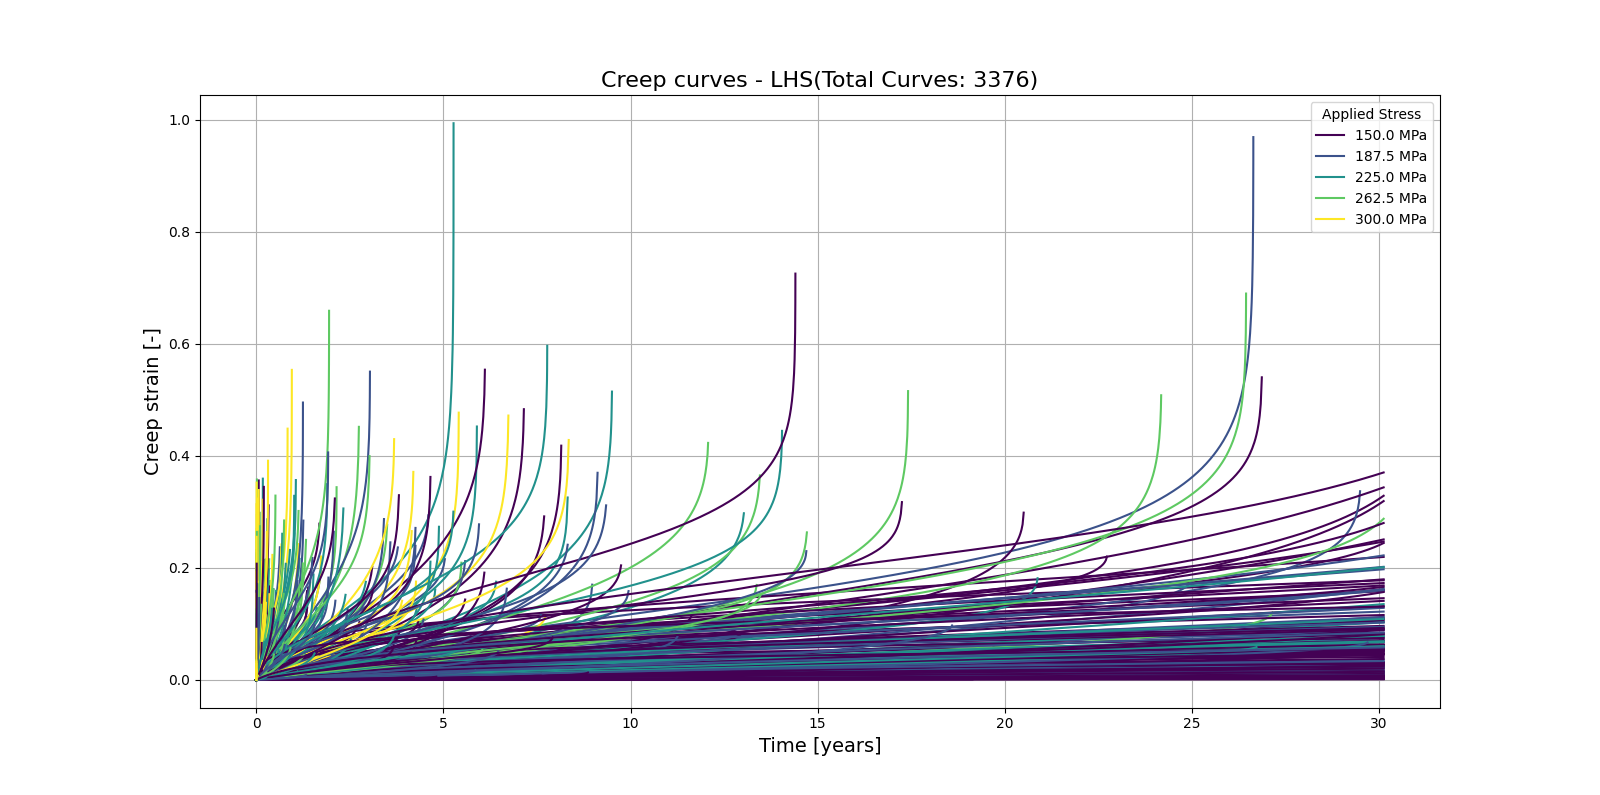
\includegraphics[width=1\textwidth]{figures/creep_curves_LHS.png}
		\caption{Ccreep strain-time curves from Lagamine simulations under different stress levels and material parameters.}
		\label{fig:fem_curves}
	\end{figure}

	\section{Creep Curve Representations}
	\label{Section::Results_CreepCurveRepresentations}
	
	\subsection{Empirical Models Curve Representations}
	\label{Subsection::Results_EmpiricalModels}
	
	This section presents the results of fitting the creep curves using the two empirical models described earlier: the $\theta$-projection model and the three-stage exponential creep model [\textit{see Section}~\ref{Subsection::Empirical_Models}].
	
	\subsubsection{1. $\theta$-Projection Model Fit}
	\label{Subsubsection::Results_ThetaProjection}
	
	Each creep curve was fitted using the $\theta$-projection model described in Equation~\ref{eq:theta_projection}.
	
	Figure~\ref{fig:theta_fit_whole_set} shows the original vs. fitted curve colour-coded by the deviation between them. The solid lines represent the fitted curves, while the dashed lines represent the original creep curves.
	
	\begin{figure}[H]
		\centering
		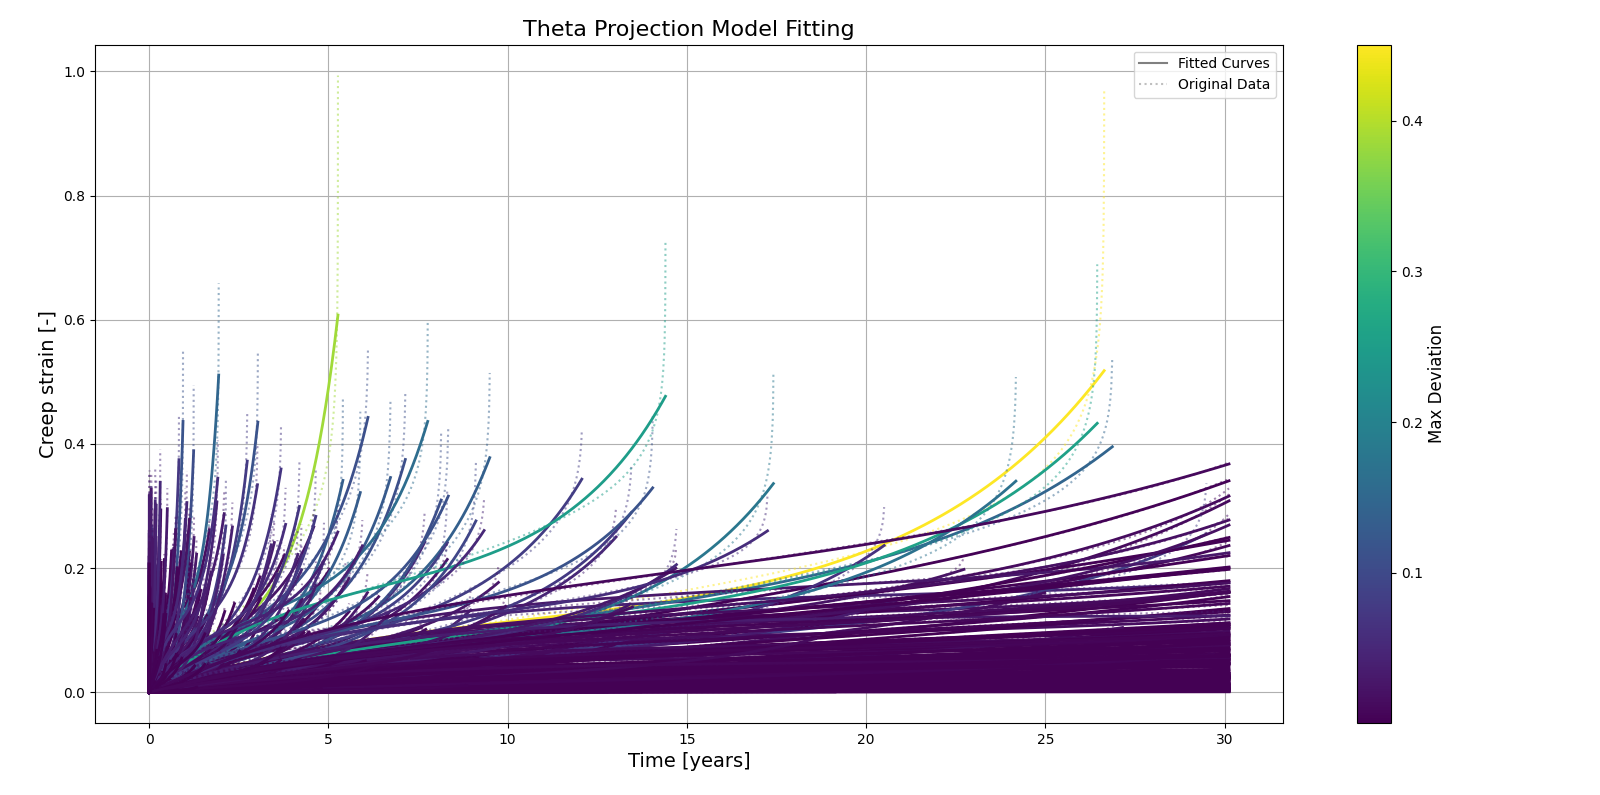
\includegraphics[width=0.95\textwidth]{figures/theta_projection_whole_dataset.png}
		\caption{$\theta$-projection fit by deviation.}
		\label{fig:theta_fit_whole_set}
	\end{figure}
	
	Figure~\ref{fig:theta_fit_max_deviation} shows the creep curve with the largest deviation from its fitted counterpart.
	
	\begin{figure}[H]
		\centering
		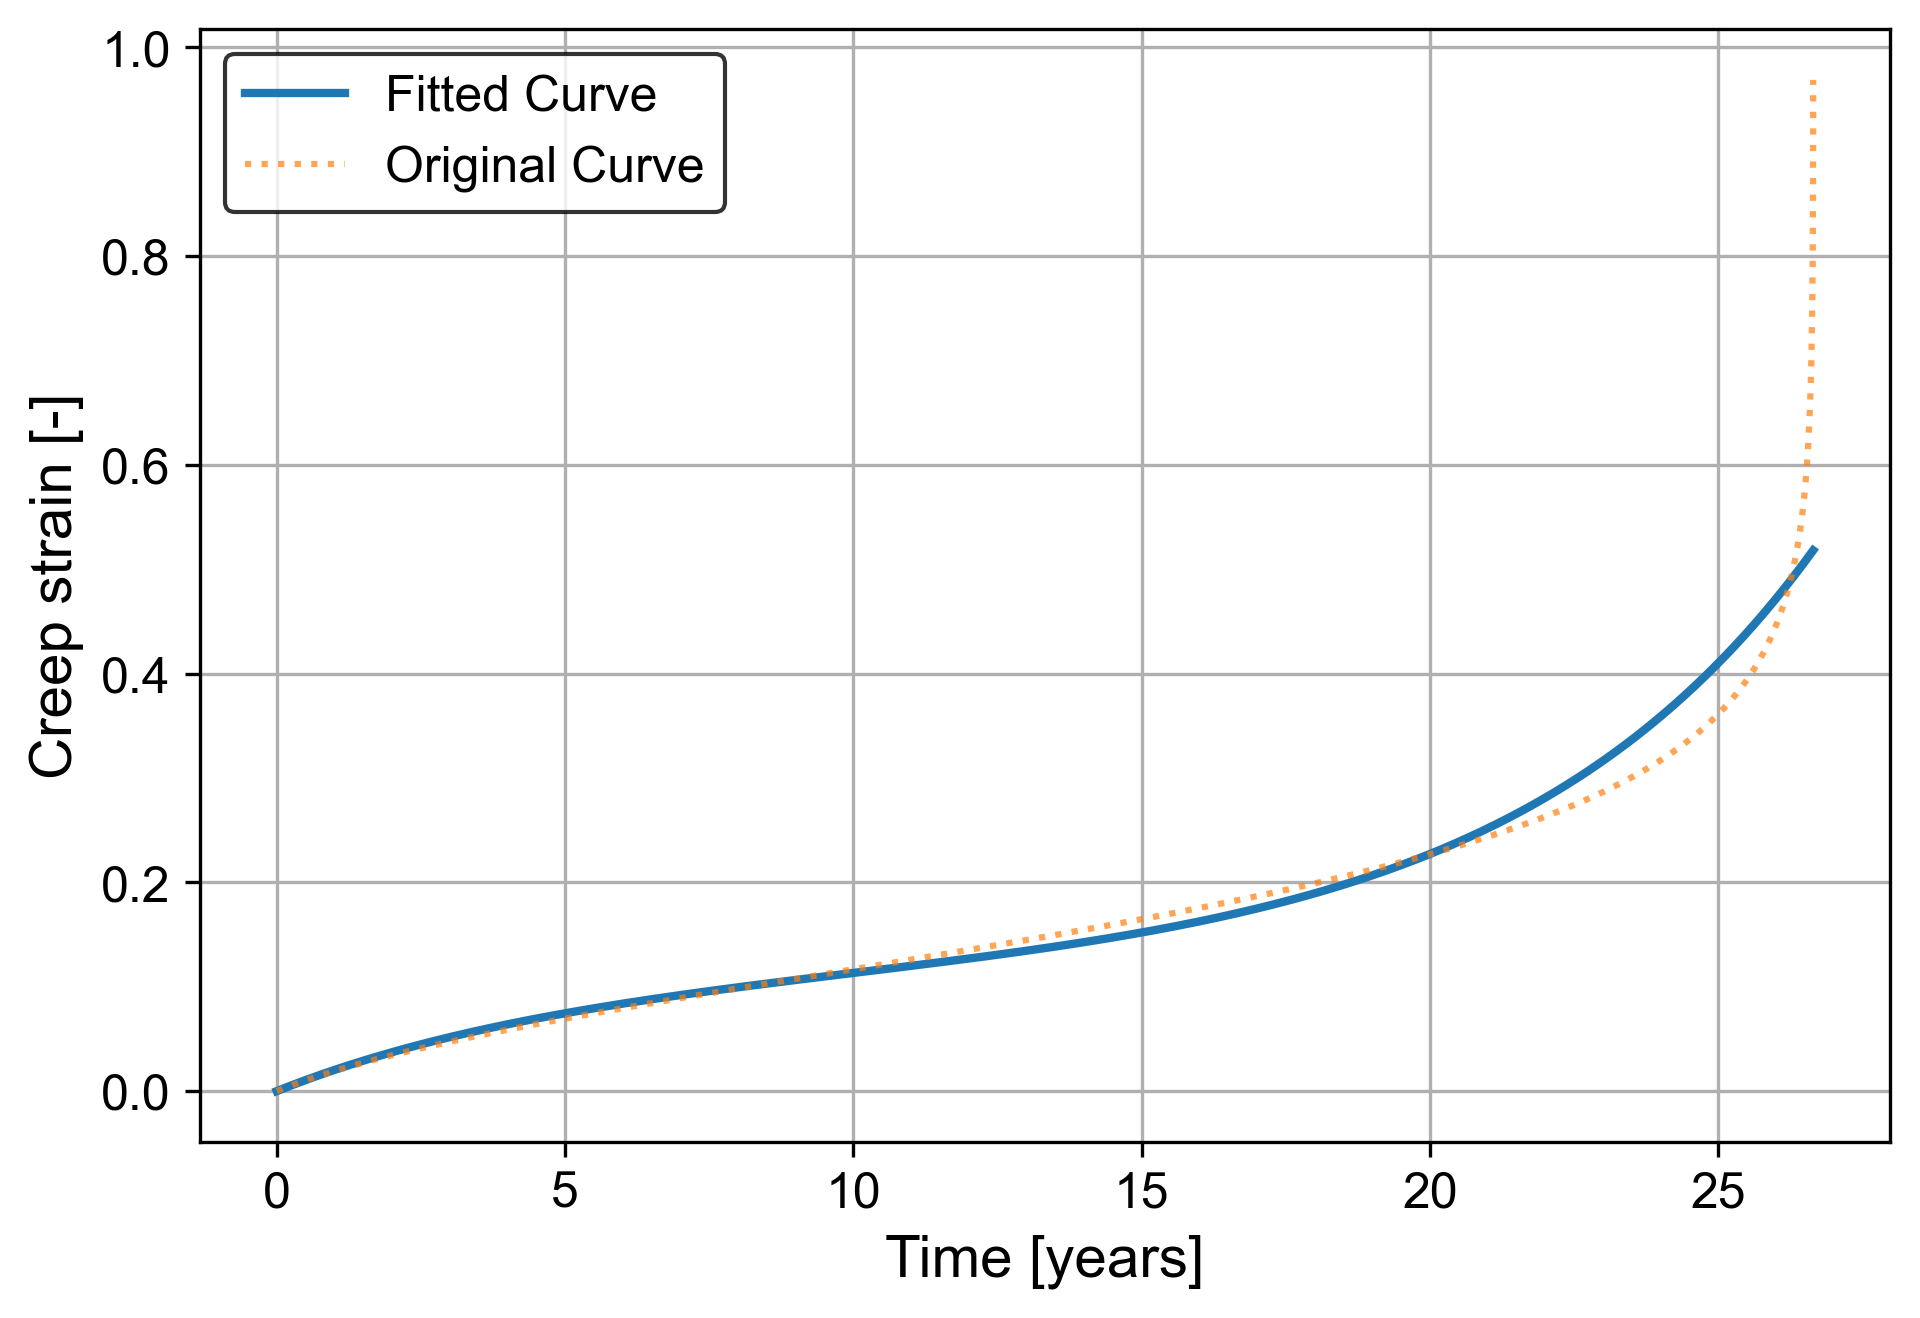
\includegraphics[width=0.85\textwidth]{figures/theta_projection_max_deviation.png}
		\caption{$\theta$-projection fit - Max deviation creep curve.}
		\label{fig:theta_fit_max_deviation}
	\end{figure}
		
	\subsubsection{2. Three Parameter Model Fit}
	\label{Subsubsection::Results_ThreeStage}
	
	The three-parameter exponential model (Equation~\ref{eq:three_stage_creep_equation}) was applied to the same dataset. It provided a continuous representation across all creep phases.
	

	Figure~\ref{fig:three_stage_fit_whole_dataset} shows the original vs. fitted curve colour coded by the deviation. Solid lines represent the fitted curves while the broken lines represent the original creep curves.
	
	\begin{figure}[H]
		\centering
		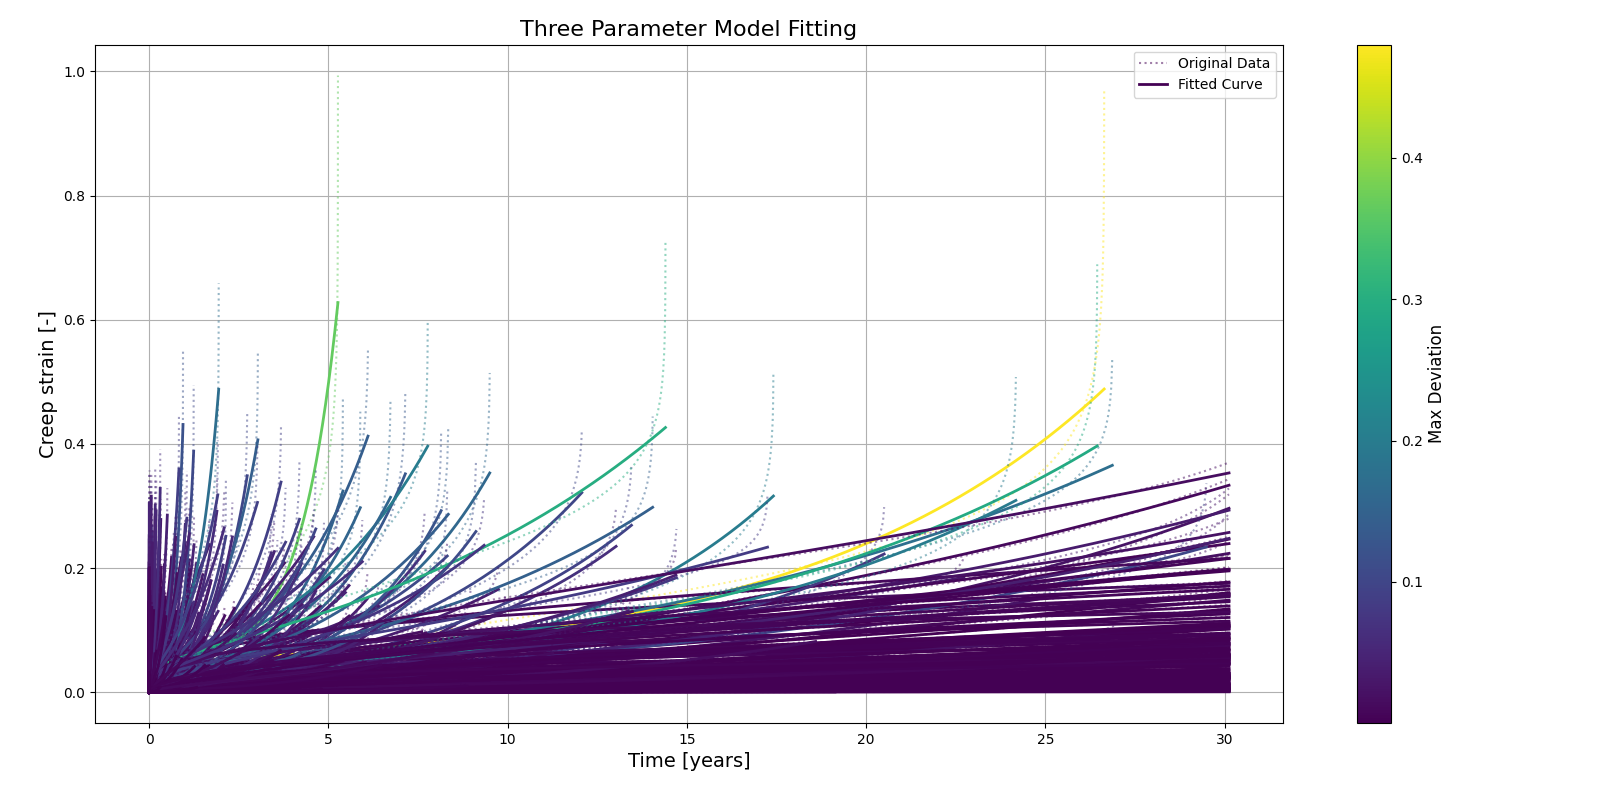
\includegraphics[width=0.95\textwidth]{figures/three_param_model_whole_dataset.png}
		\caption{Three Parameter creep model fit by deviation.}
		\label{fig:three_stage_fit_whole_dataset}
	\end{figure}
	
	Figure~\ref{fig:three_stage_fit_max_deviation} shows the creep curve with the poorest fit from the original.
	
	\begin{figure}[H]
		\centering
		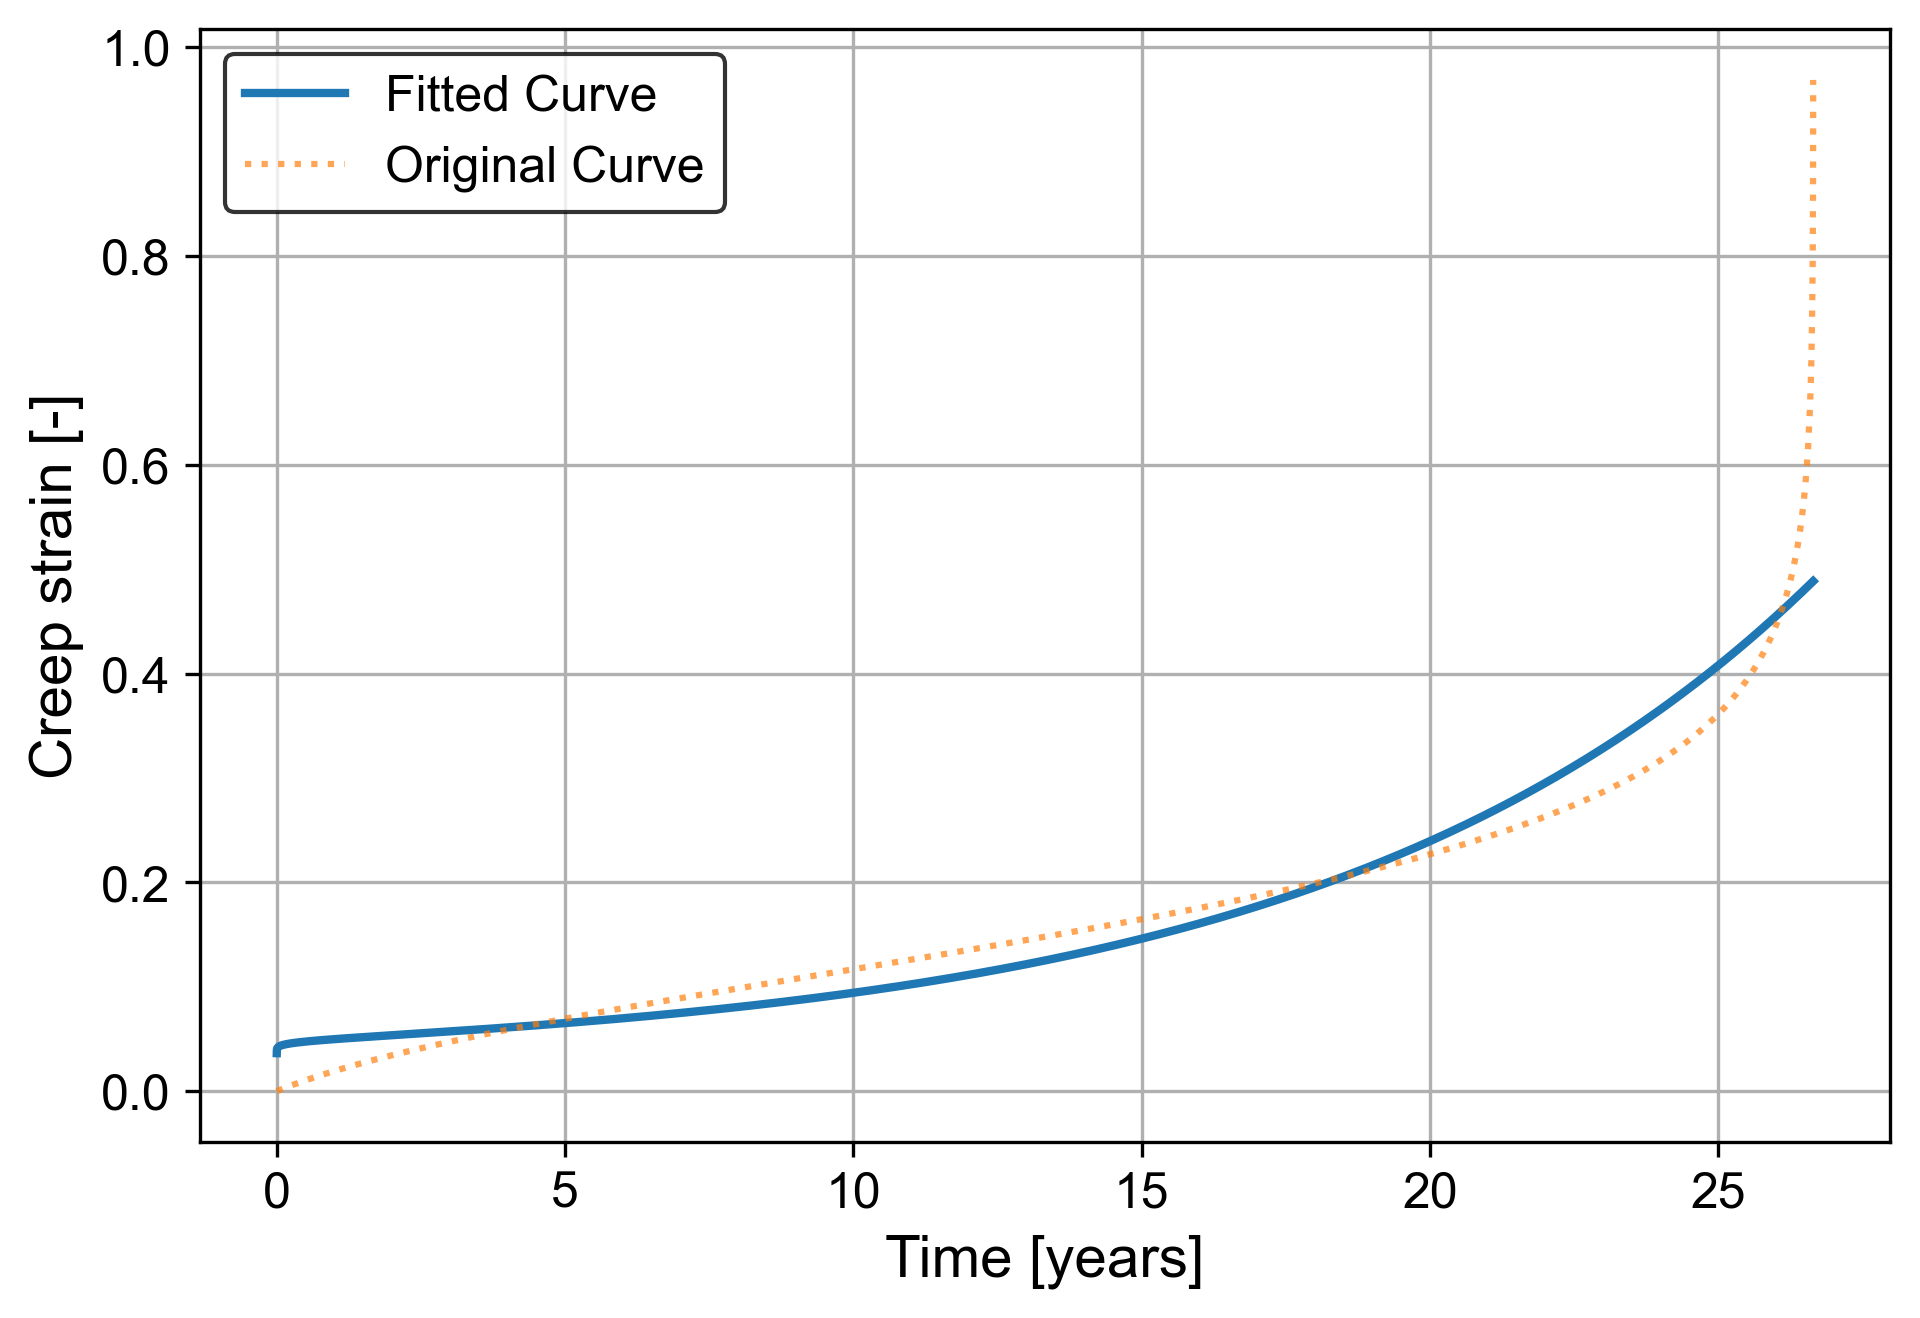
\includegraphics[width=0.85\textwidth]{figures/three_param_model_max_deviation.png}
		\caption{$\theta$-projection fit - Max deviation creep curve.}
		\label{fig:three_stage_fit_max_deviation}
	\end{figure}
	
	\subsection{Data-Driven Models}
	\label{Subsection::Results_DataDrivenModels}
	
	\subsubsection{1. Principal Component Analysis (PCA)}
	
	PCA was applied to the preprocessed creep strain-time data. The three strategies to handle the different input vector lengths had different results. For visualization, 6 random curves from the test set are plotted with the original creep curve against the reconstructed creep curve. This is done for all the three strategies. 
	
	\subsubsubsection{Zero Padding:}
	
	The variance captured by each principal component is summarized in Figure~\ref{fig:pca_variance_zero}.
	
	\begin{figure}[H]
		\centering
		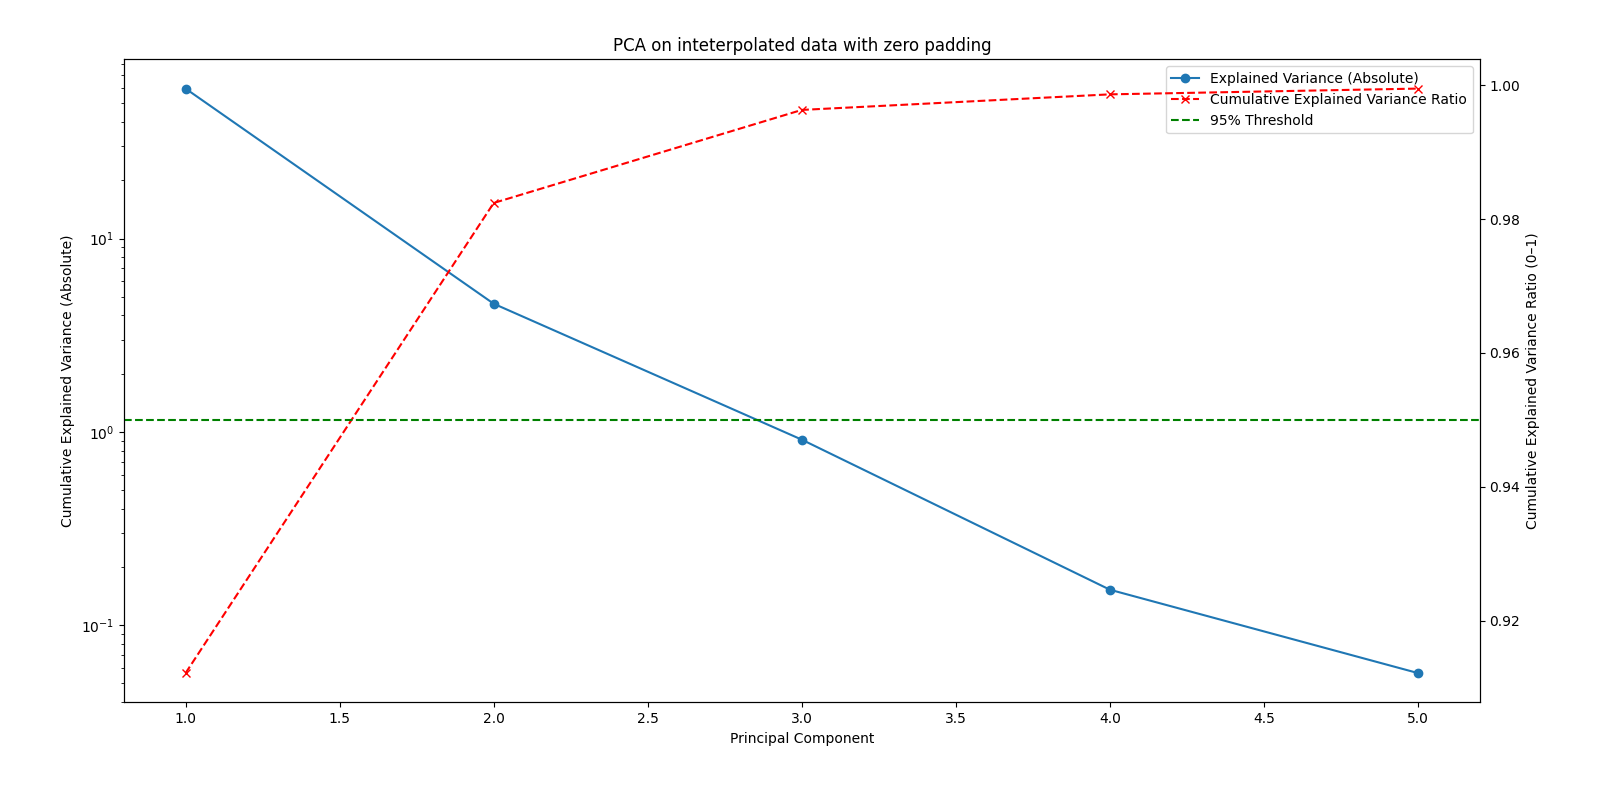
\includegraphics[width=0.65\textwidth]{figures/pca_var_zero_fill.png}
		\caption{Explained variance by each principal component (PCA).}
		\label{fig:pca_variance_zero}
	\end{figure}
	
	The first 2 components captured over 95\% of the total variance.	
	
	The original vs. the reconstructed creep curves with zero padding is shown in figure~\ref{fig:pca_zero_fill}.
	
	\begin{figure}[H]
		\centering
		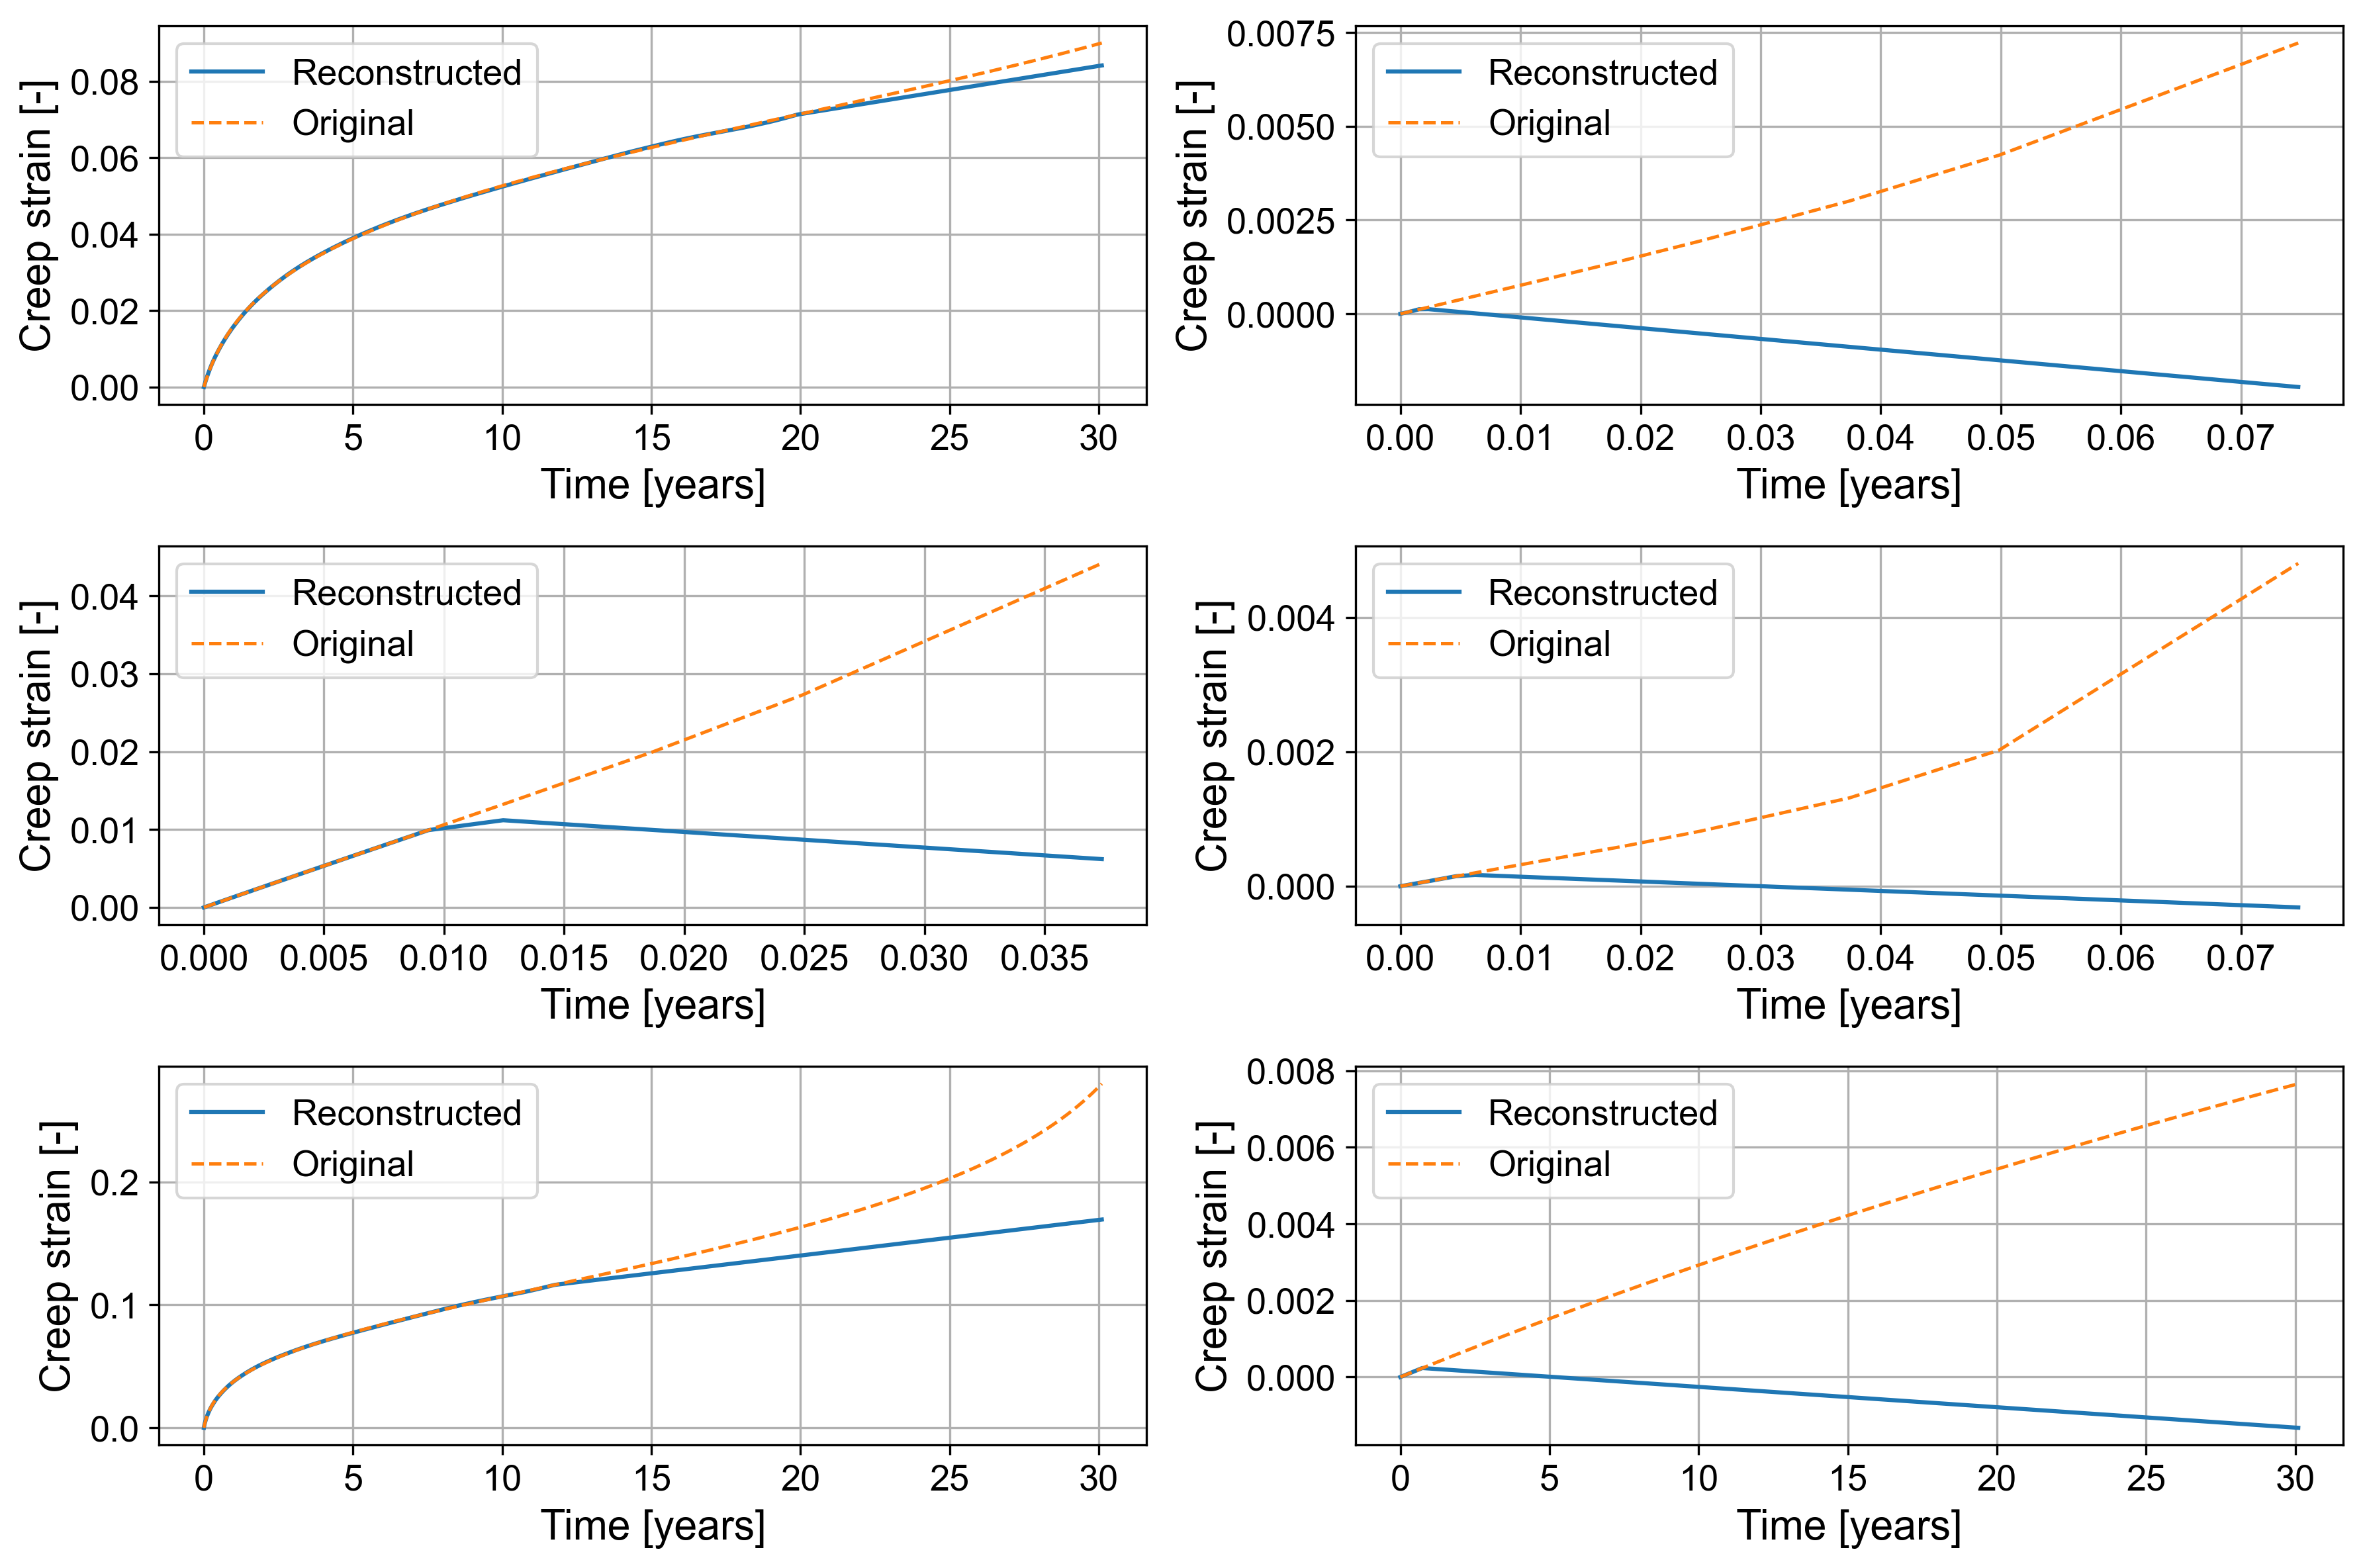
\includegraphics[width=1\textwidth]{figures/pca_reconstructed_curves_zero_fill.png}
		\caption{Original vs. Reconstructed Creep Curves(PCA) - Zero paddding.}
		\label{fig:pca_zero_fill}
	\end{figure}
	
	\subsubsubsection{Max Creep Strain Padding:}
	
	The variance captured by each principal component is summarized in Figure~\ref{fig:pca_variance_max}.
	
	\begin{figure}[H]
		\centering
		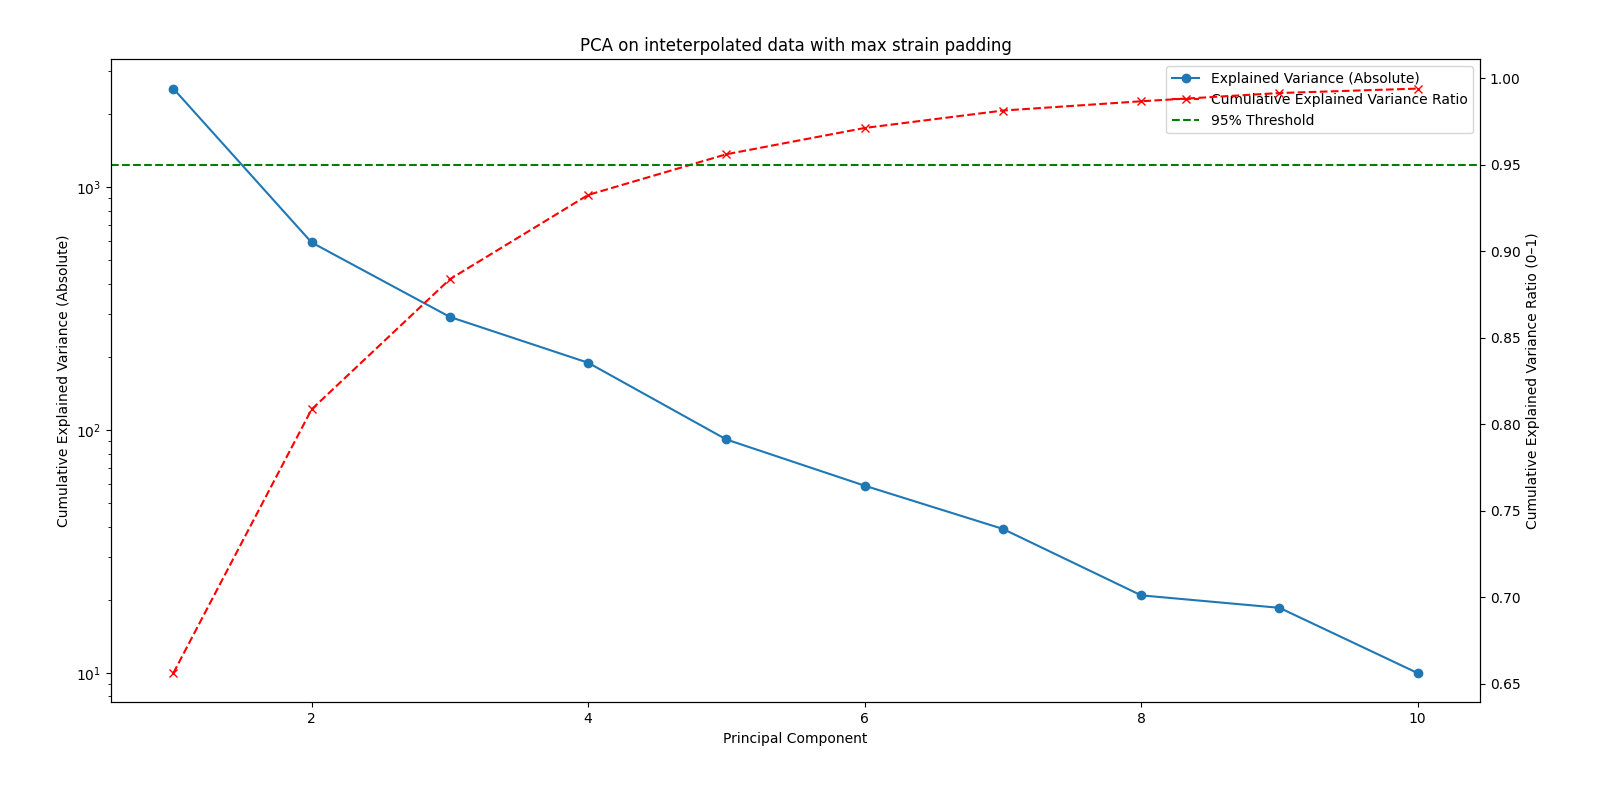
\includegraphics[width=0.65\textwidth]{figures/pca_var_max_fill.png}
		\caption{Explained variance by each principal component (PCA).}
		\label{fig:pca_variance_max}
	\end{figure}
	
	The first 5 components captured over 95\% of the total variance.	
	
	The original vs. the reconstructed creep curves with the maximum creep strain padding is shown in figure~\ref{fig:pca_max_fill}.
	
	\begin{figure}[H]
		\centering
		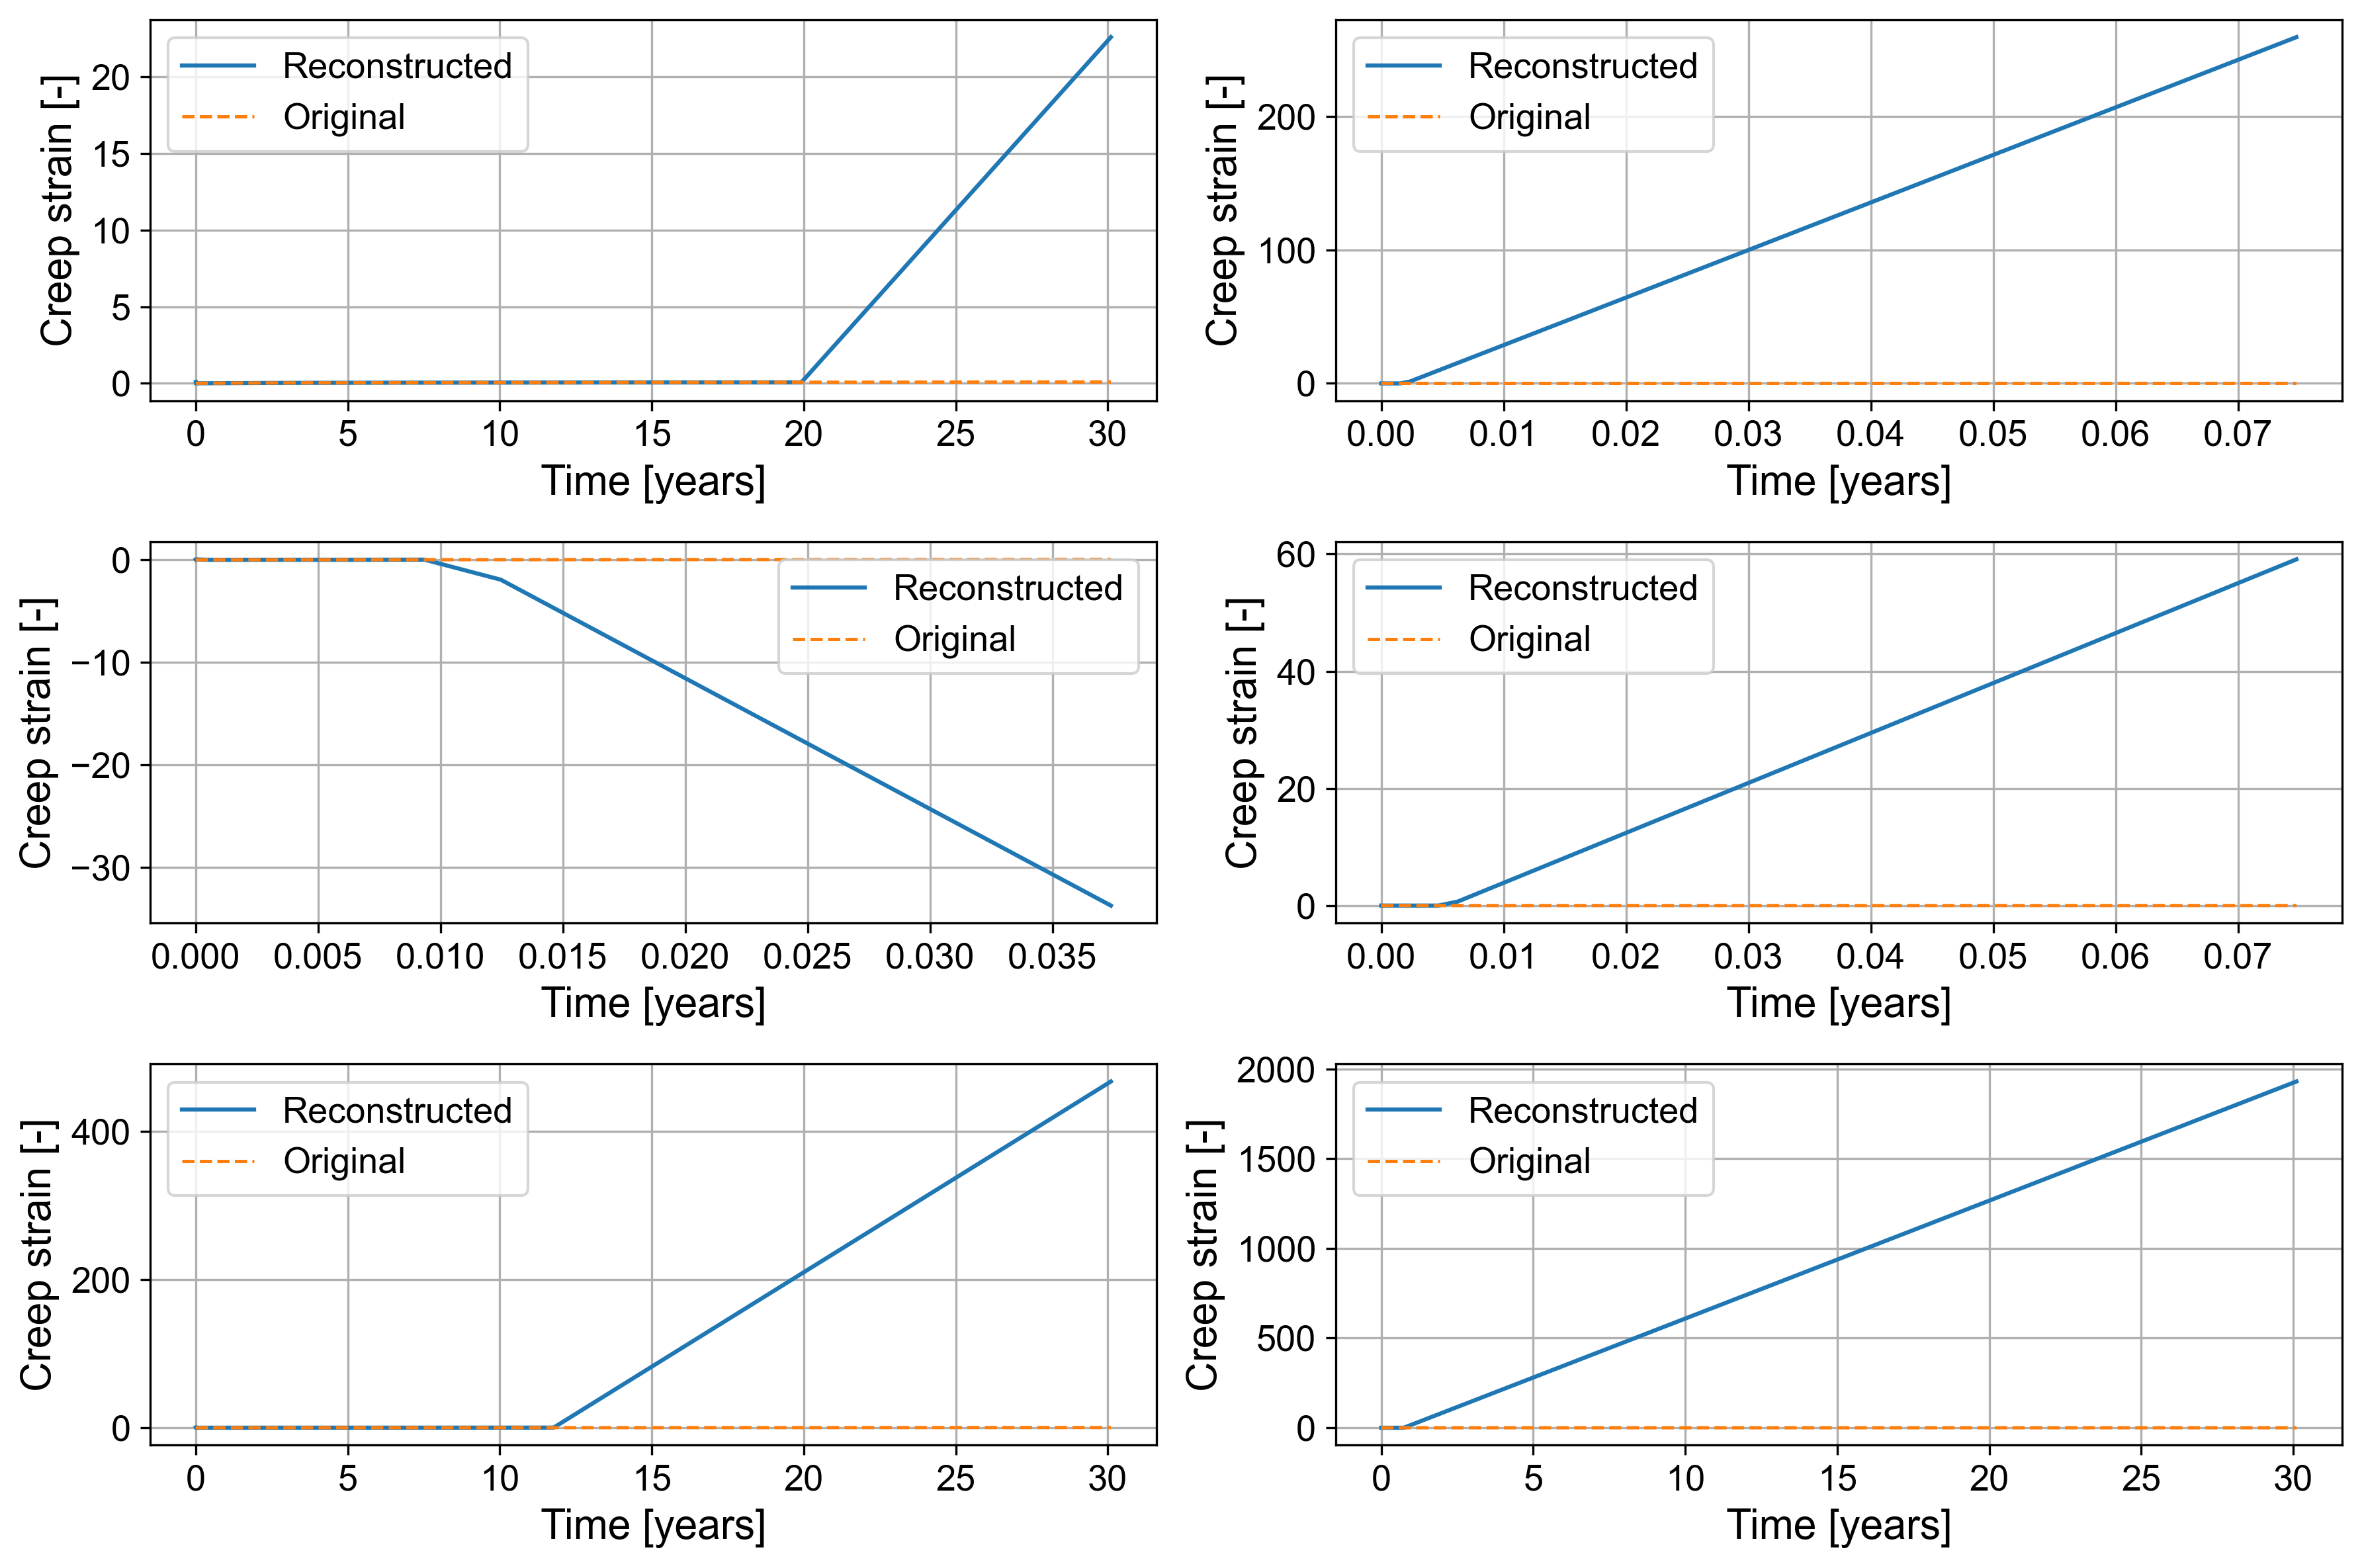
\includegraphics[width=1\textwidth]{figures/pca_reconstructed_curves_max_fill.png}
		\caption{Original vs. Reconstructed Creep Curves(PCA) - Max creep strain paddding.}
		\label{fig:pca_max_fill}
	\end{figure}
	
	\subsubsubsection{Normalization by Rupture time:}
	
	The variance captured by each principal component is summarized in Figure~\ref{fig:pca_variance_norm}.
	
	\begin{figure}[H]
		\centering
		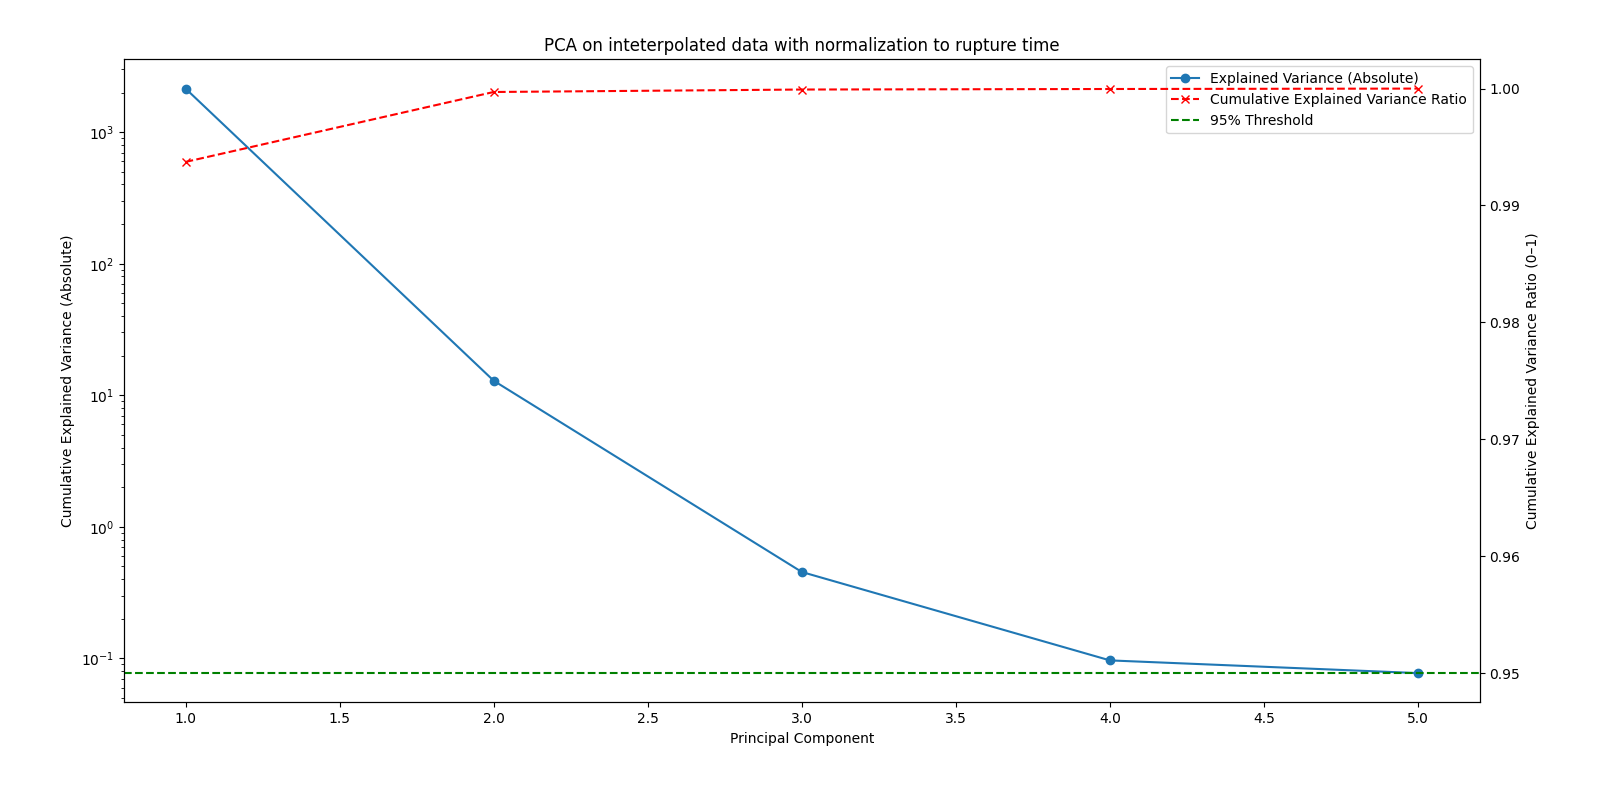
\includegraphics[width=0.65\textwidth]{figures/pca_var_norm.png}
		\caption{Explained variance by each principal component (PCA).}
		\label{fig:pca_variance_norm}
	\end{figure}
	
	The first component captured over 95\% of the total variance.	
	
	The original vs. the reconstructed creep curves with the normalization by rupture time approach is shown in figure~\ref{fig:pca_norm_rupture_time}.
	
	\begin{figure}[H]
		\centering
		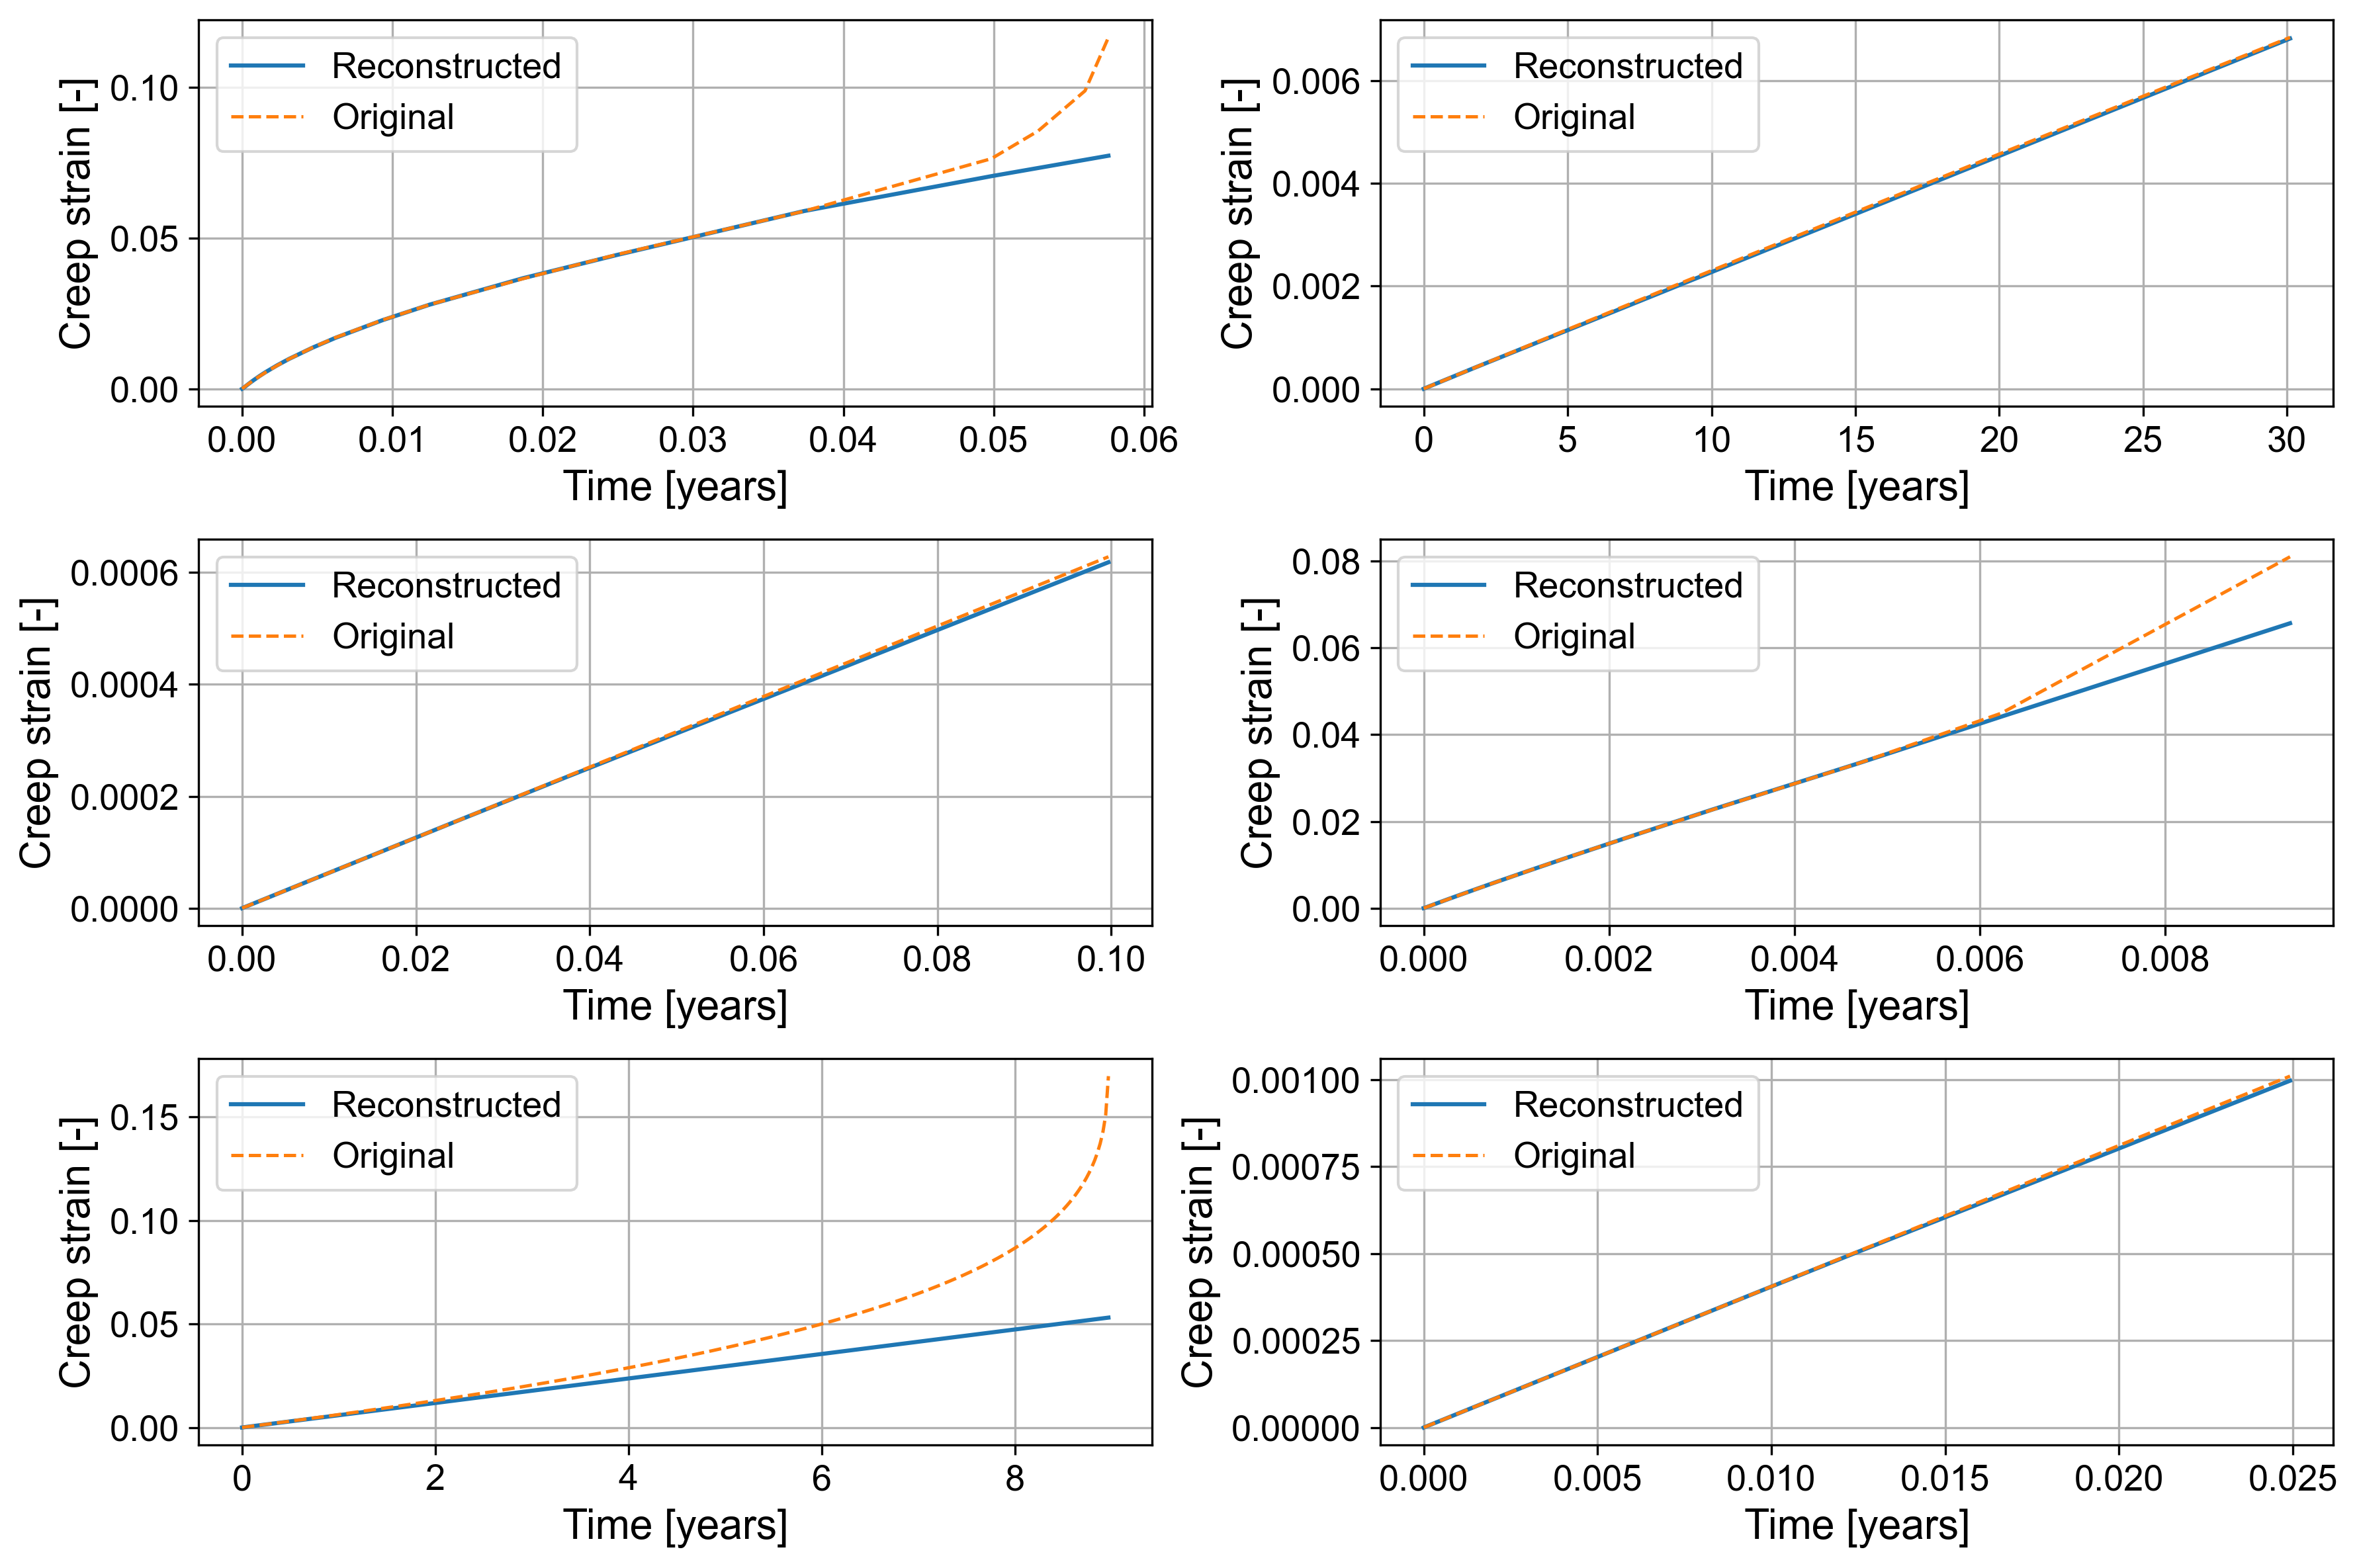
\includegraphics[width=1\textwidth]{figures/pca_reconstructed_curves_norm.png}
		\caption{Original vs. Reconstructed Creep Curves(PCA) - Normalization by rupture time approach.}
		\label{fig:pca_norm_rupture_time}
	\end{figure}
	
	\subsubsection{2. Kernel PCA (KPCA)}
	
	Kernel PCA using polynomial and RBF kernels to the preprocessed creep strain-time data. Similar to PCA, KPCA shows different results for the different data preprocessing approaches. 
	
	\subsubsubsection{Zero Padding:}
	
	\begin{table}[ht]
		\centering
		\caption{Best parameters for RBF and Polynomial kernels - Zero padding}
		\begin{tabular}{|l|l|l|}
			\hline
			\textbf{Kernel} & \textbf{Best Parameters} \\
			\hline
			RBF & $\{n\_components = 20,\ \gamma = 0.1\}$ \\
			Poly & $\{n\_components = 50,\ \text{degree} = 2,\ \gamma = 0.01,\ \text{coef}_0 = 1\}$  \\
			\hline
		\end{tabular}
		\label{tab:best_params_zero_fill}
	\end{table}
	
	The original vs. the reconstructed creep curves with zero padding is shown in figure~\ref{fig:kpca_zero_fill}.
	
	\begin{figure}[H]
		\centering
		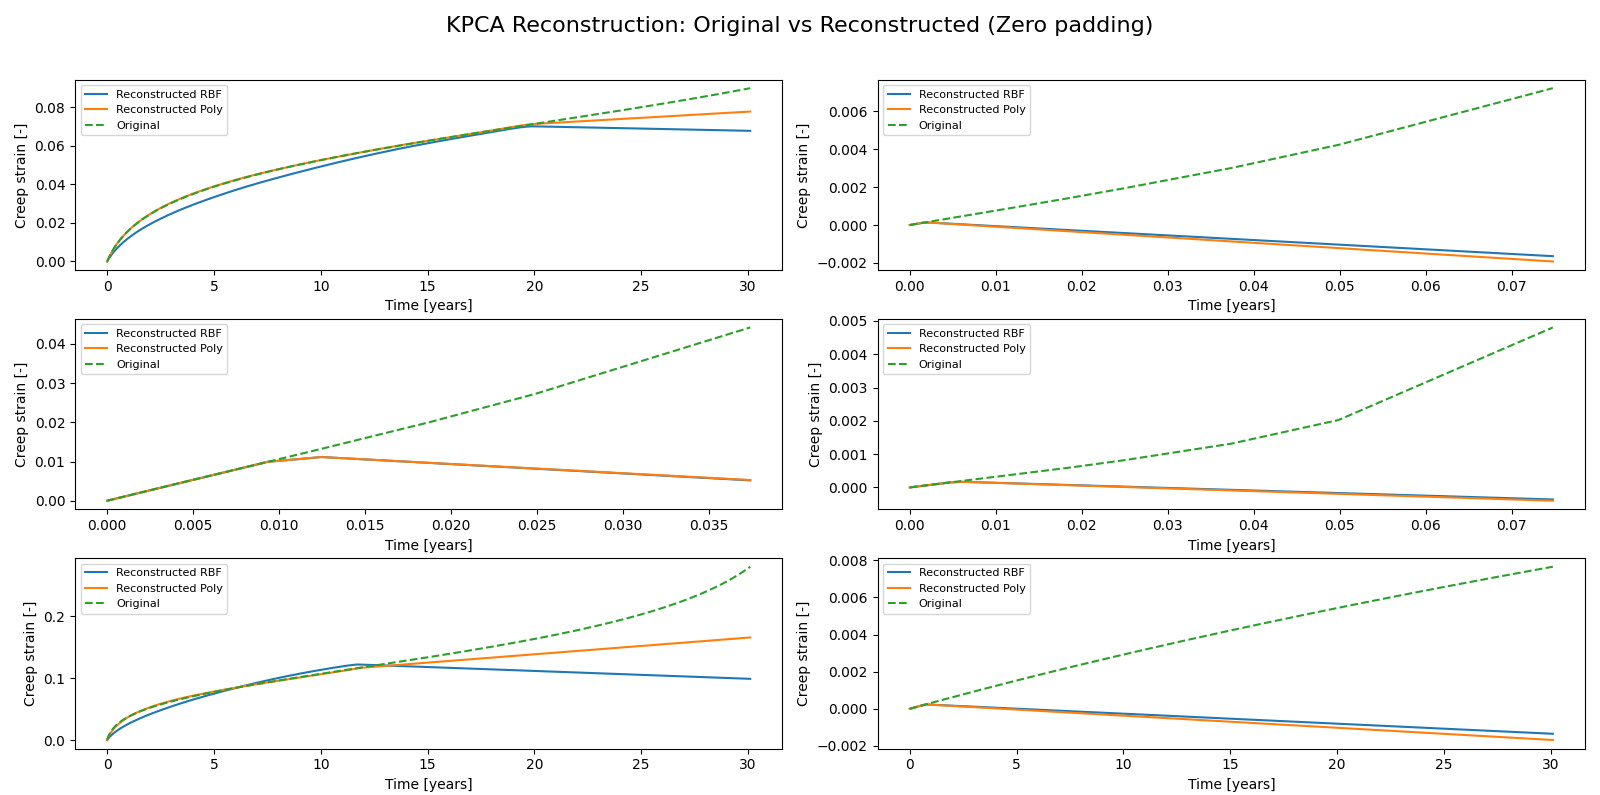
\includegraphics[width=1\textwidth]{figures/kpca_reconstructed_curves_zero_fill.png}
		\caption{Original vs. Reconstructed Creep Curves(KPCA) - Zero paddding.}
		\label{fig:kpca_zero_fill}
	\end{figure}
	
	\subsubsubsection{Max Creep Strain Padding:}
	
	\begin{table}[ht]
		\centering
		\caption{Best parameters for RBF and Polynomial kernels - Max strain padding}
		\begin{tabular}{|l|l|l|}
			\hline
			\textbf{Kernel} & \textbf{Best Parameters} \\
			\hline
			RBF & $\{n\_components = 50,\ \gamma = 0.01\}$ \\
			Poly & $\{n\_components = 50,\ \text{degree} = 3,\ \gamma = 0.001,\ \text{coef}_0 = 1\}$  \\
			\hline
		\end{tabular}
		\label{tab:best_params_max_fill}
	\end{table}
	
	The original vs. the reconstructed creep curves with the maximum creep strain padding is shown in figure~\ref{fig:kpca_max_fill}.
	
	\begin{figure}[H]
		\centering
		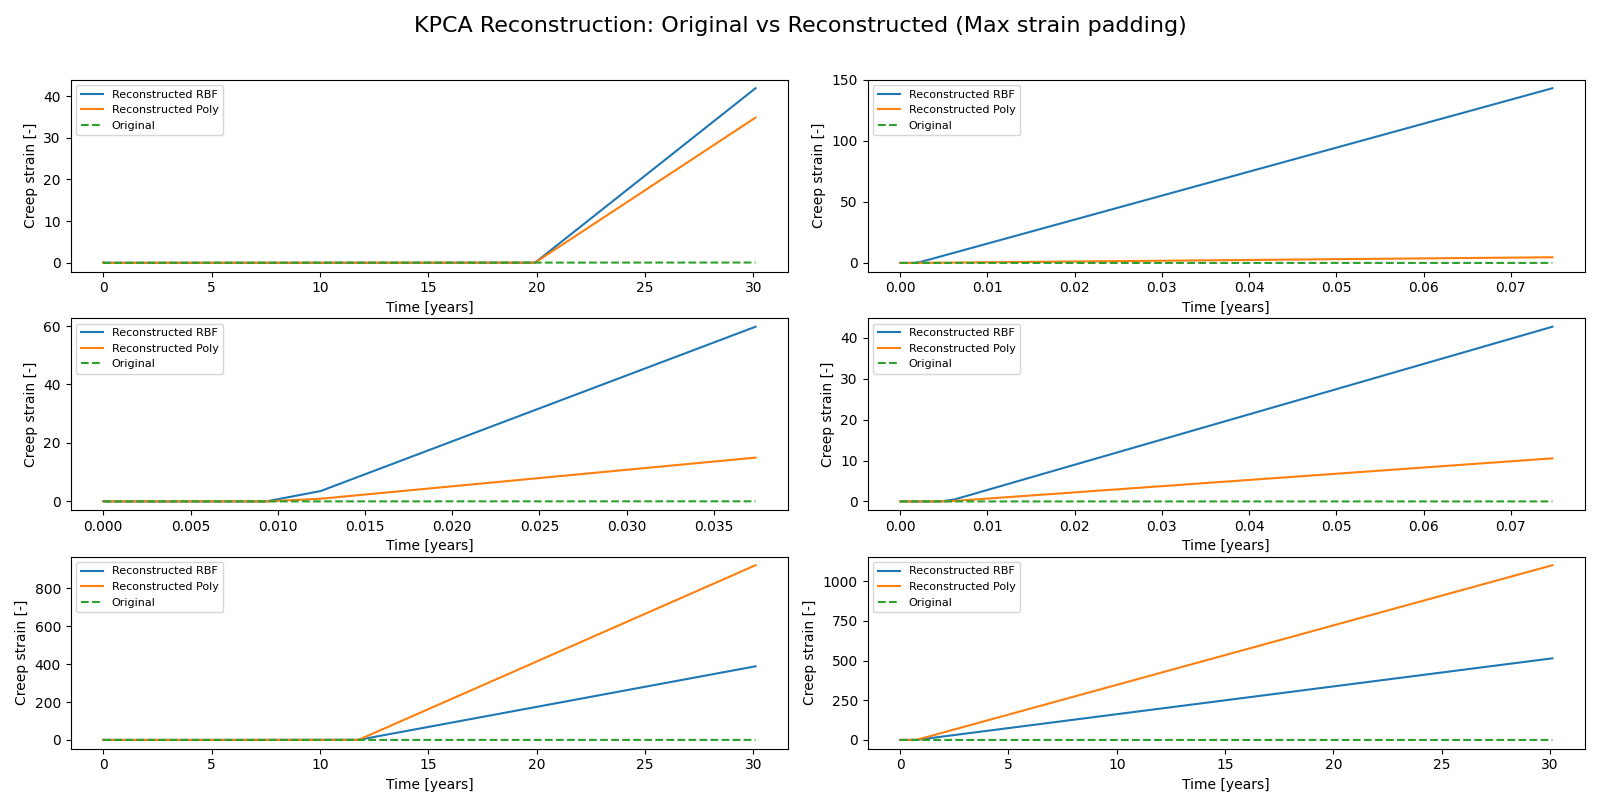
\includegraphics[width=1\textwidth]{figures/kpca_reconstructed_curves_max_fill.png}
		\caption{Original vs. Reconstructed Creep Curves(KPCA) - Max creep strain paddding.}
		\label{fig:kpca_max_fill}
	\end{figure}
	
	\subsubsubsection{Normalization by Rupture time:}
	
	\begin{table}[ht]
		\centering
		\caption{Best parameters for RBF and Polynomial kernels - Normalization by rupture time}
		\begin{tabular}{|l|l|l|}
			\hline
			\textbf{Kernel} & \textbf{Best Parameters} \\
			\hline
			RBF & $\{n\_components = 50,\ \gamma = 1\}$ \\
			Poly & $\{n\_components = 20,\ \text{degree} = 2,\ \gamma = 0.01,\ \text{coef}_0 = 1\}$  \\
			\hline
		\end{tabular}
		\label{tab:best_params_norm}
	\end{table}
	
	The original vs. the reconstructed creep curves with the normalization by rupture time approach is shown in figure~\ref{fig:kpca_norm_rupture_time}.
	
	\begin{figure}[H]
		\centering
		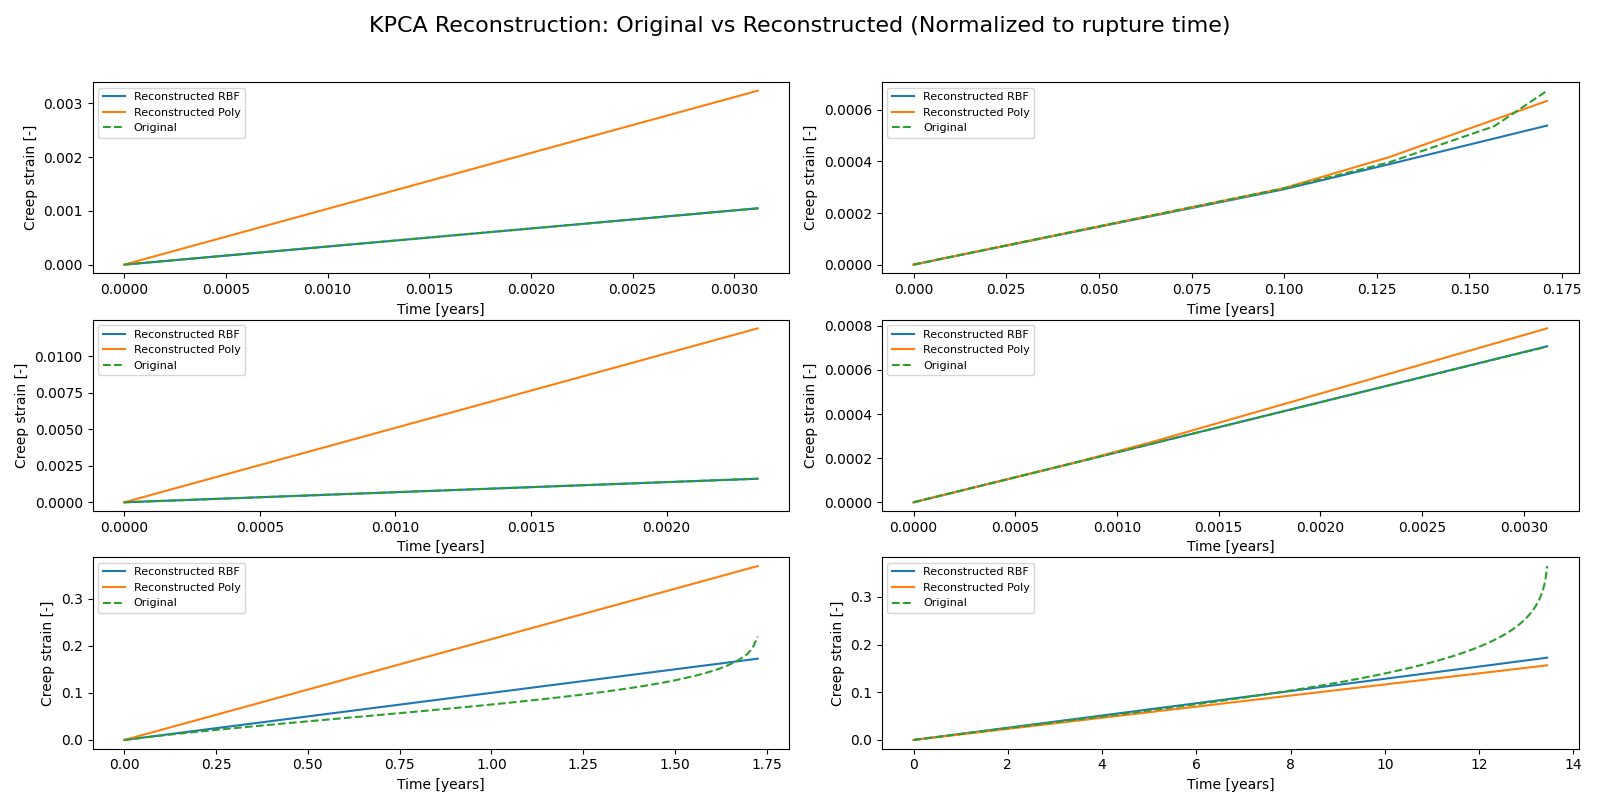
\includegraphics[width=1\textwidth]{figures/kpca_reconstructed_curves_norm.png}
		\caption{Original vs. Reconstructed Creep Curves(KPCA) - Normalization by rupture time approach.}
		\label{fig:kpca_norm_rupture_time}
	\end{figure}
	
	\subsection{Morch Model Parameter Representations (Inverse Model)}
	\label{Subsection::Results_Supervised}
	
	The parity plots for the seven Morch model parameters are shown in this section for each of the Regression models. The data points are coloured by the stress/load applied.
	
	\subsubsubsection{Random Forest Regression}
	
	Figure~\ref{fig:RF_regression} shows the parity plot for the Morch material model parameters as predicted by the Random Forest Regressor.
	
	\begin{figure}[H]
		\centering
		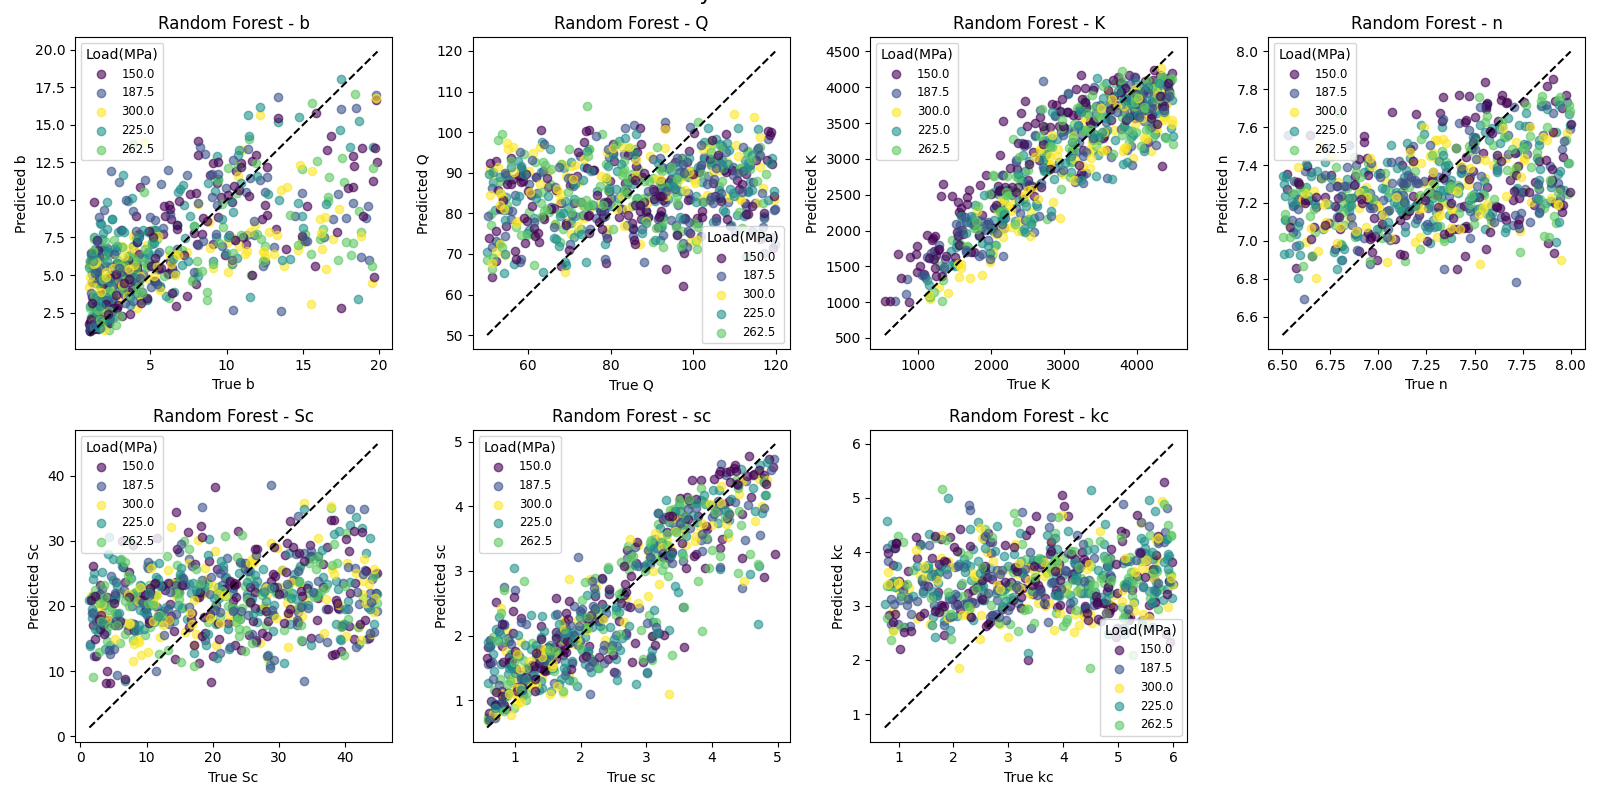
\includegraphics[width=0.95\textwidth]{figures/RF_parity_colored_by_load.png}
		\caption{Parity plot for the material model parameters predicted by random forest regressor.}
		\label{fig:RF_regression}
	\end{figure}
	
	\subsubsubsection{Gradient Boosting Regression}
	
	Figure~\ref{fig:GB_regression} shows the parity plot for the Morch material model parameters as predicted by the Gradient Boosting Regressor.
	
	\begin{figure}[H]
		\centering
		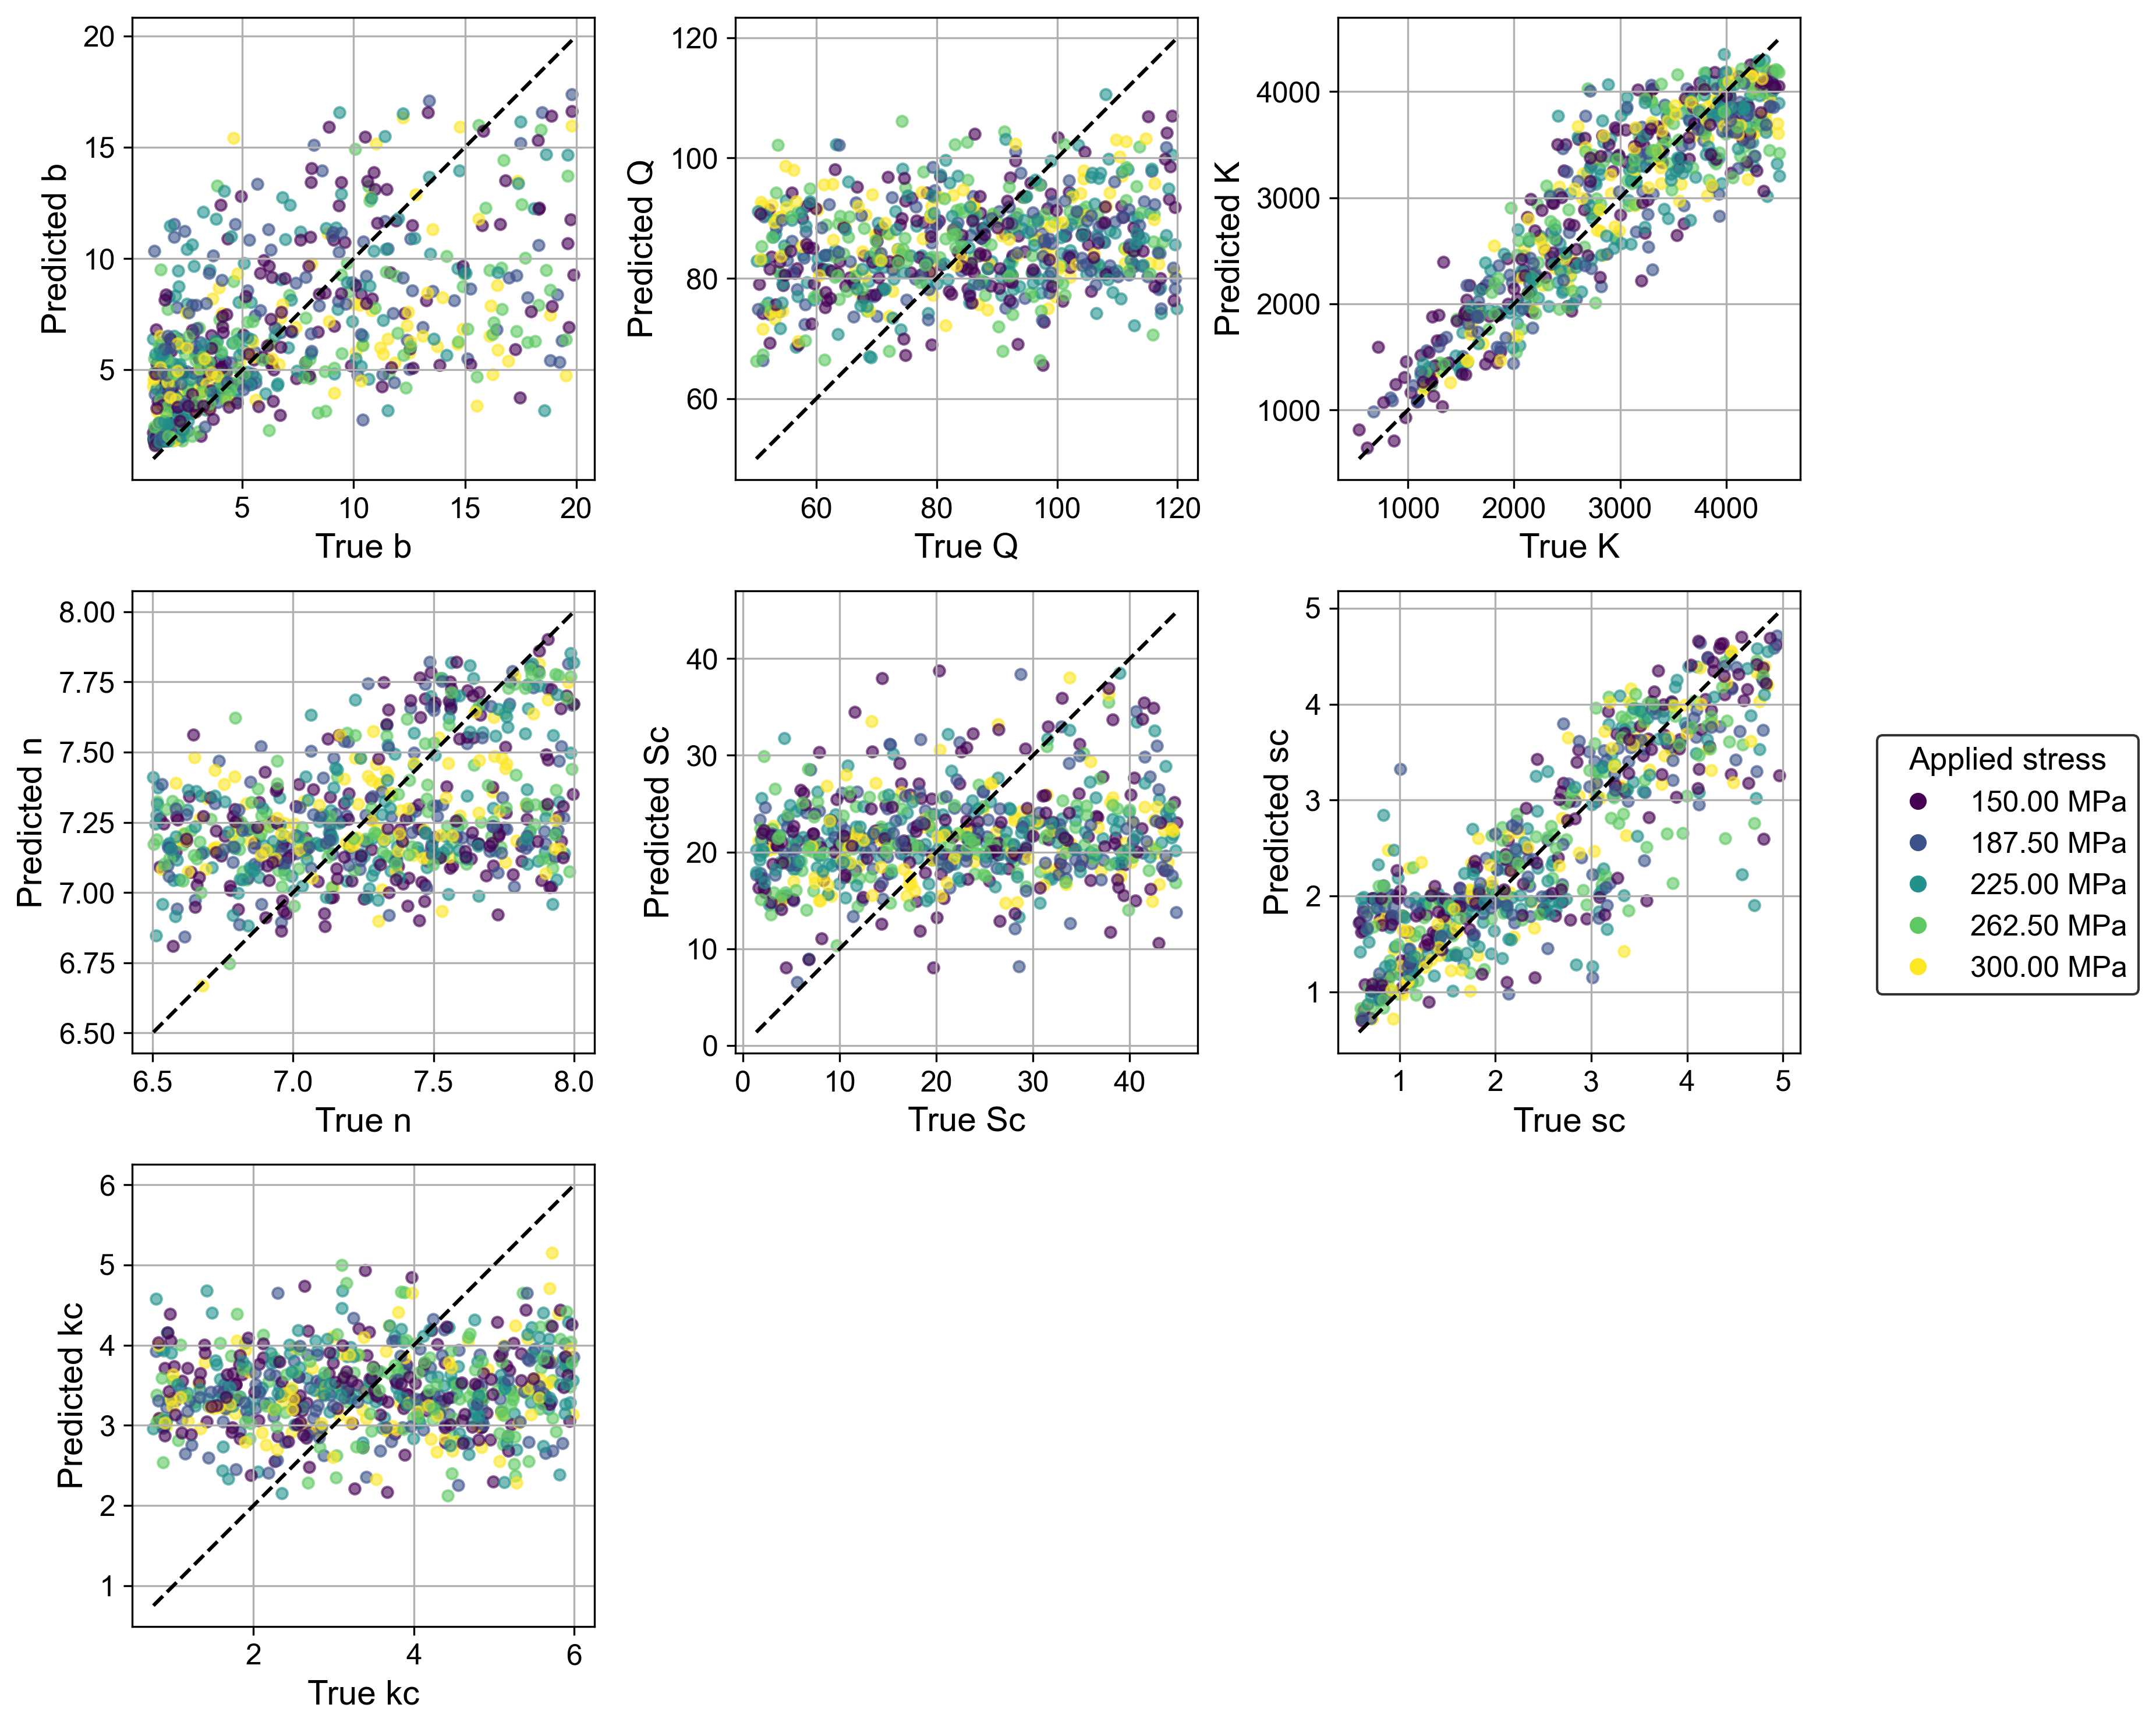
\includegraphics[width=0.95\textwidth]{figures/GB_parity_colored_by_load.png}
		\caption{Parity plot for the material model parameters predicted by gradient boosting regressor.}
		\label{fig:GB_regression}
	\end{figure}
	
	\subsubsubsection{Stacking Regression}
	
	Figure~\ref{fig:stacking_regression} shows the parity plot for the Morch material model parameters as predicted by the Stacking Regressor.
	
	\begin{figure}[H]
		\centering
		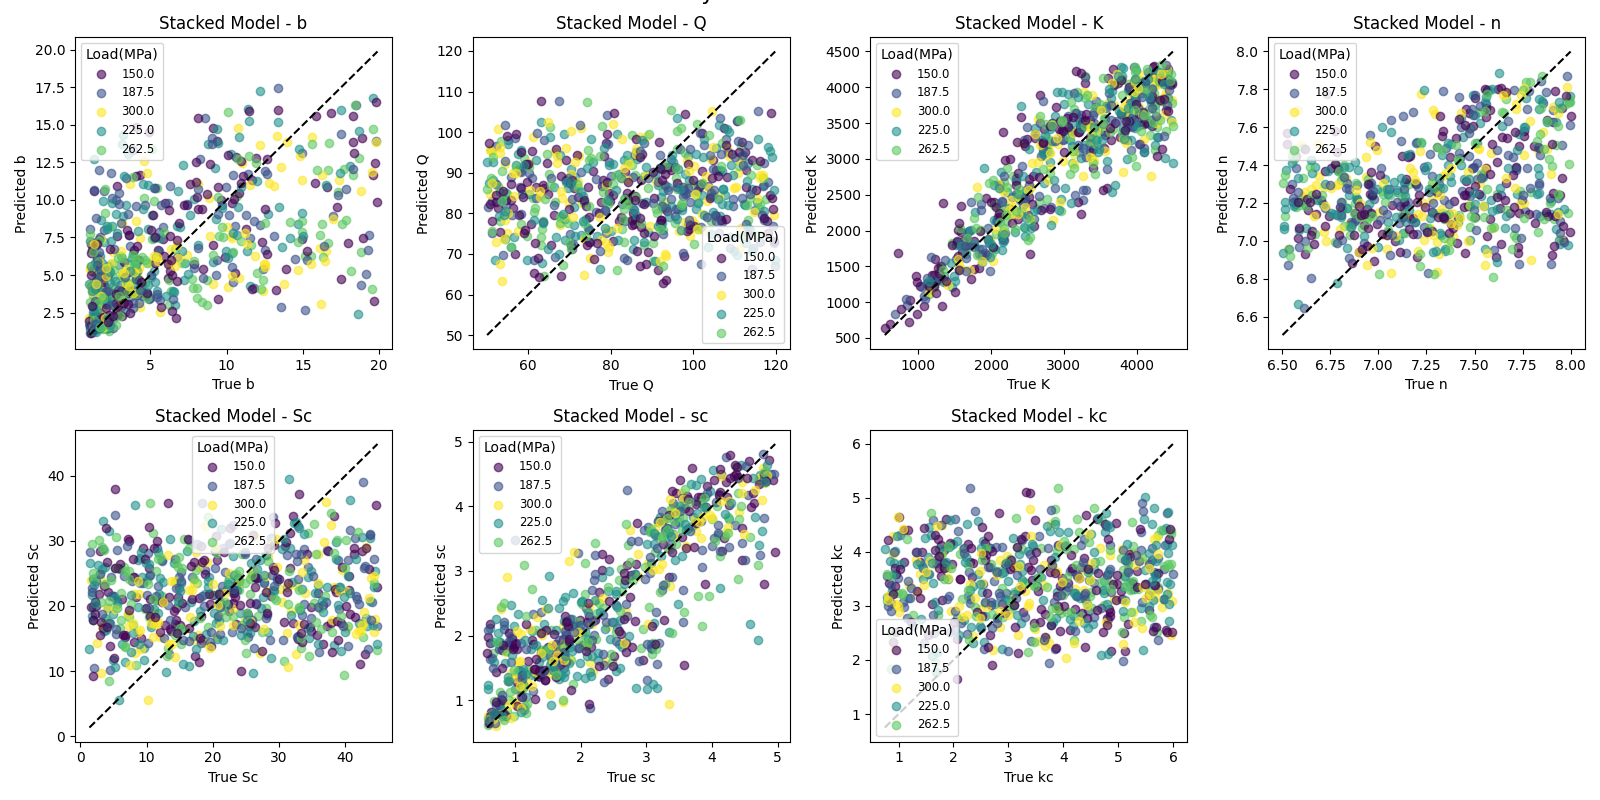
\includegraphics[width=0.95\textwidth]{figures/SM_parity_colored_by_load.png}
		\caption{Parity plot for the material model parameters predicted by stacking regressor.}
		\label{fig:stacking_regression}
	\end{figure}
	
	\subsubsubsection{Voting Regression}
	
	Figure~\ref{fig:voting_regression} shows the parity plot for the Morch material model parameters as predicted by the Voting Regressor.
	
	\begin{figure}[H]
		\centering
		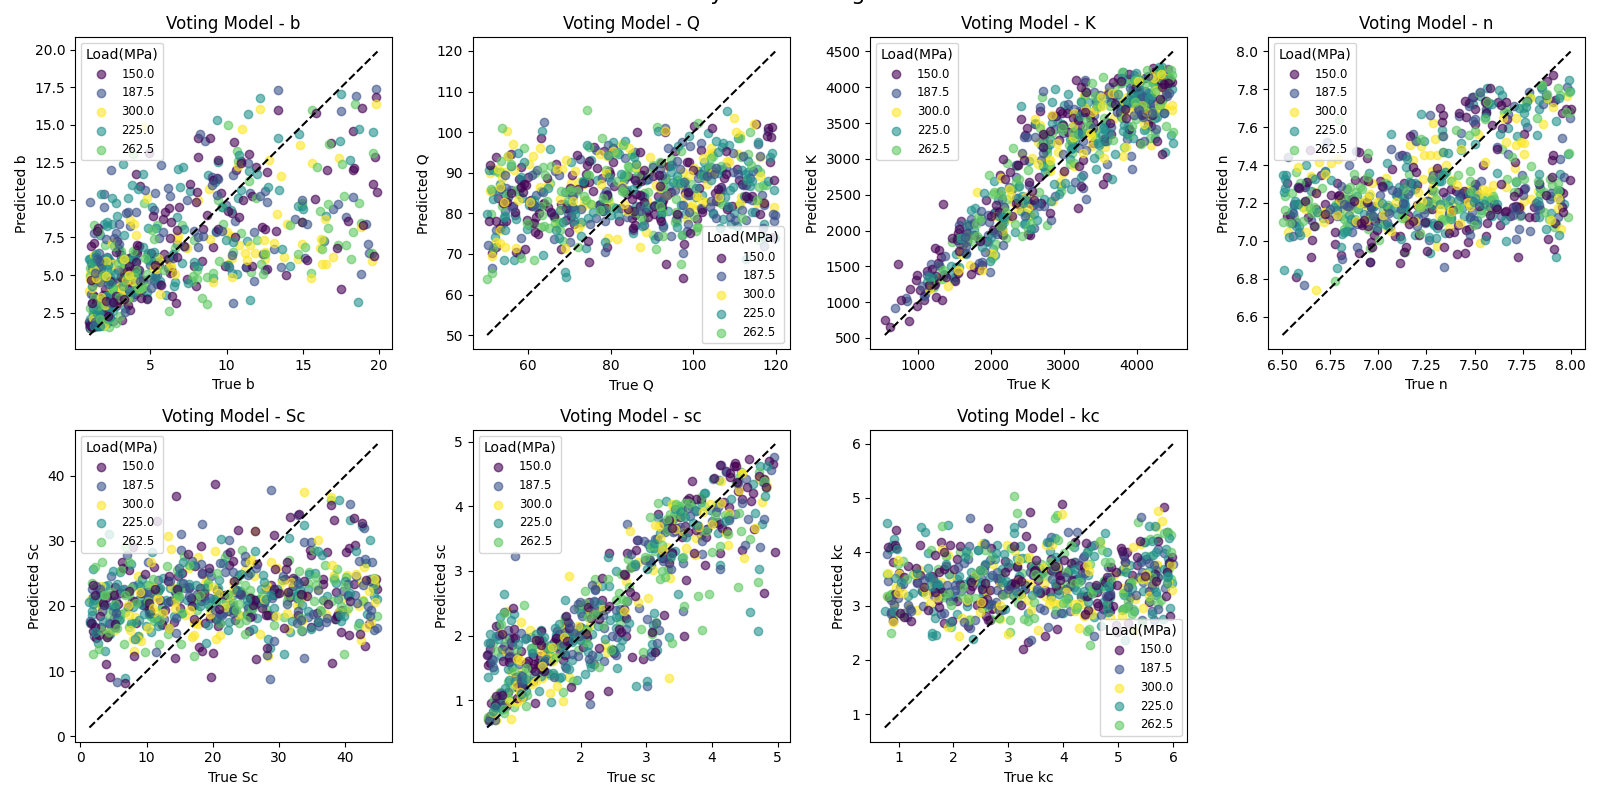
\includegraphics[width=0.95\textwidth]{figures/VM_parity_colored_by_load.png}
		\caption{Parity plot for the material model parameters predicted by voting regressor.}
		\label{fig:voting_regression}
	\end{figure}
	 
	Each model was evaluated on the 20\% test set using the metrics described in Section~\ref{Section::Evaluation}. Table~\ref{tab:model_performance} summarizes the mean absolute error (MAE) and $R^2$-score for predicting material model parameters.
	
	\begin{table}[ht]
		\centering
		\caption{Model performance comparison using MAE and $R^2$ score}
		\begin{tabular}{|l|c|c|}
			\hline
			\textbf{Model} & \textbf{Mean Absolute Error (MAE)} & \boldmath$R^2$ \\
			\hline
			Random Forest    & 58.3825 & 0.2890 \\
			Gradient Boosting & 53.9970 & 0.2830 \\
			Stacking Model   & 56.7212 & 0.1904 \\
			Voting Model     & 52.4986 & 0.2996 \\
			\hline
		\end{tabular}
		\label{tab:model_performance}
	\end{table}
	
	Since the Voting model shows better results among the four, it is used to generate creep curves from the finite element solver using the predicted material parameters. The figure~\ref{fig:curve_recon_model_params} shows the comparison of the original vs. the reconstructed creep curves.	
		
	\begin{figure}[H]
		\centering
		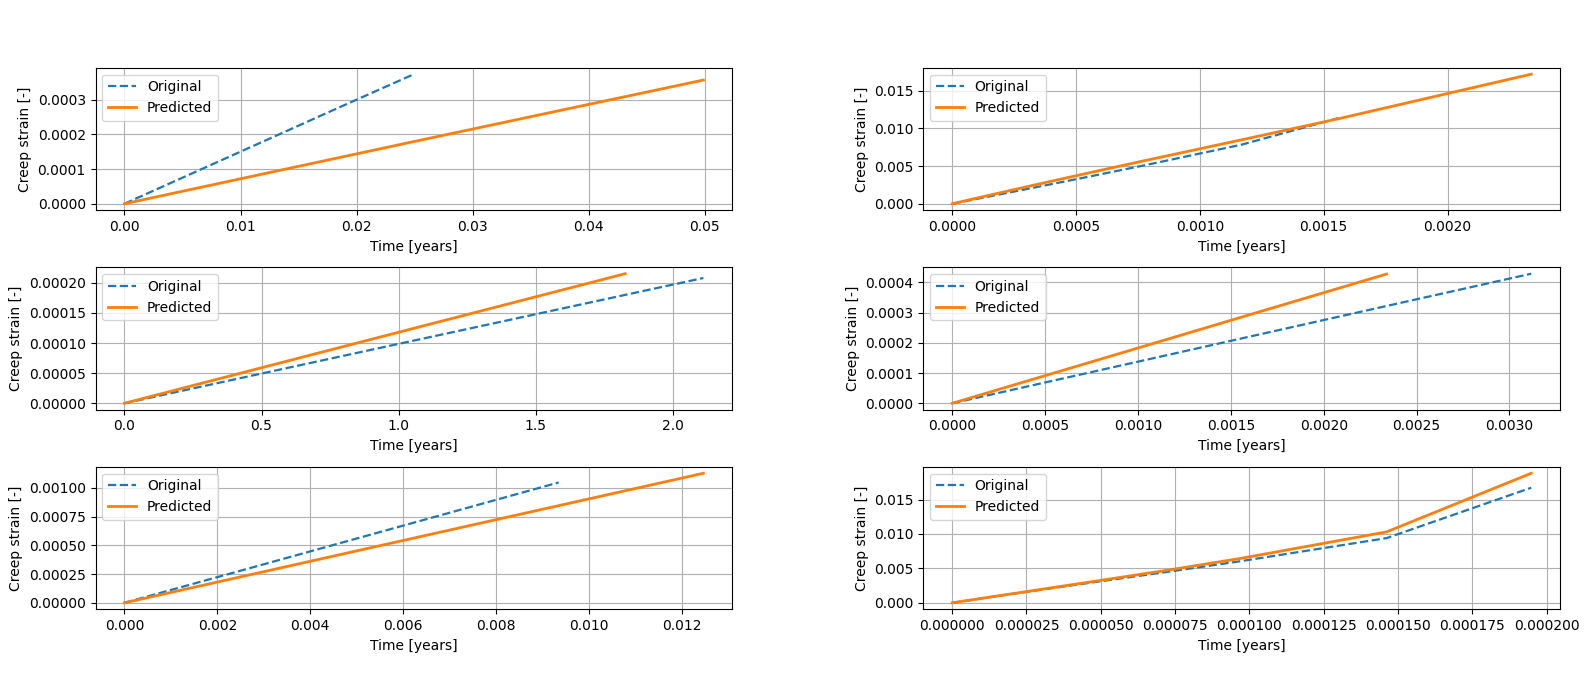
\includegraphics[width=1\textwidth]{figures/creep_comparison_from_model_params.png}
		\caption{Comparison of predicted and actual creep curves using Voting Regressor on test data.}
		\label{fig:curve_recon_model_params}
	\end{figure}
	
	\subsection{Model Comparison}
	\label{Subsection::Results_ModelComparison}
	
	The models discussed in section~\ref{Section::Results_CreepCurveRepresentations} are compared based on metrics like RMSE, minimum creep rate error and time to rupture prediction error.
	
	Figure~\ref{fig:rmse_reconstruction_errors} shows the histogram of RMSE for the different models.
	\begin{figure}[H]
		\centering
		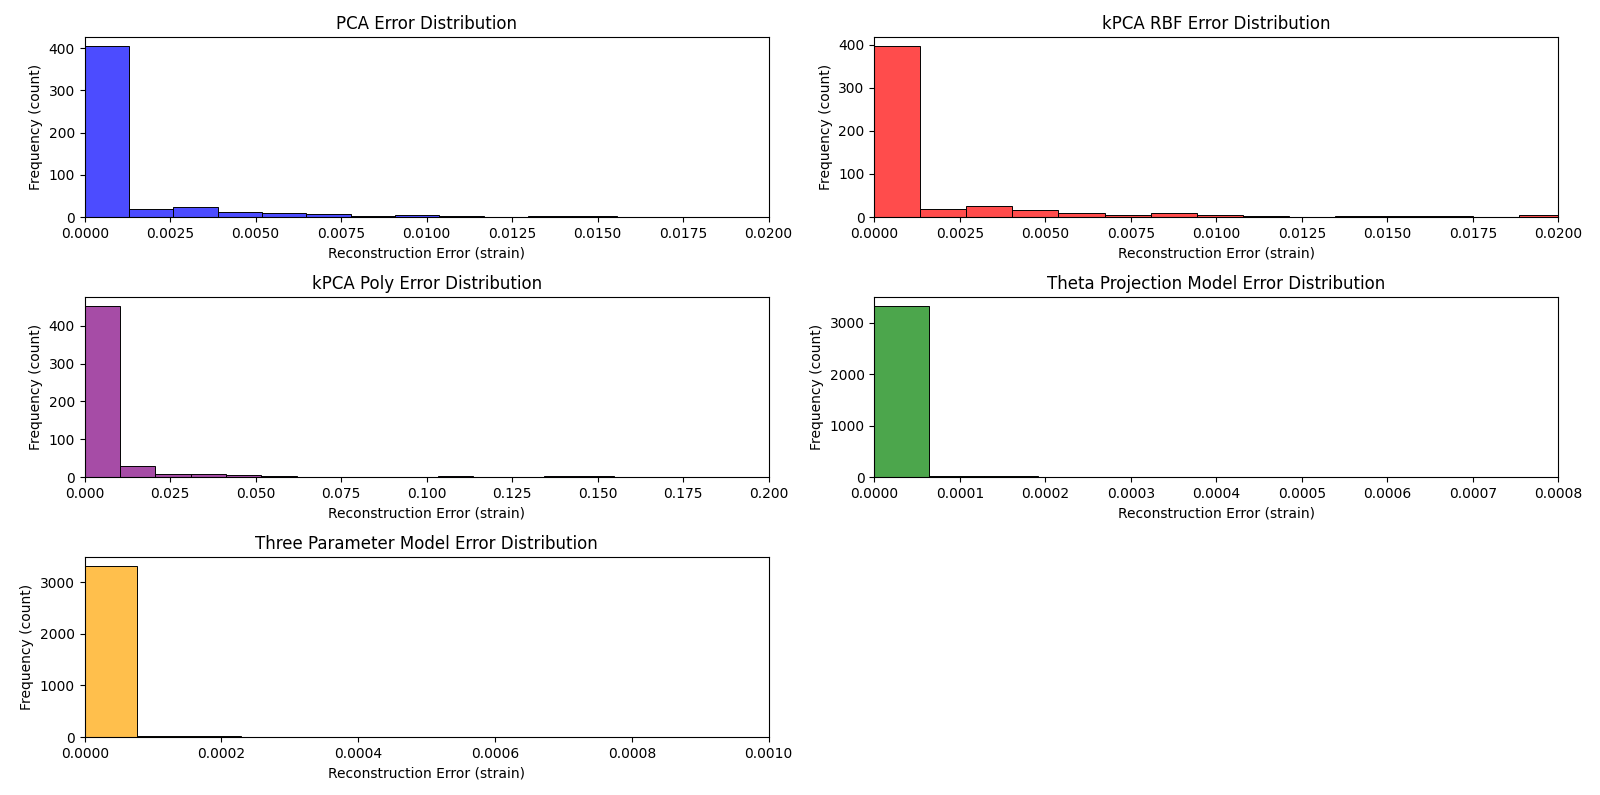
\includegraphics[width=1\textwidth]{figures/rmse_reconstruction_errors.png}
		\caption{RMSE histograms of different models.}
		\label{fig:rmse_reconstruction_errors}
	\end{figure}
	
	Figure~\ref{fig:min_creep_rate_error_hist} shows the histogram of minimum creep rate errors for the different models.
	\begin{figure}[H]
		\centering
		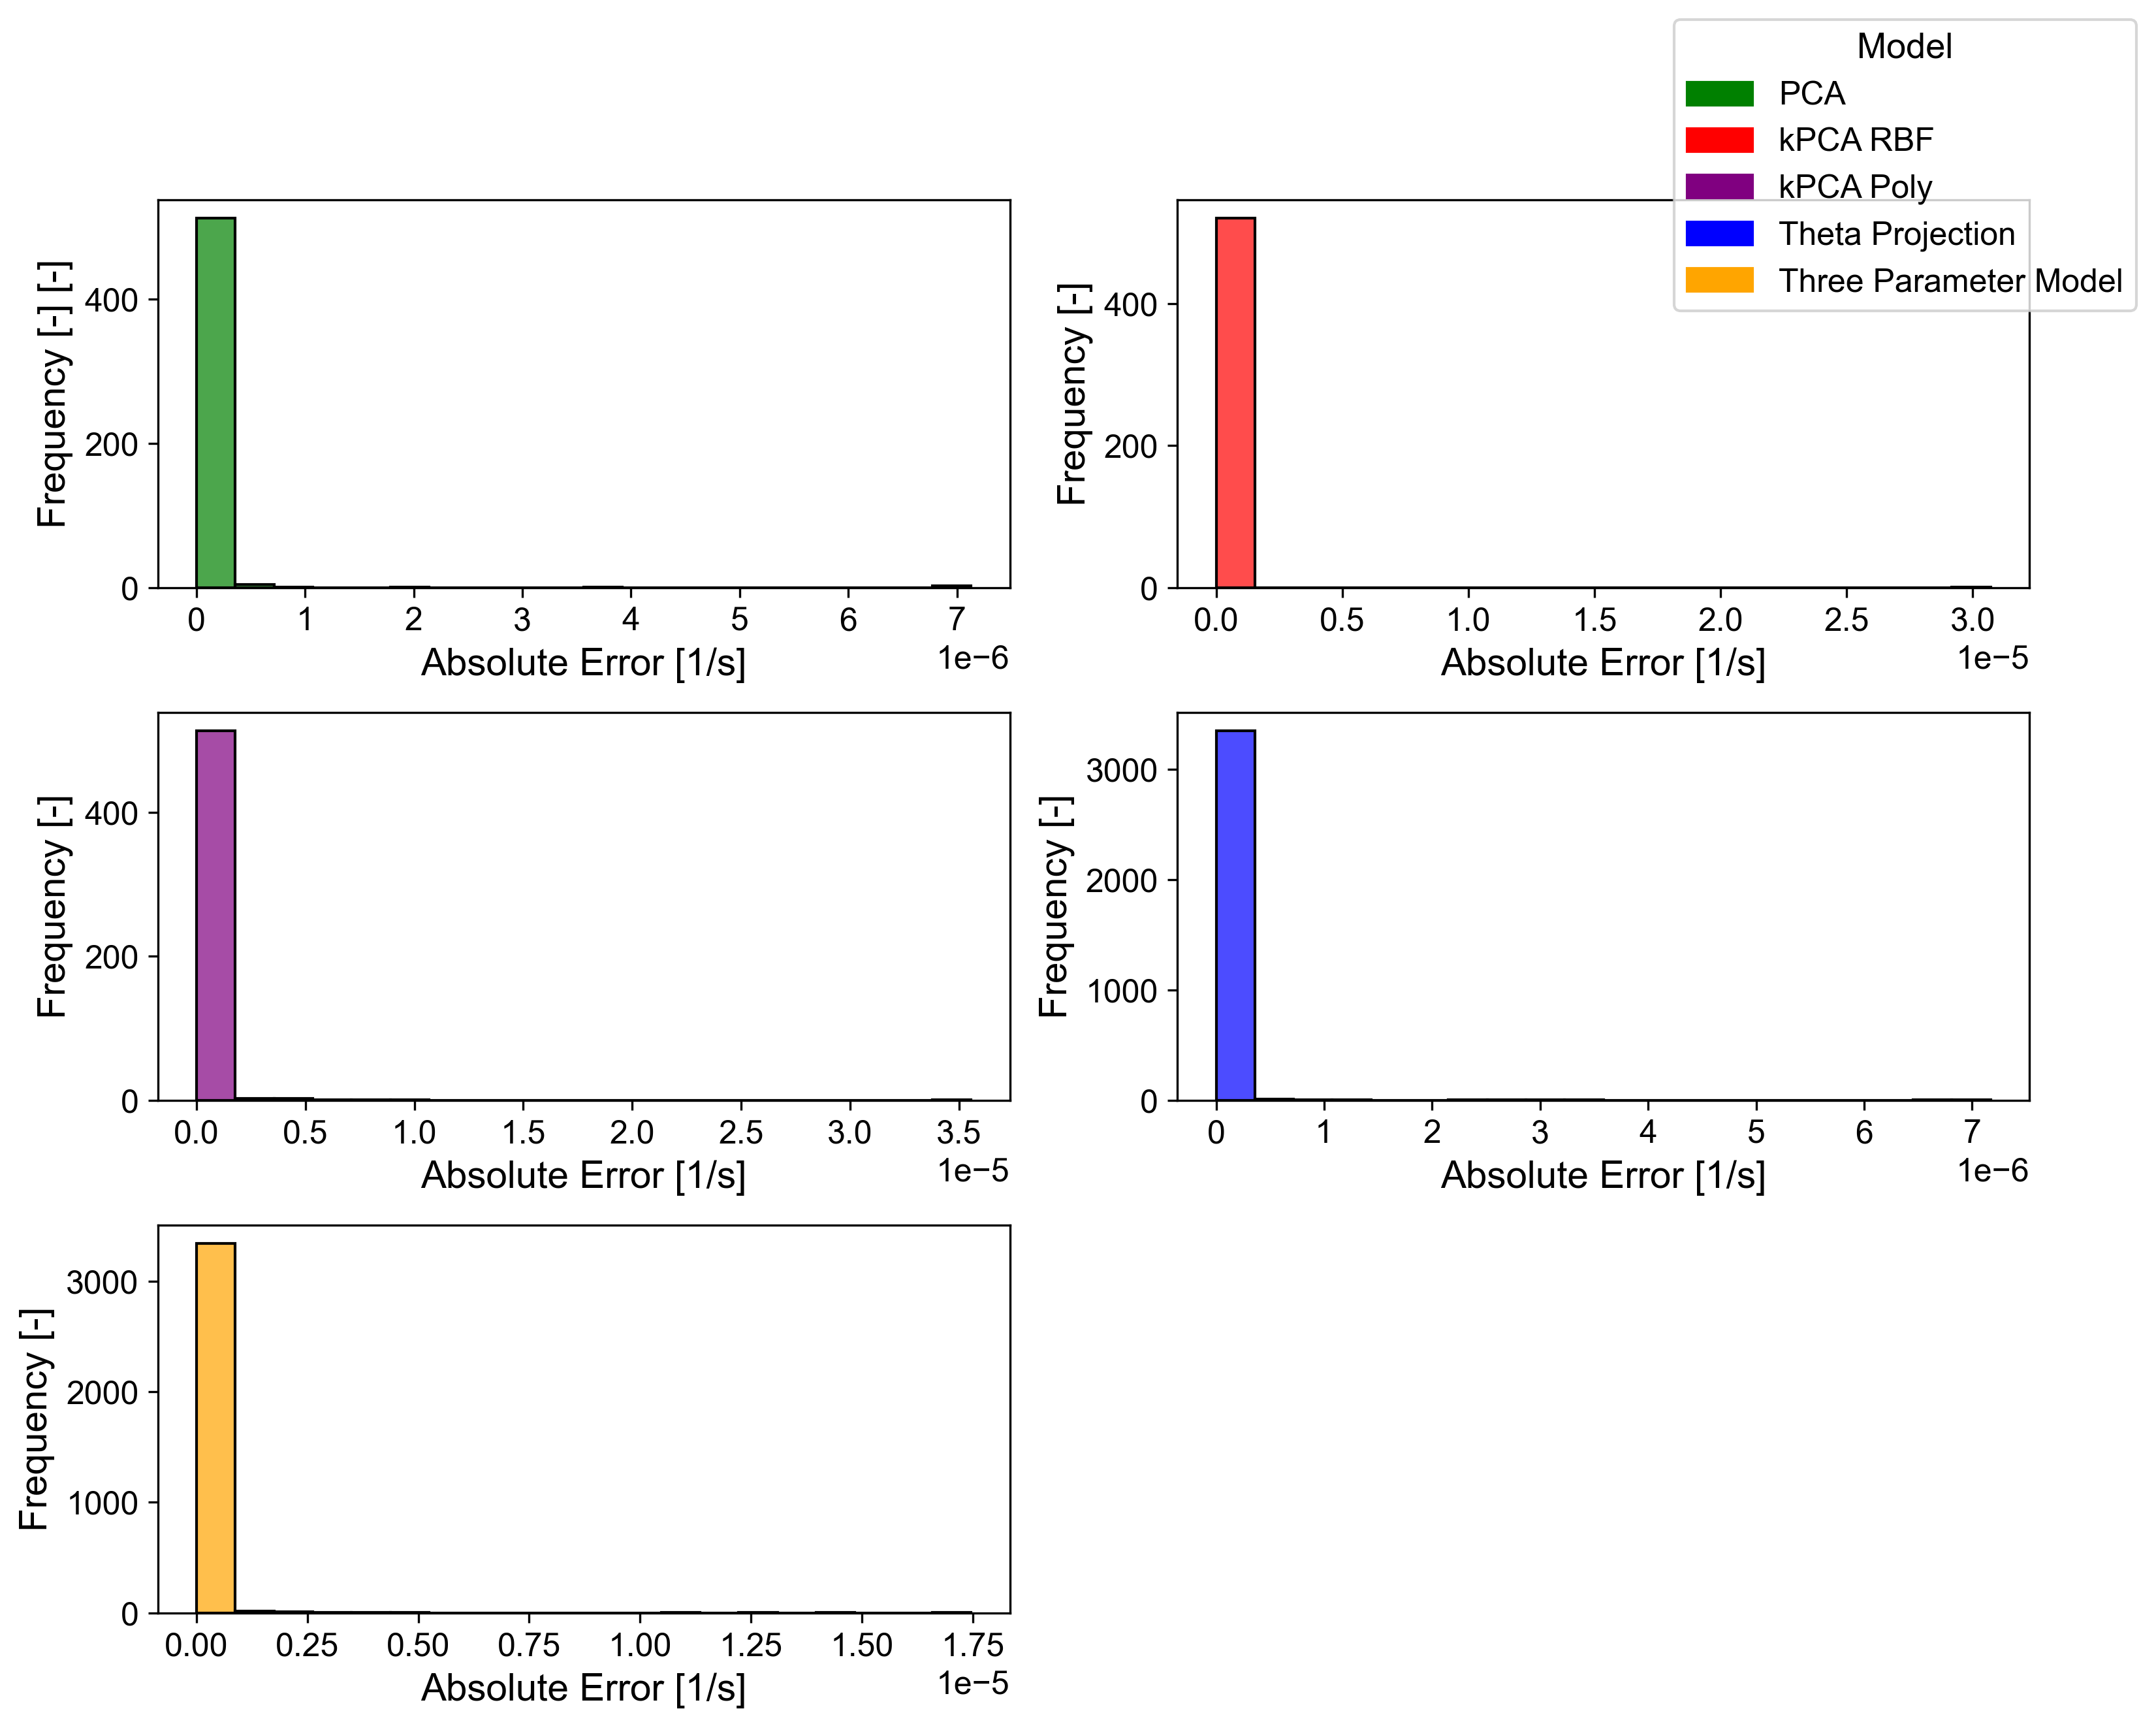
\includegraphics[width=1\textwidth]{figures/min_creep_rate_error_hist.png}
		\caption{Min. creep rate error histograms of different models.}
		\label{fig:min_creep_rate_error_hist}
	\end{figure}
	
	Figure~\ref{fig:fracture_time_error_hist} shows the histogram of time to rupture prediction for the different models.
	\begin{figure}[H]
		\centering
		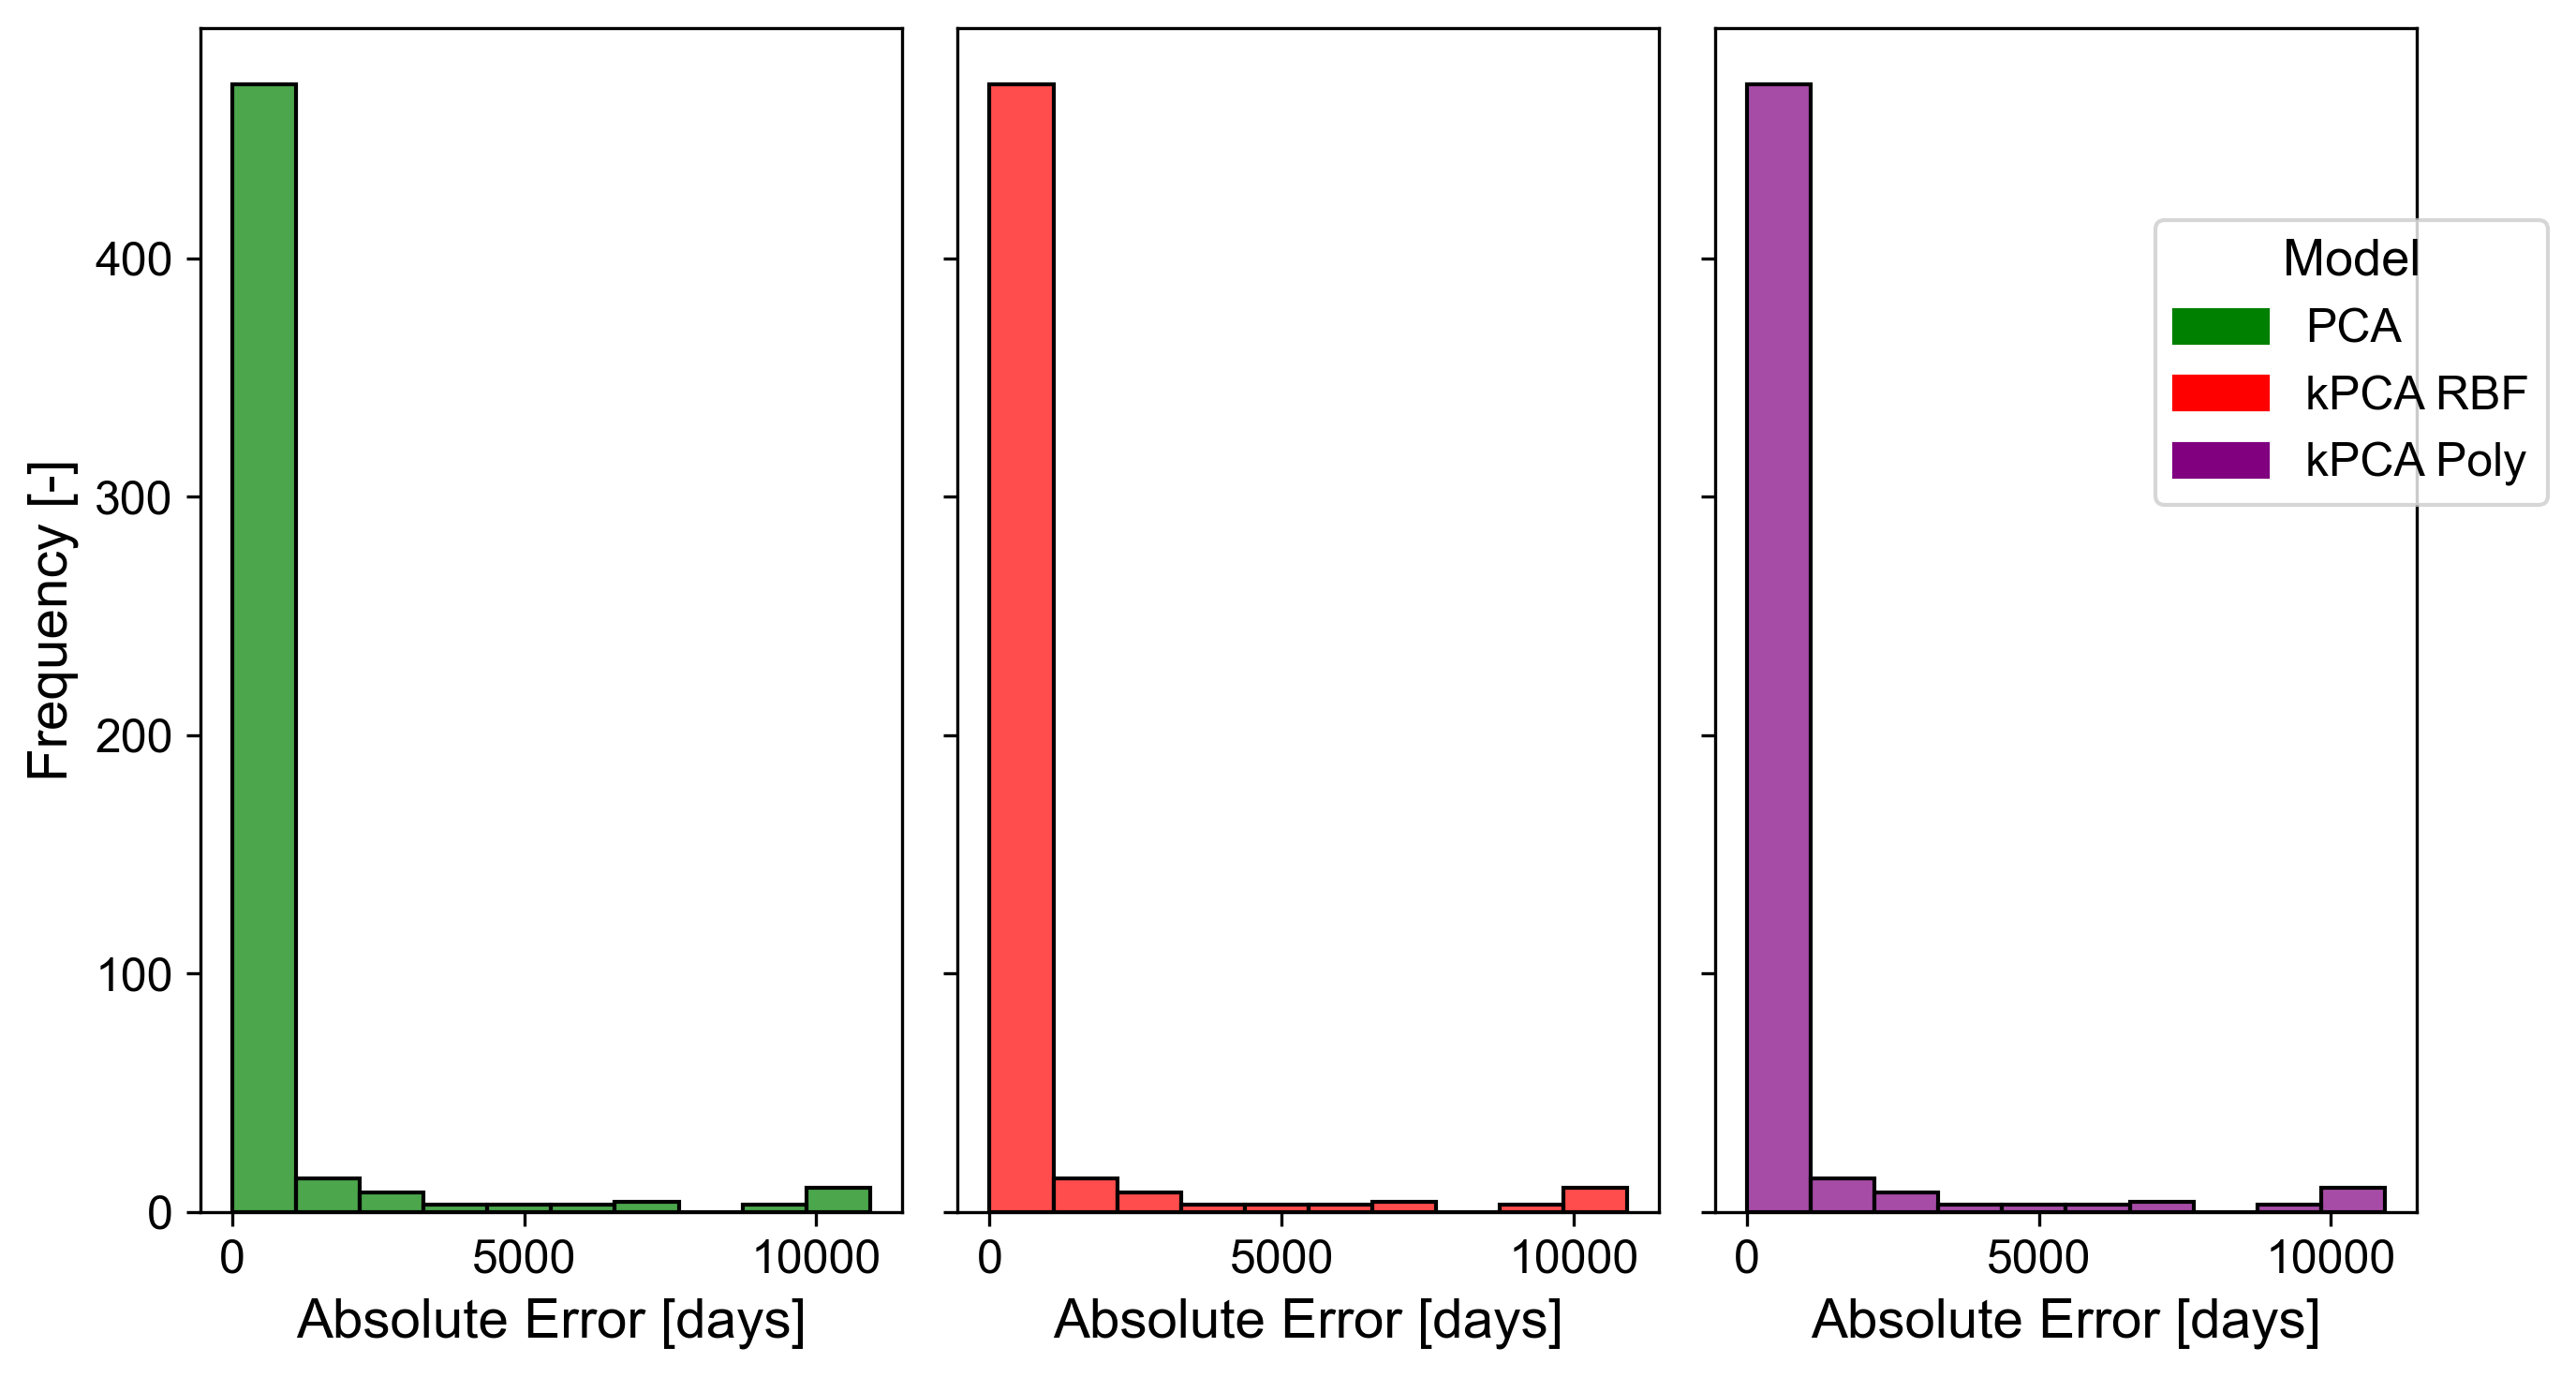
\includegraphics[width=0.9\textwidth]{figures/fracture_time_error_hist.png}
		\caption{Time to rupture prediction error histograms of different models.}
		\label{fig:fracture_time_error_hist}
	\end{figure}
	
	Table~\ref{tab:model_errors} shows the comparison between the different models already discussed in the section~\ref{Section::Results_CreepCurveRepresentations}.
	
	\begin{table}[ht]
		\centering
		\caption{Model Errors for the different Creep curve representations}
		\begin{tabularx}{\textwidth}{|X|X|X|X|X|X|}
			\hline
			\textbf{Metric} & \textbf{PCA} & \textbf{kPCA RBF} & \textbf{kPCA Poly} & \textbf{Theta Projection Model} & \textbf{Three Parameter Model} \\
			\hline
			\textbf{RMSE (Strain [-])} & 0.002683 & 0.002808 & 0.009904 & 0.000004 & 0.000007 \\
			\hline
			\textbf{Min. Creep Strain Rate} & $5.30 \times 10^{-8}$ & $6.22 \times 10^{-8}$ & $1.76 \times 10^{-7}$ & $1.54 \times 10^{-8}$ & $4.84 \times 10^{-8}$ \\
			\hline
			\textbf{Time to Rupture (days)} & 546 & 546 & 545 & - & - \\
			\hline
		\end{tabularx}
		\label{tab:model_errors}
	\end{table}
		
	\section{Active Learning Results}
	\label{Section::Results_AL}
	
	The active learning loop is run for 2000 iterations, selecting one new samples per iteration.	
	
	The Isolation Forest  classifier shows the convergence area of the material model parameters after the execution of the active learning loop. Figure~\ref{fig:pairwise_projections} shows the convergence of the pairwise projections mapping of the material model parameters.
	\begin{figure}[htbp]
		\centering
		\begin{tabular}{cccc}  % 4 columns
			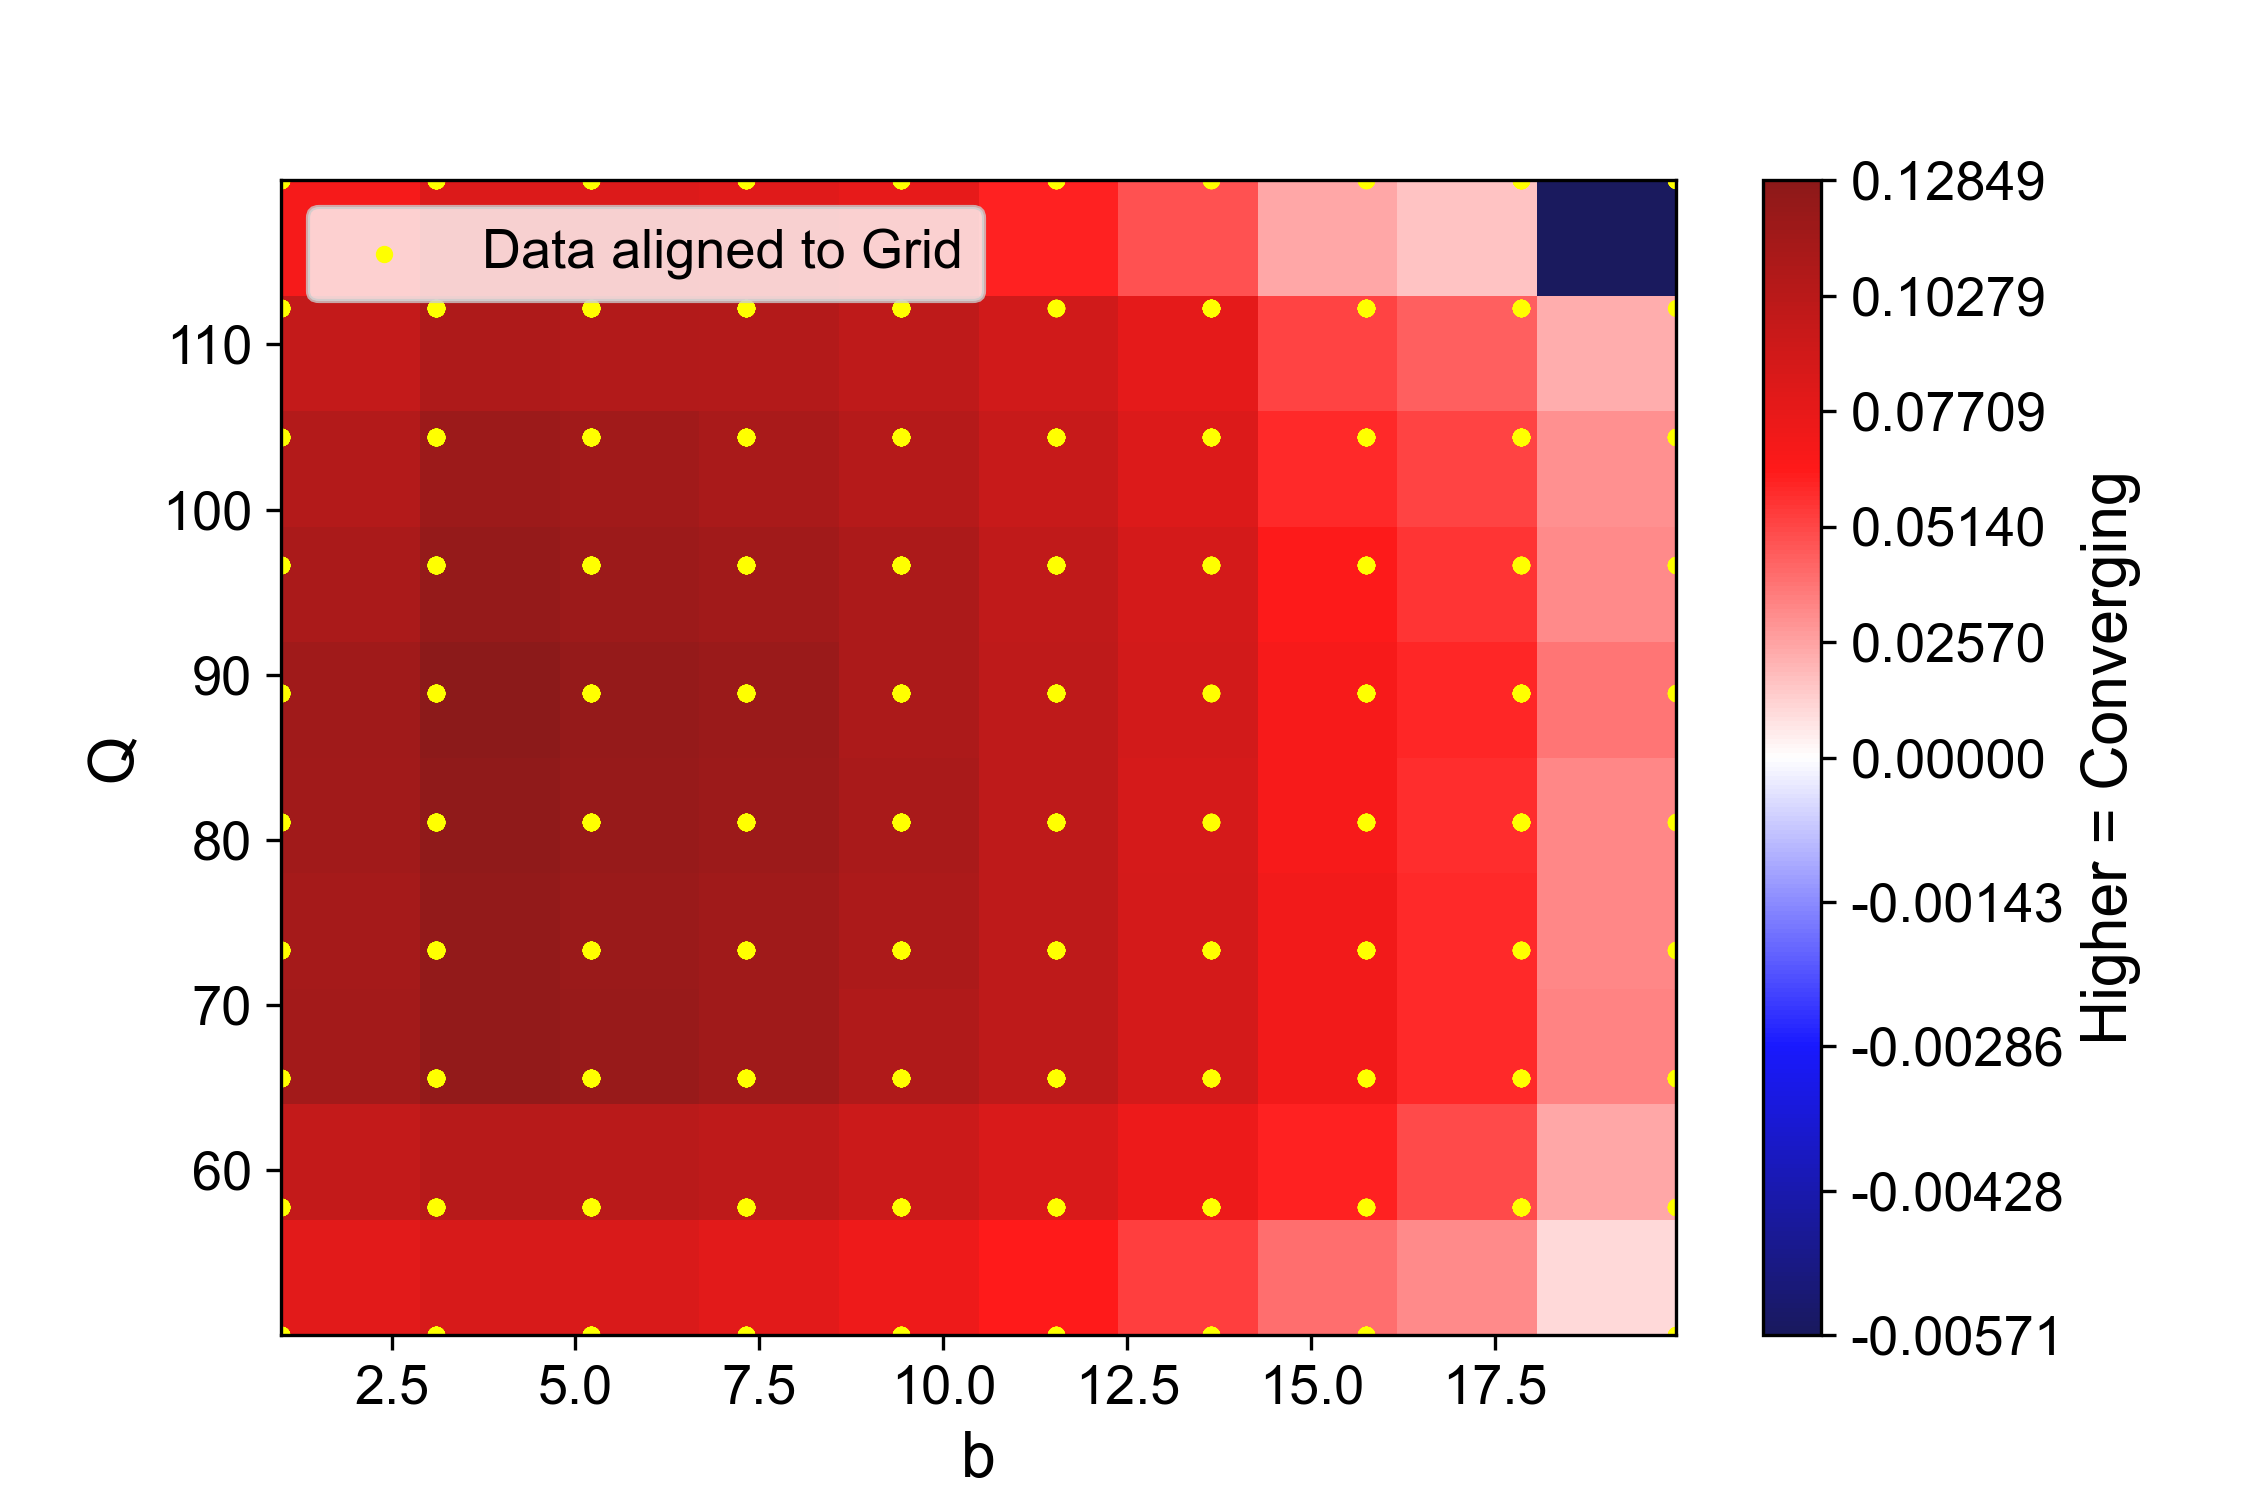
\includegraphics[width=0.32\textwidth]{figures/convergence/pairwise_projections_1.png} &
			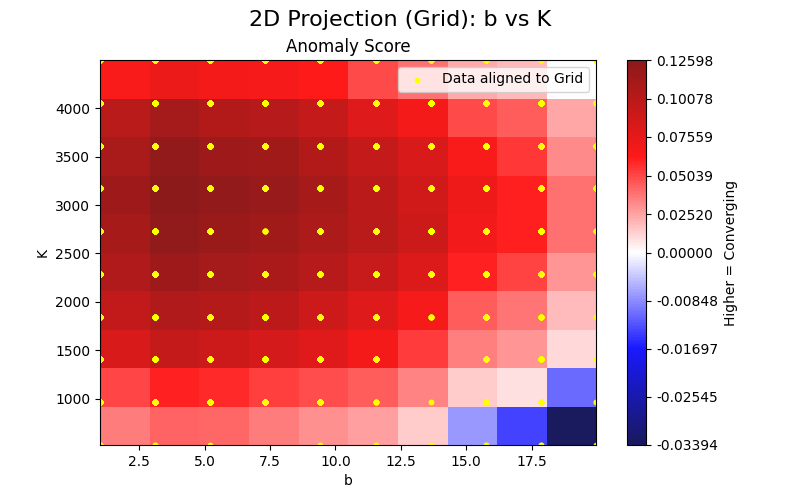
\includegraphics[width=0.32\textwidth]{figures/convergence/pairwise_projections_2.png} &
			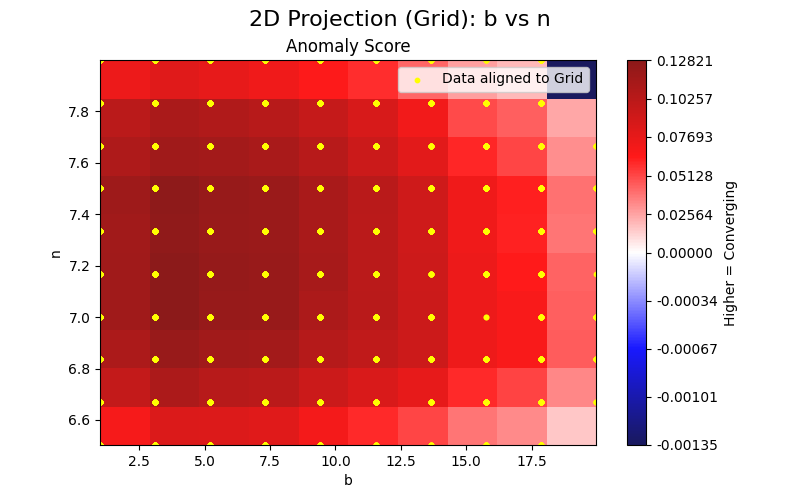
\includegraphics[width=0.32\textwidth]{figures/convergence/pairwise_projections_3.png} \\
			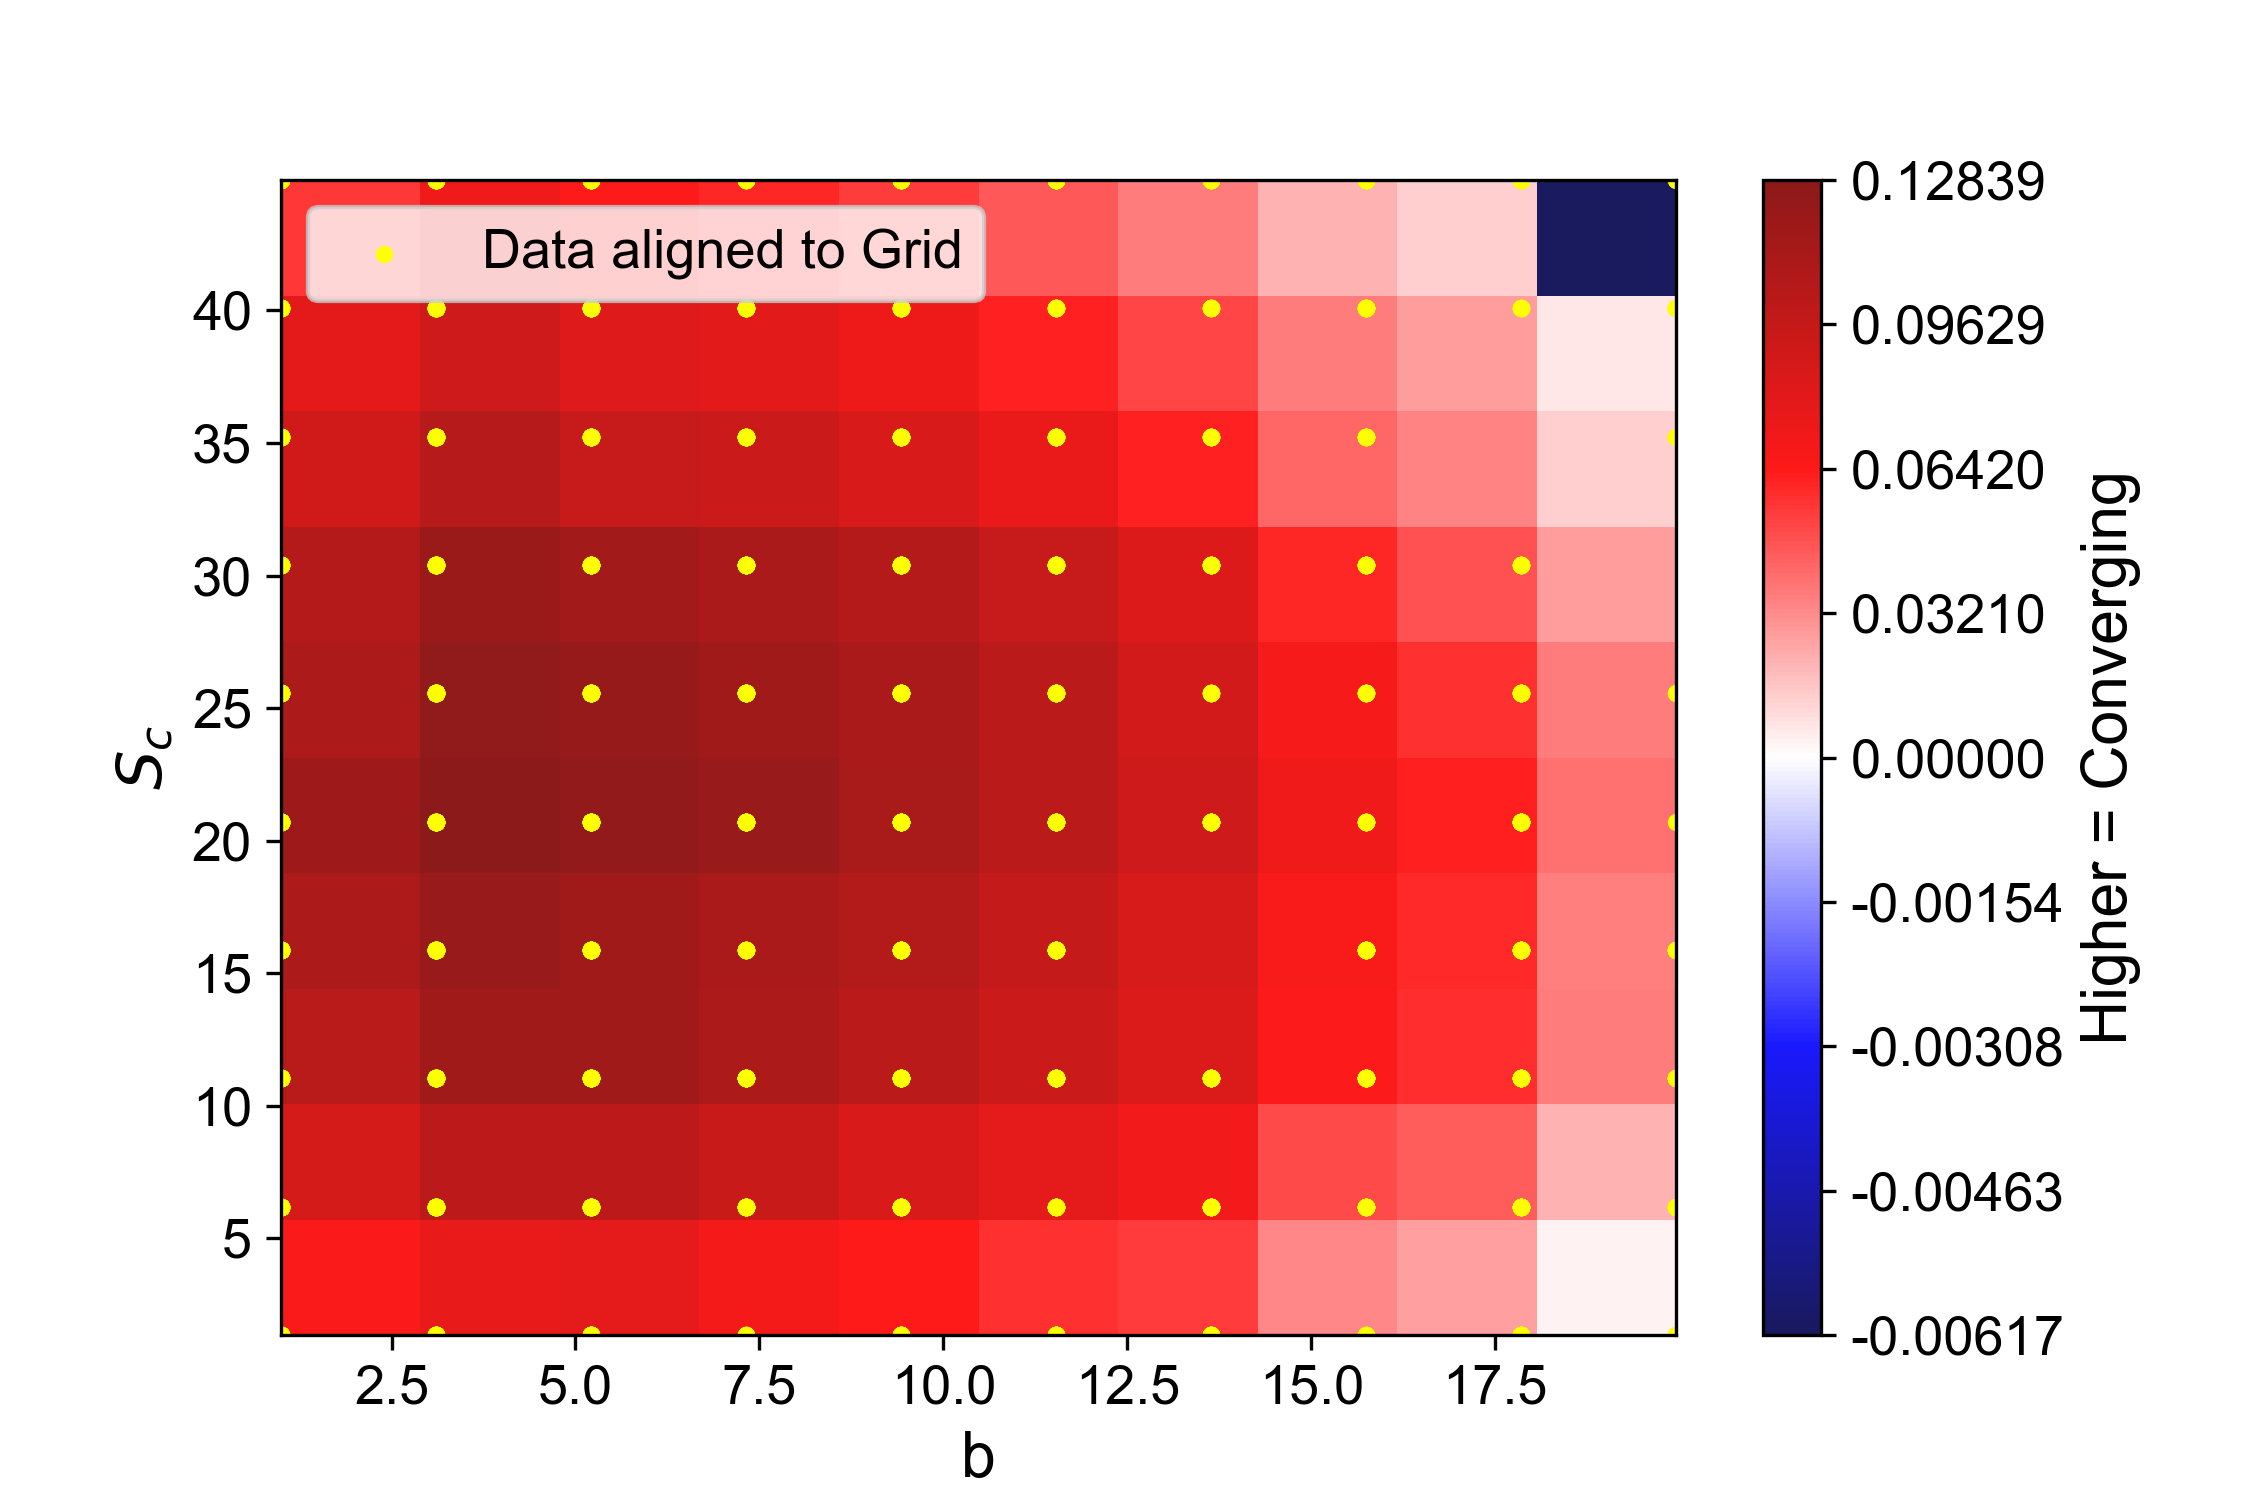
\includegraphics[width=0.32\textwidth]{figures/convergence/pairwise_projections_4.png} &
			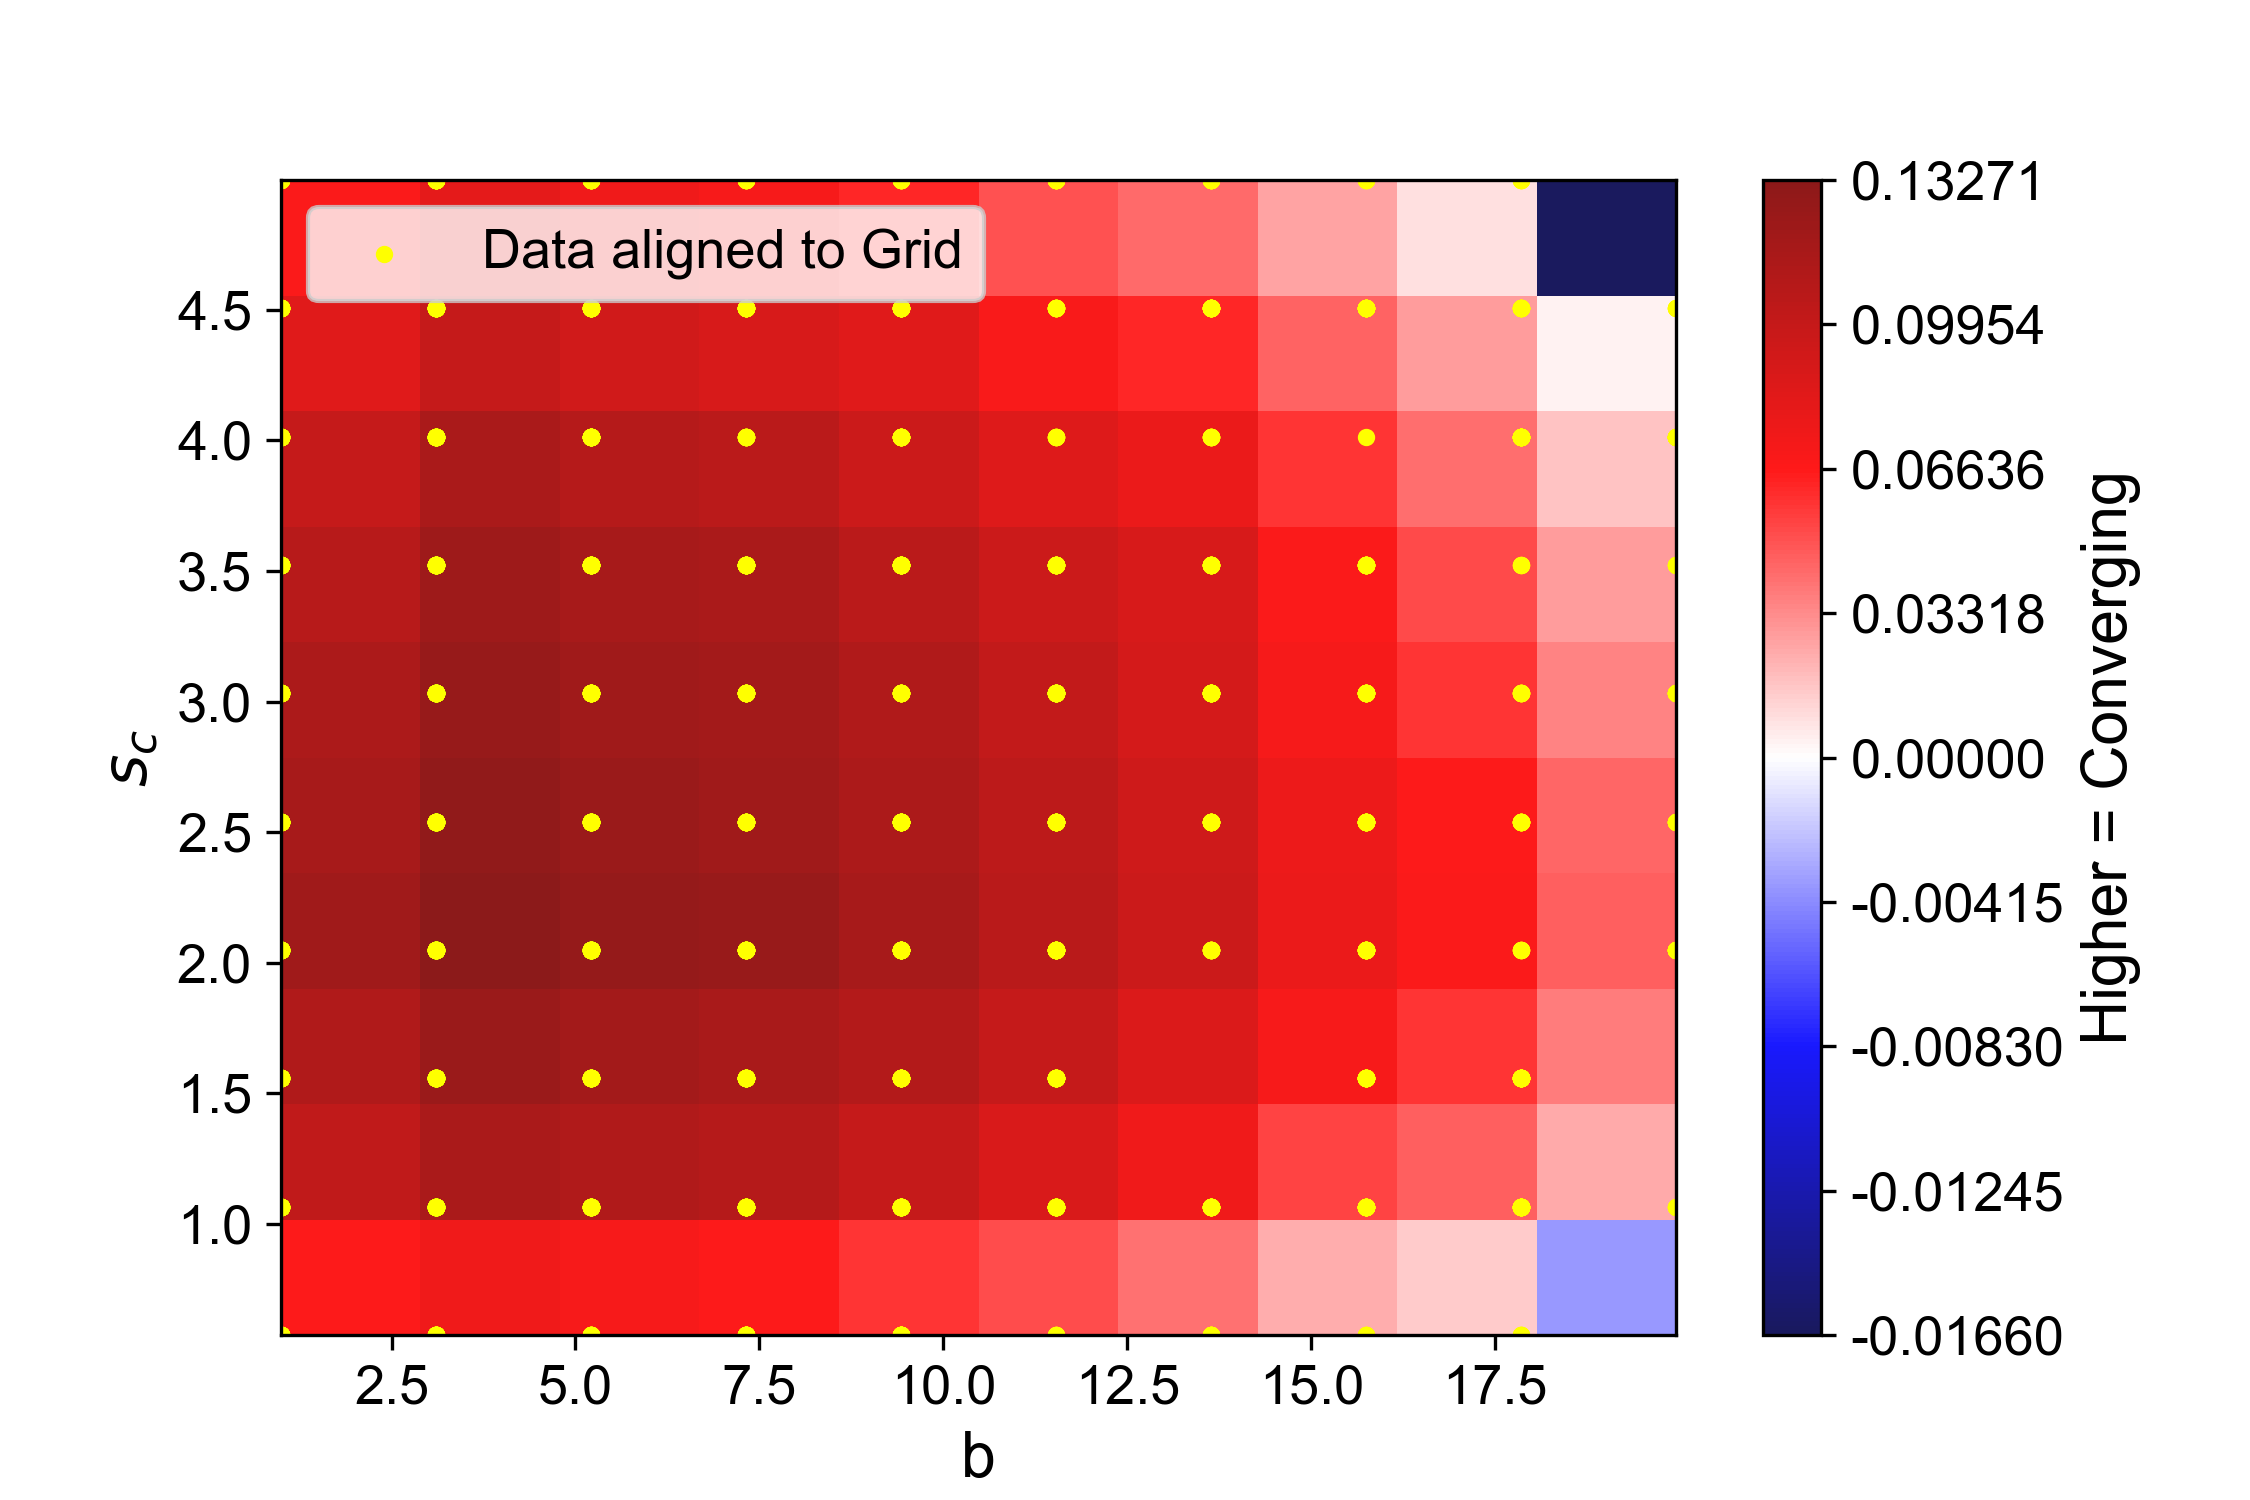
\includegraphics[width=0.32\textwidth]{figures/convergence/pairwise_projections_5.png} &
			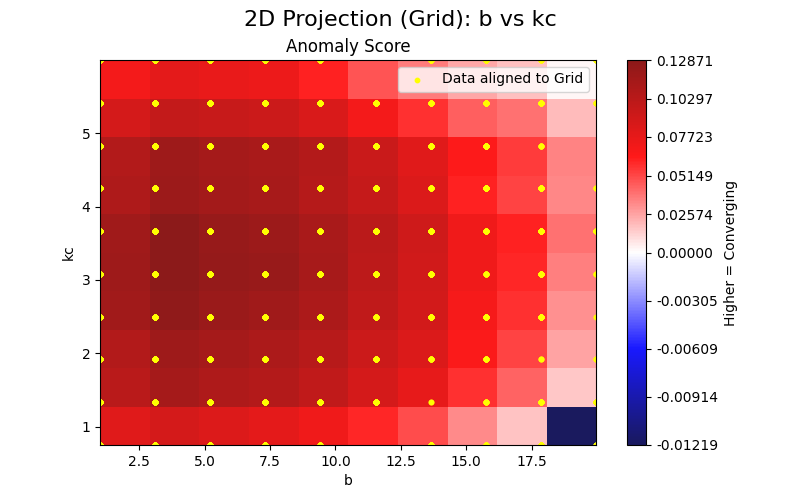
\includegraphics[width=0.32\textwidth]{figures/convergence/pairwise_projections_6.png} \\
			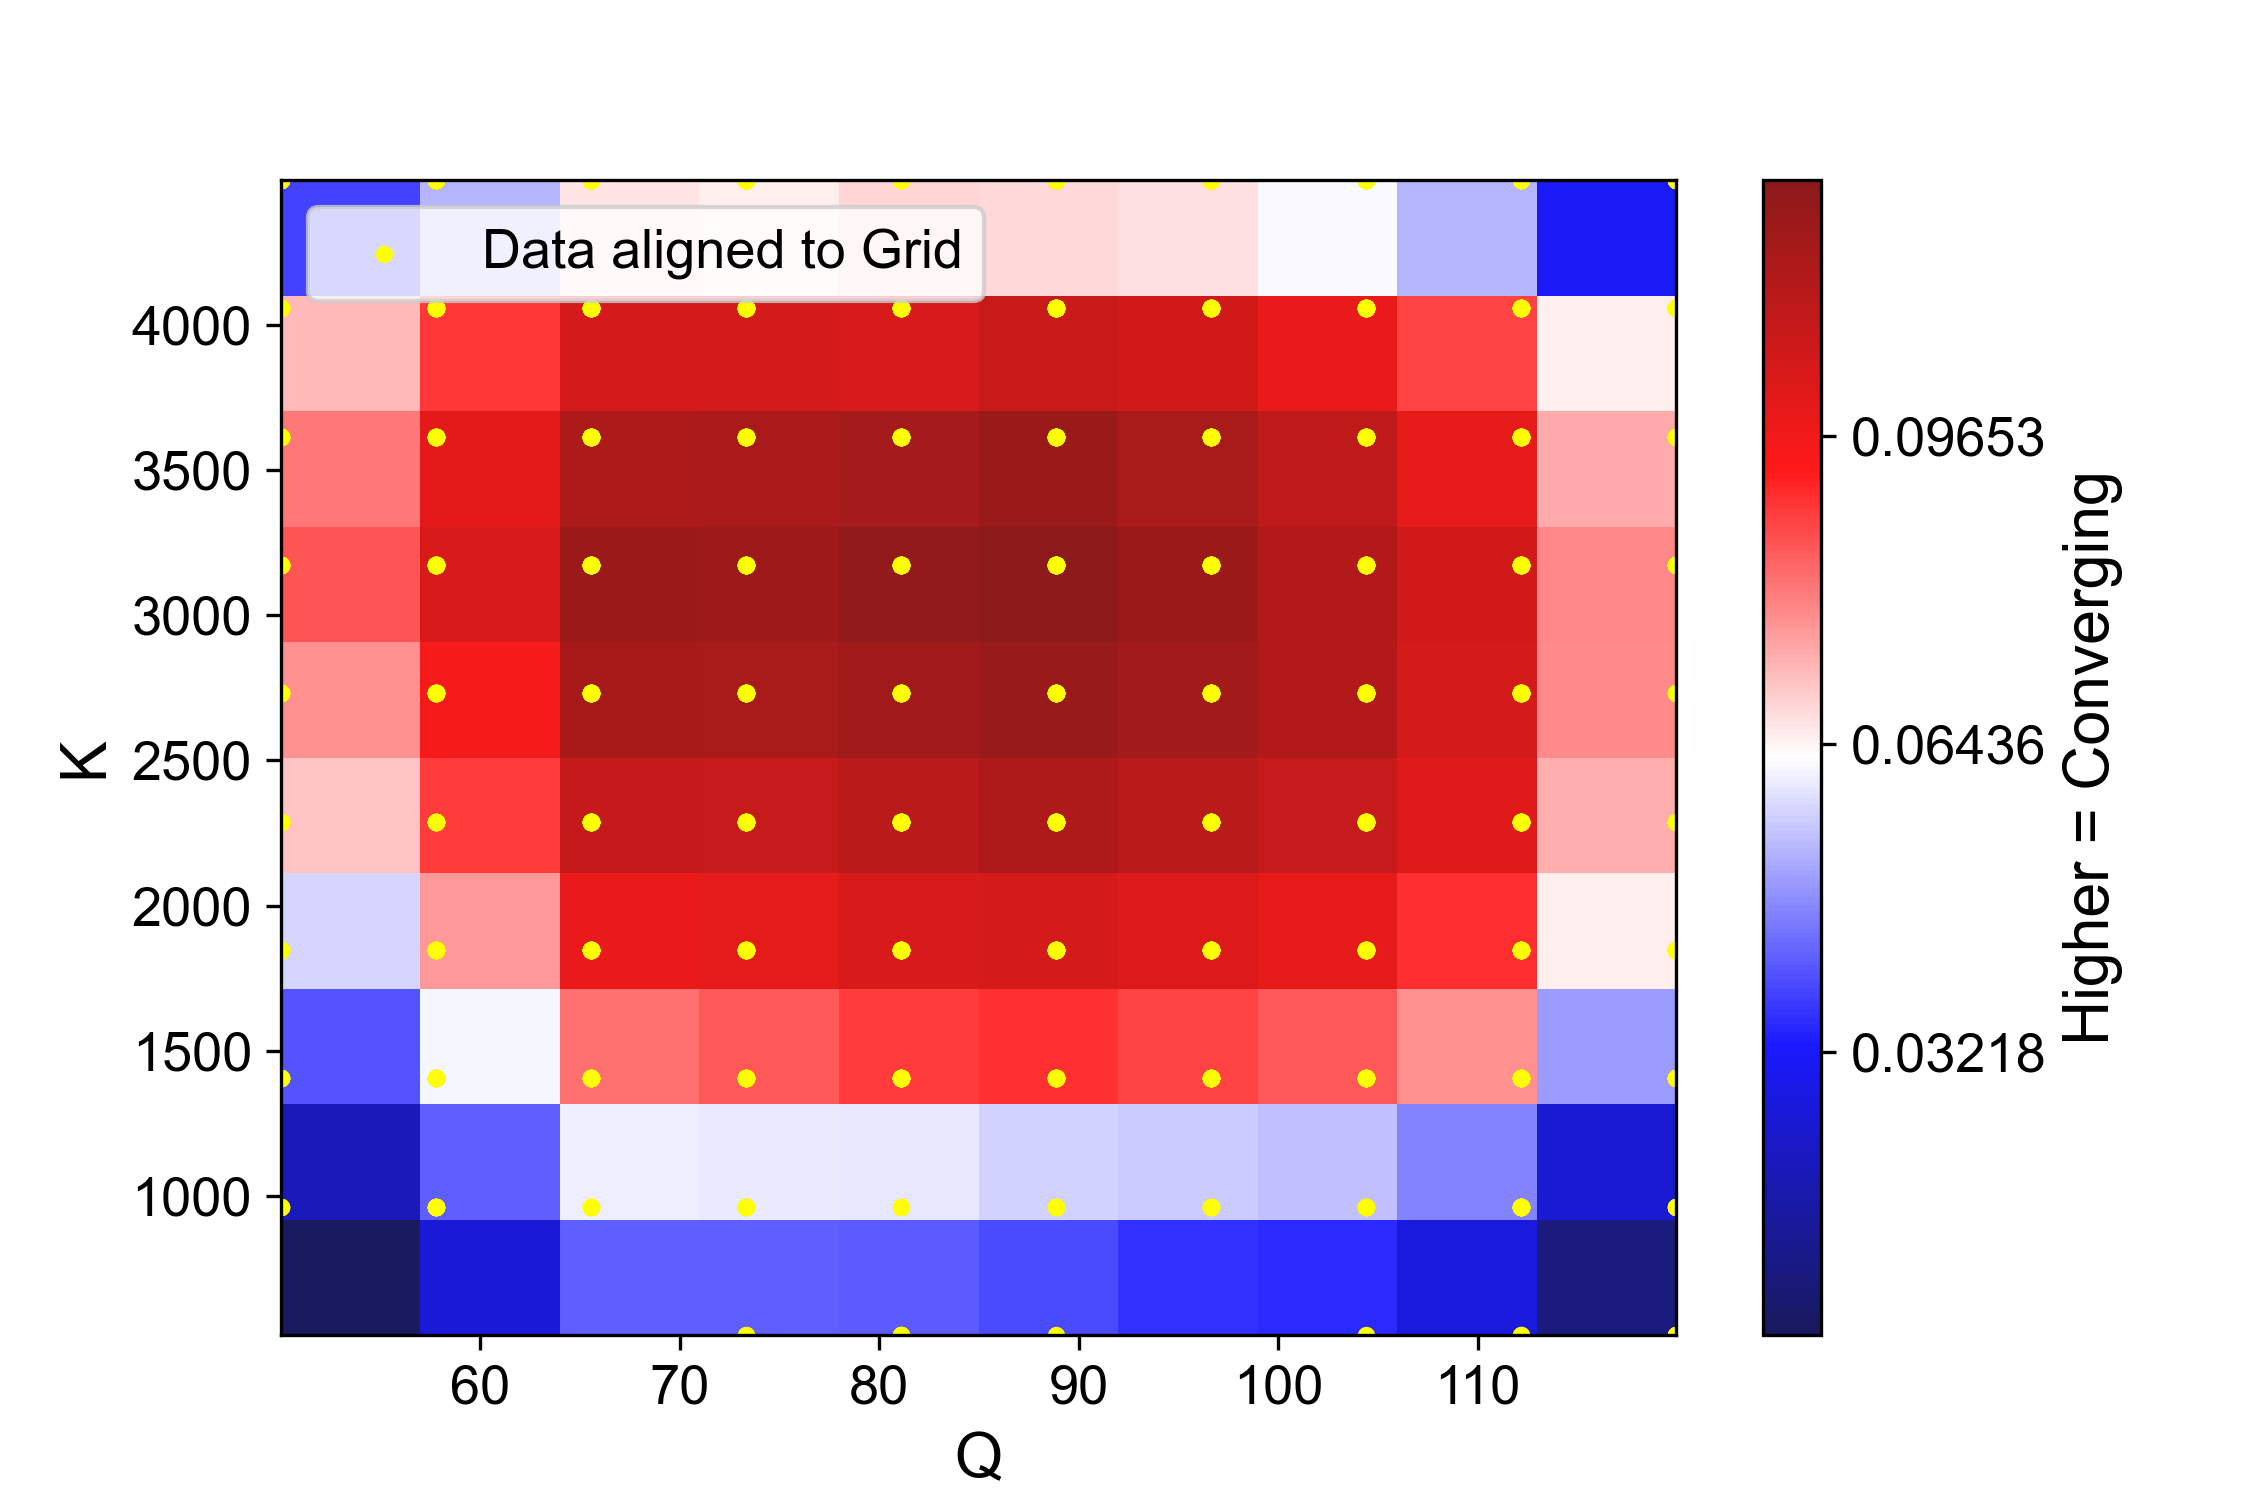
\includegraphics[width=0.32\textwidth]{figures/convergence/pairwise_projections_7.png} &
			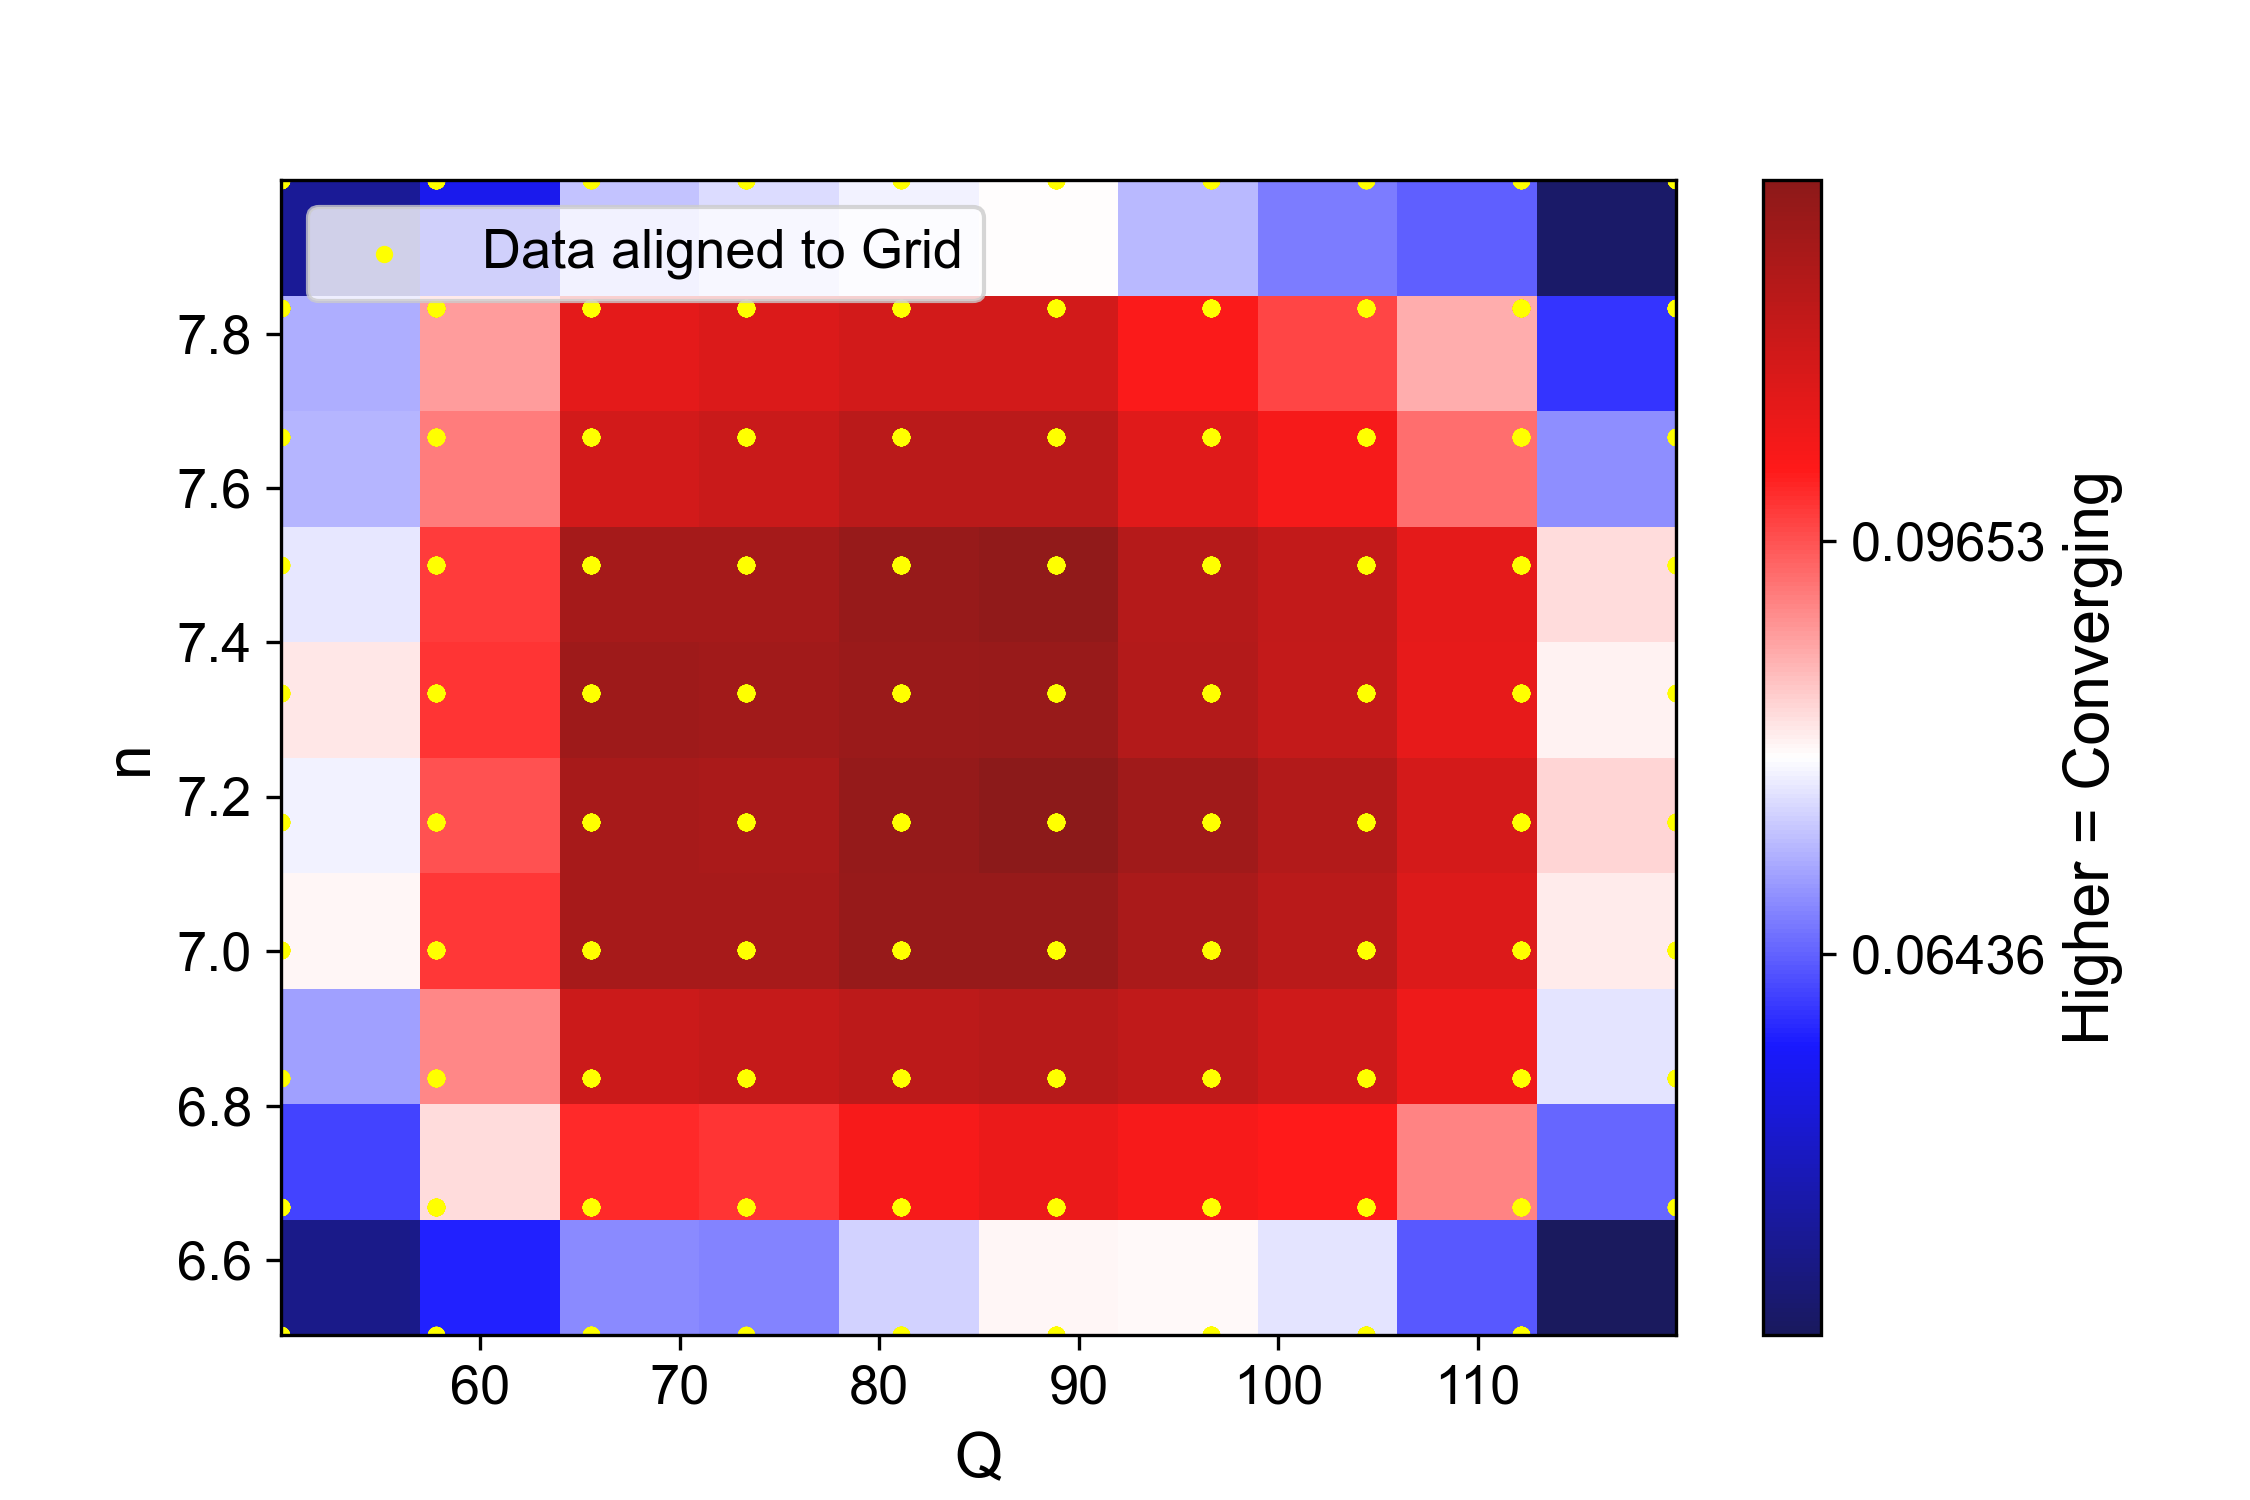
\includegraphics[width=0.32\textwidth]{figures/convergence/pairwise_projections_8.png} &
			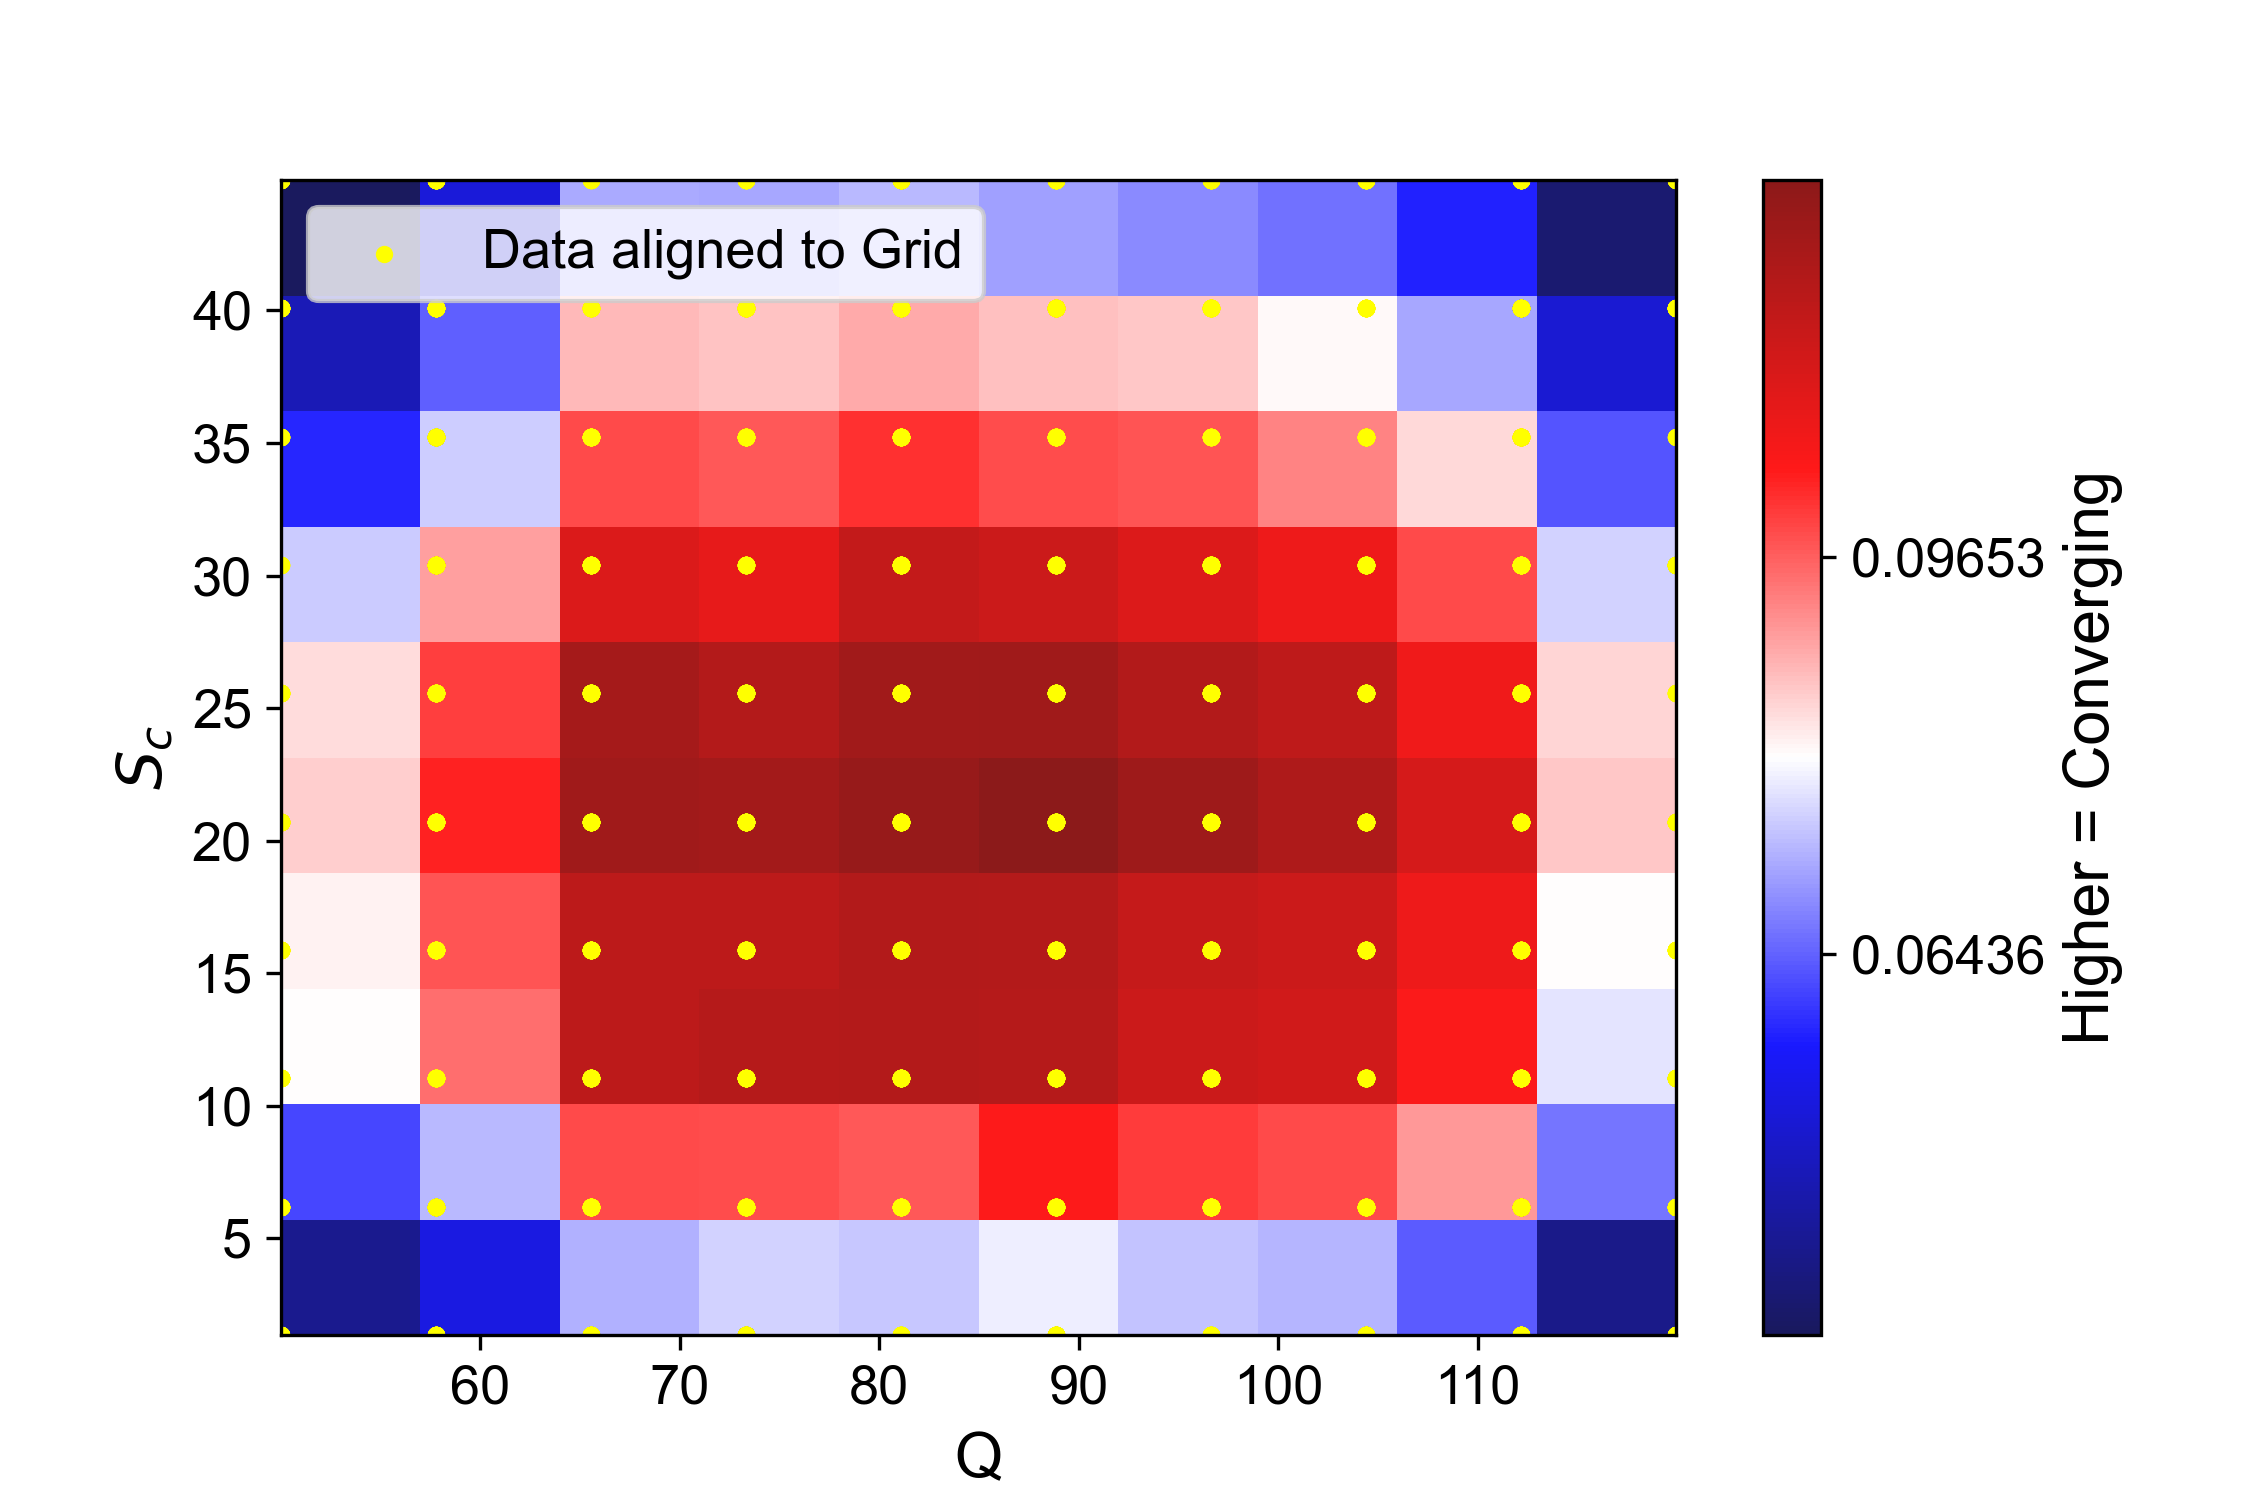
\includegraphics[width=0.32\textwidth]{figures/convergence/pairwise_projections_9.png} \\
			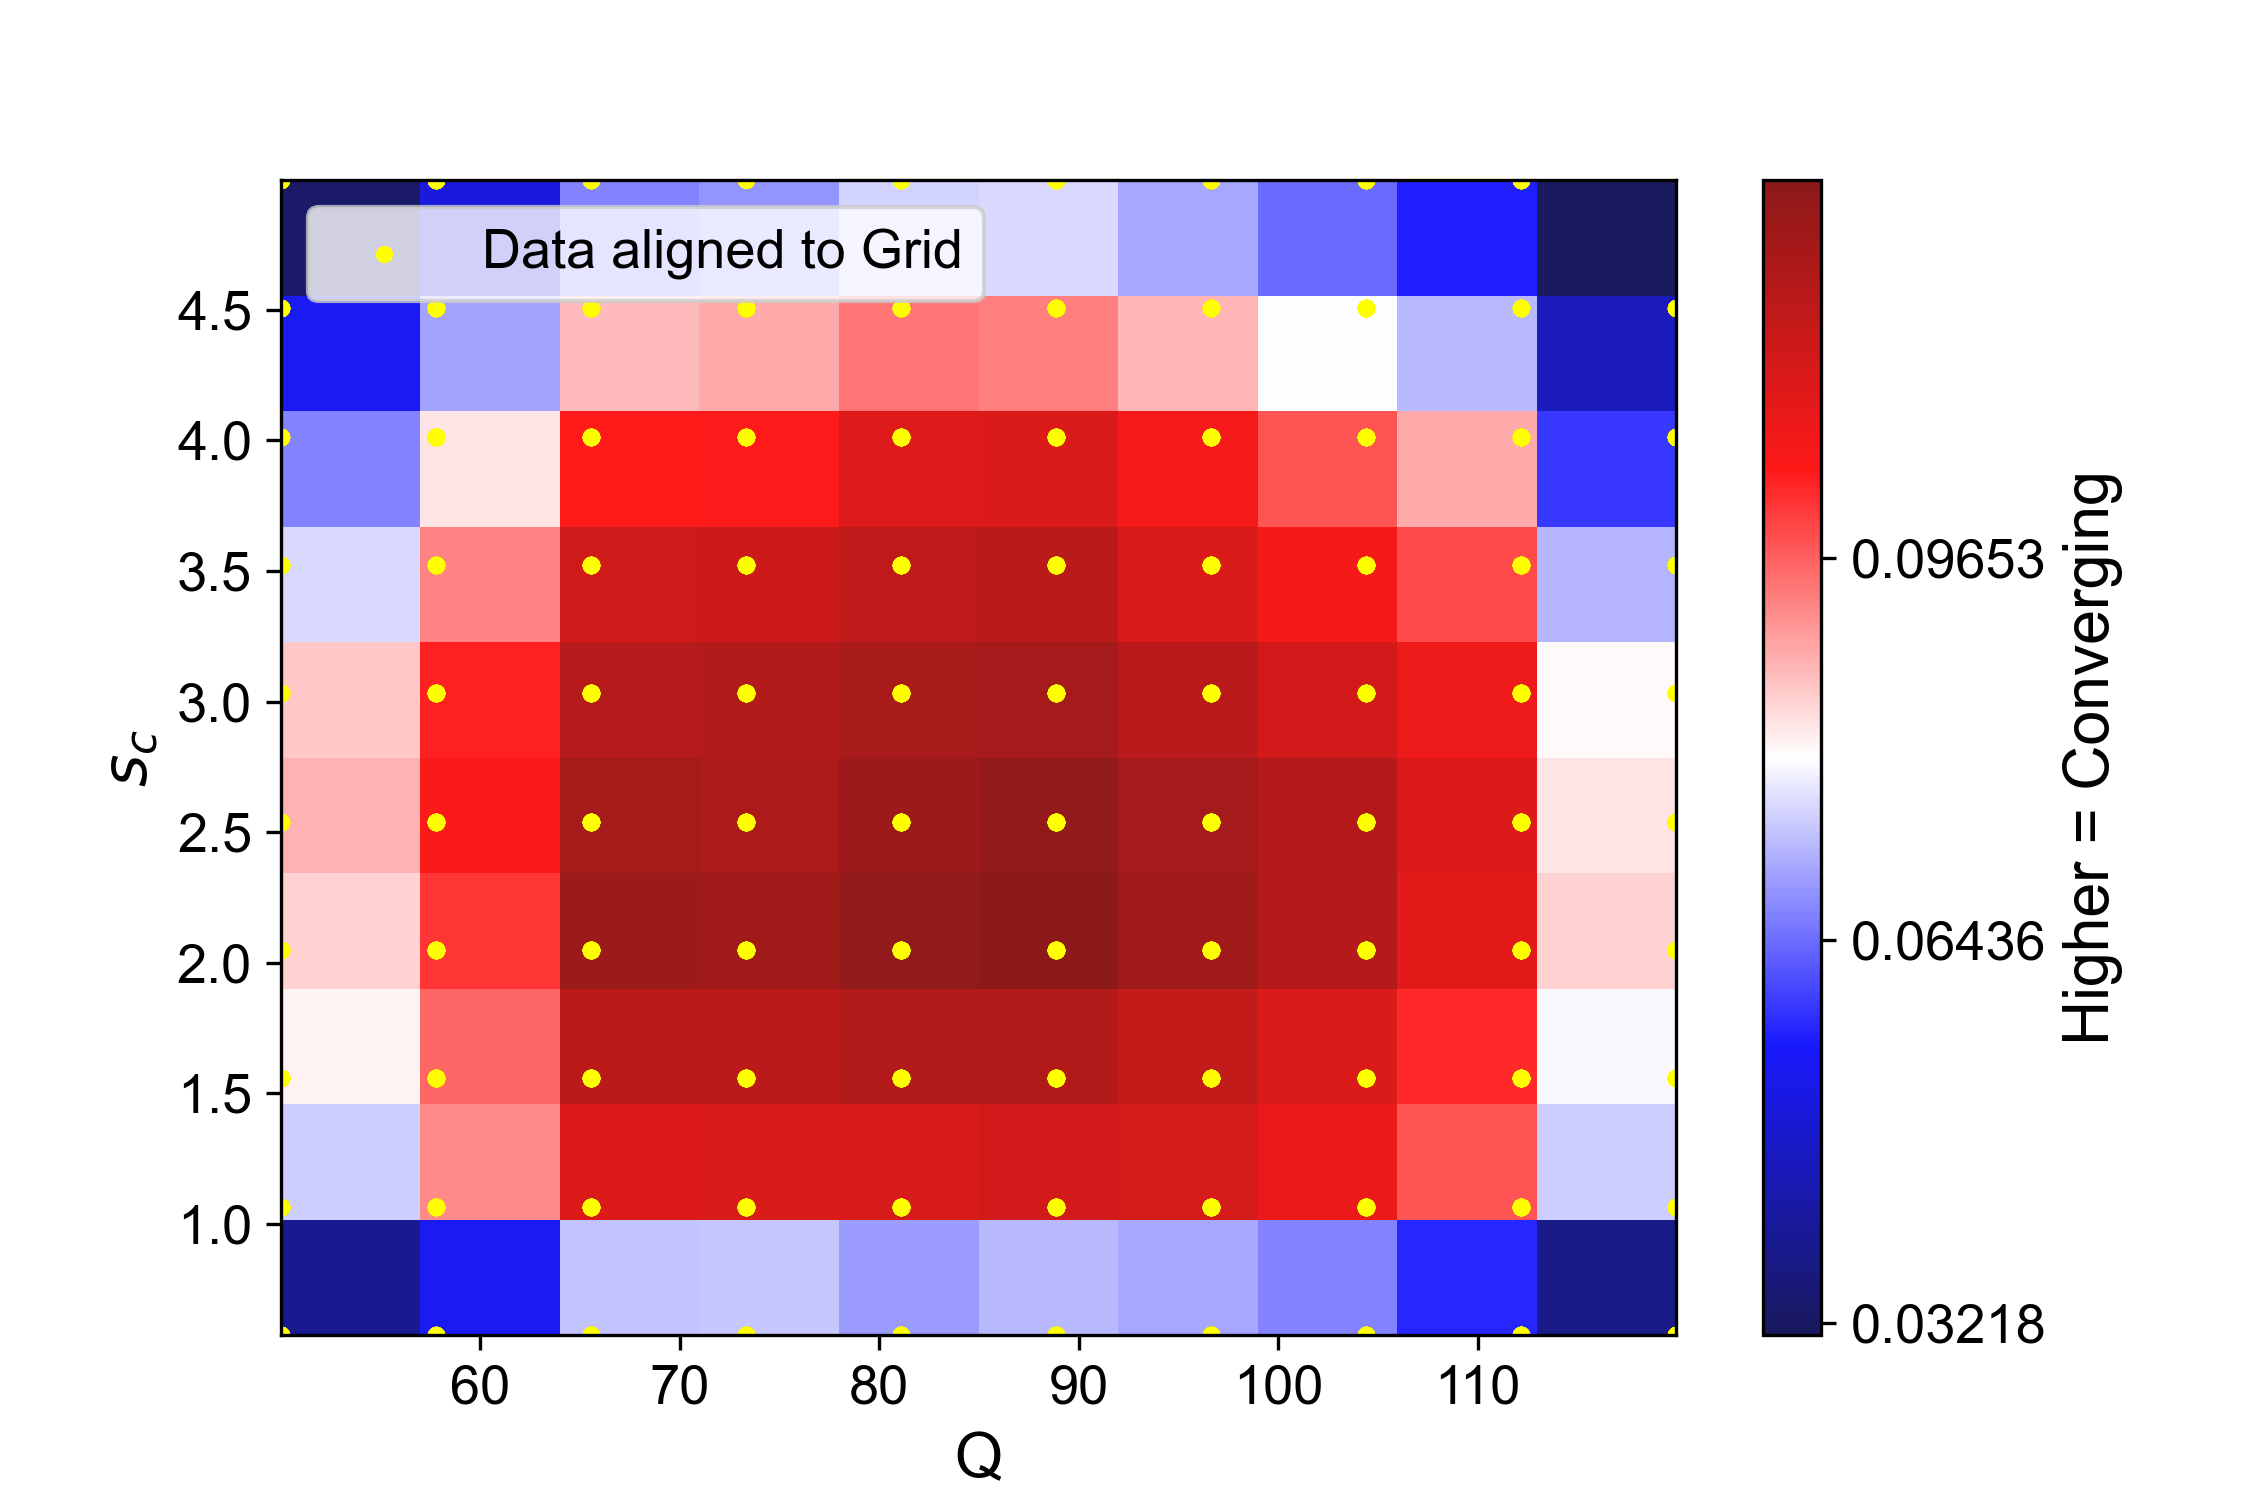
\includegraphics[width=0.32\textwidth]{figures/convergence/pairwise_projections_10.png} &
			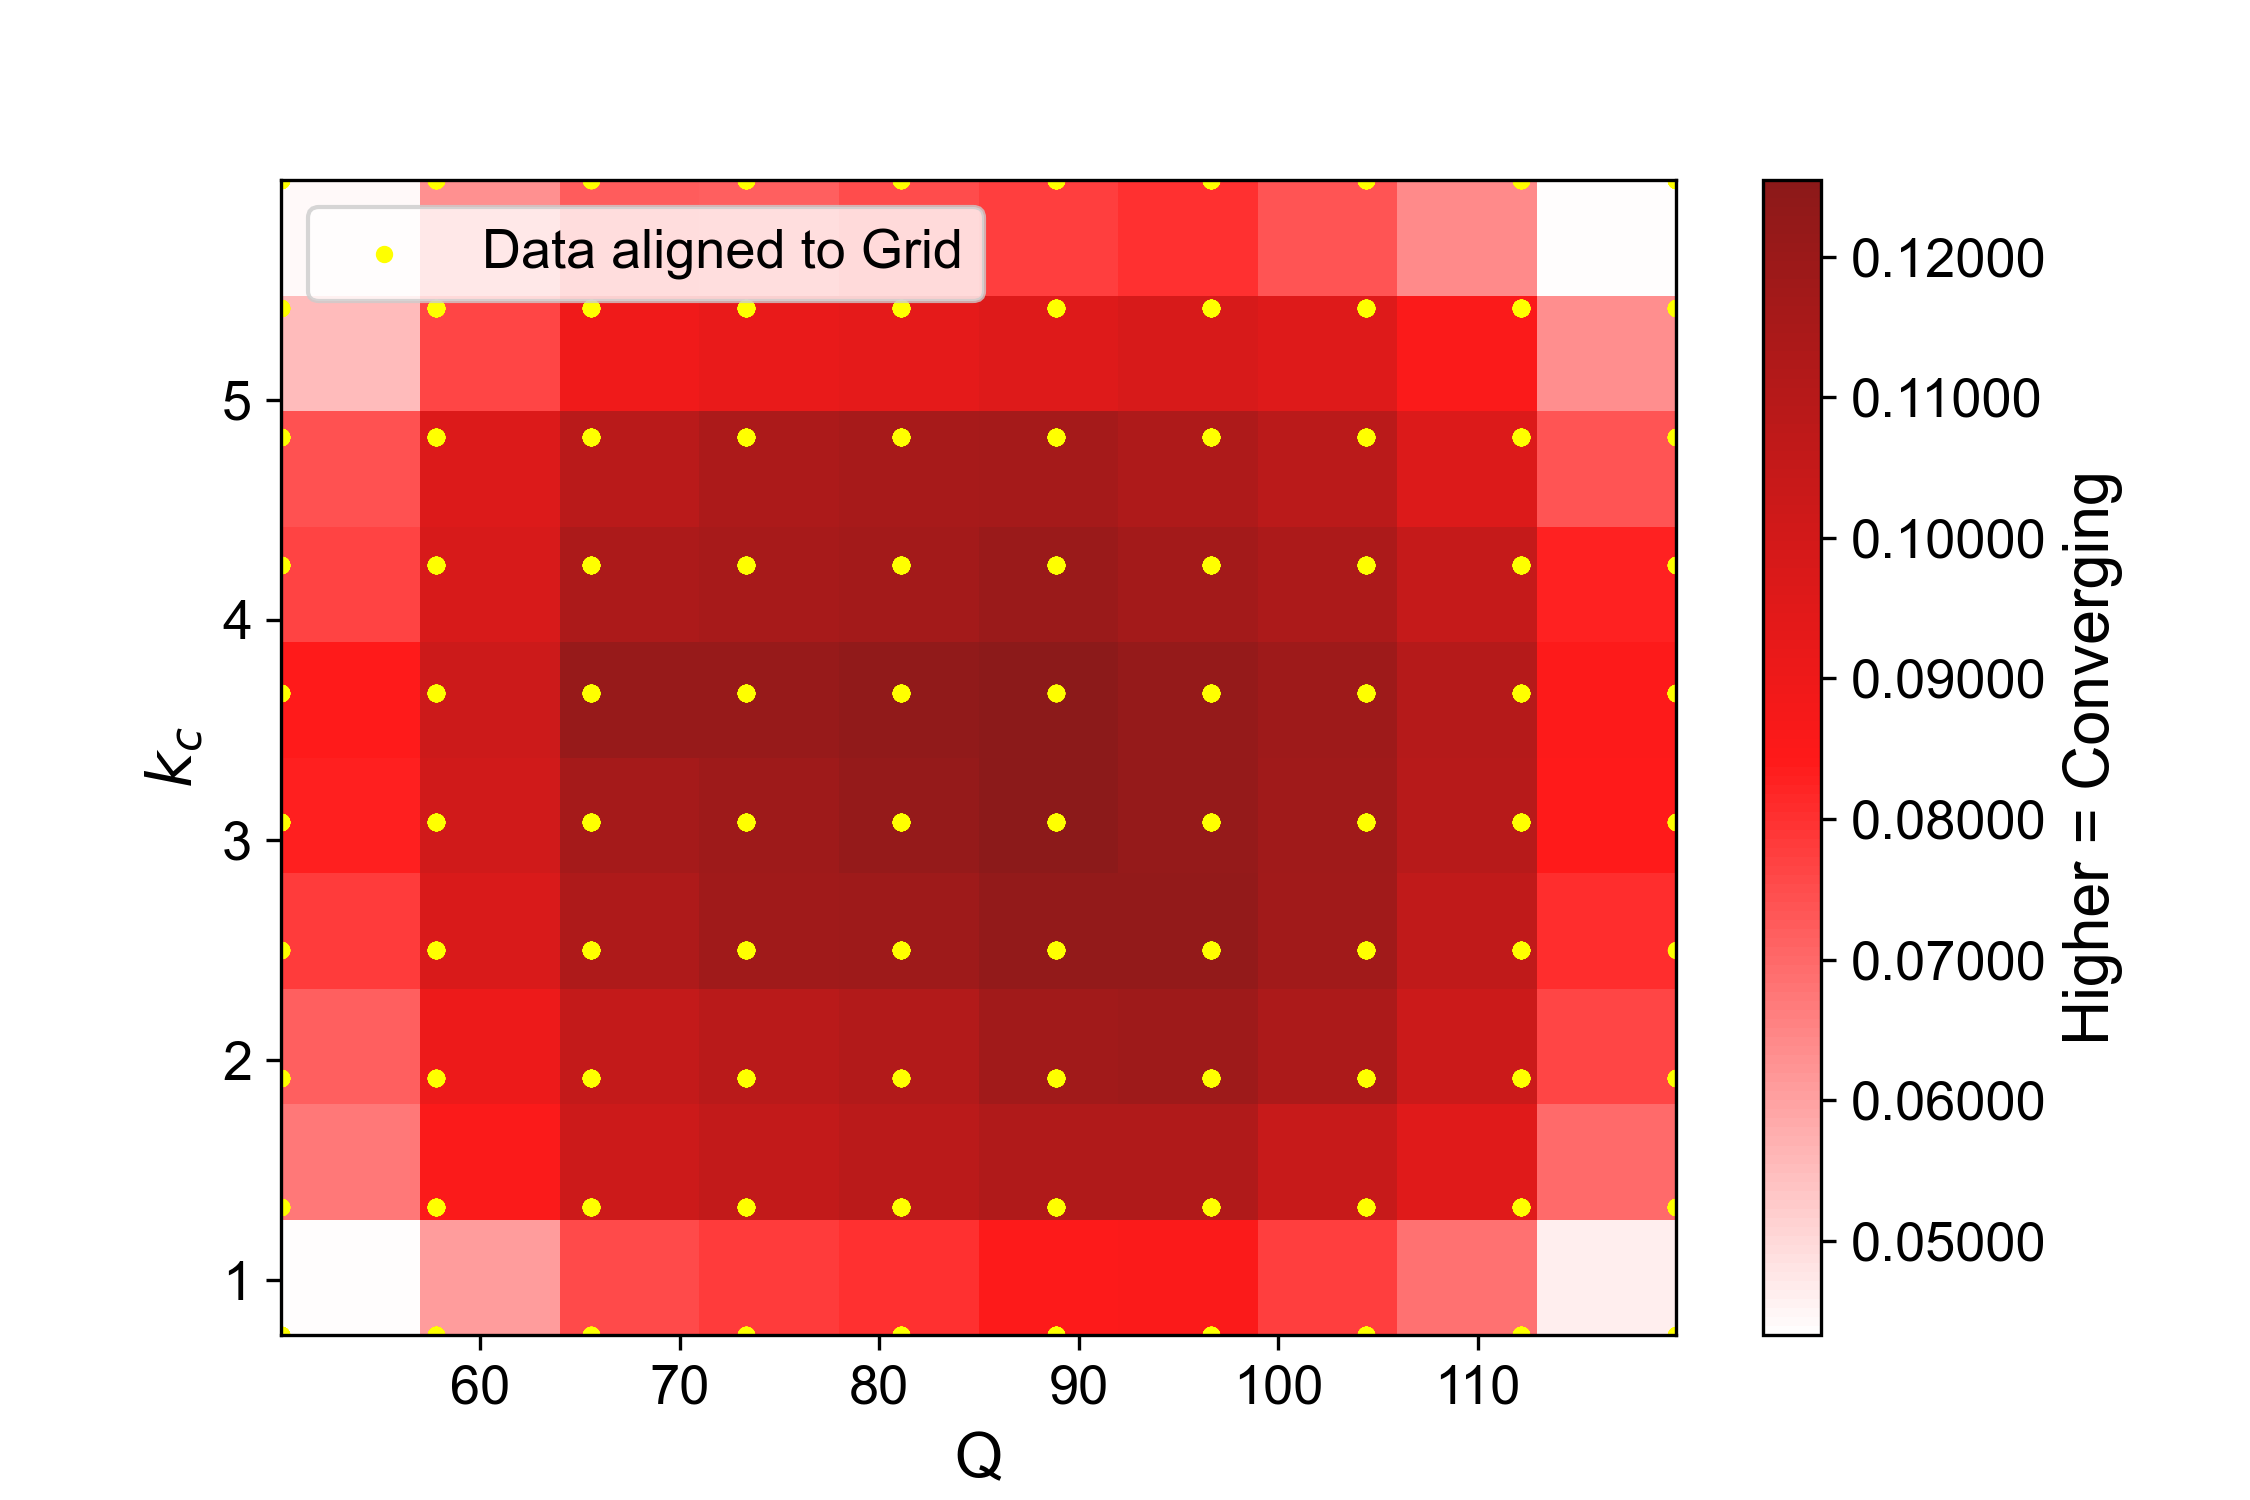
\includegraphics[width=0.32\textwidth]{figures/convergence/pairwise_projections_11.png} &
			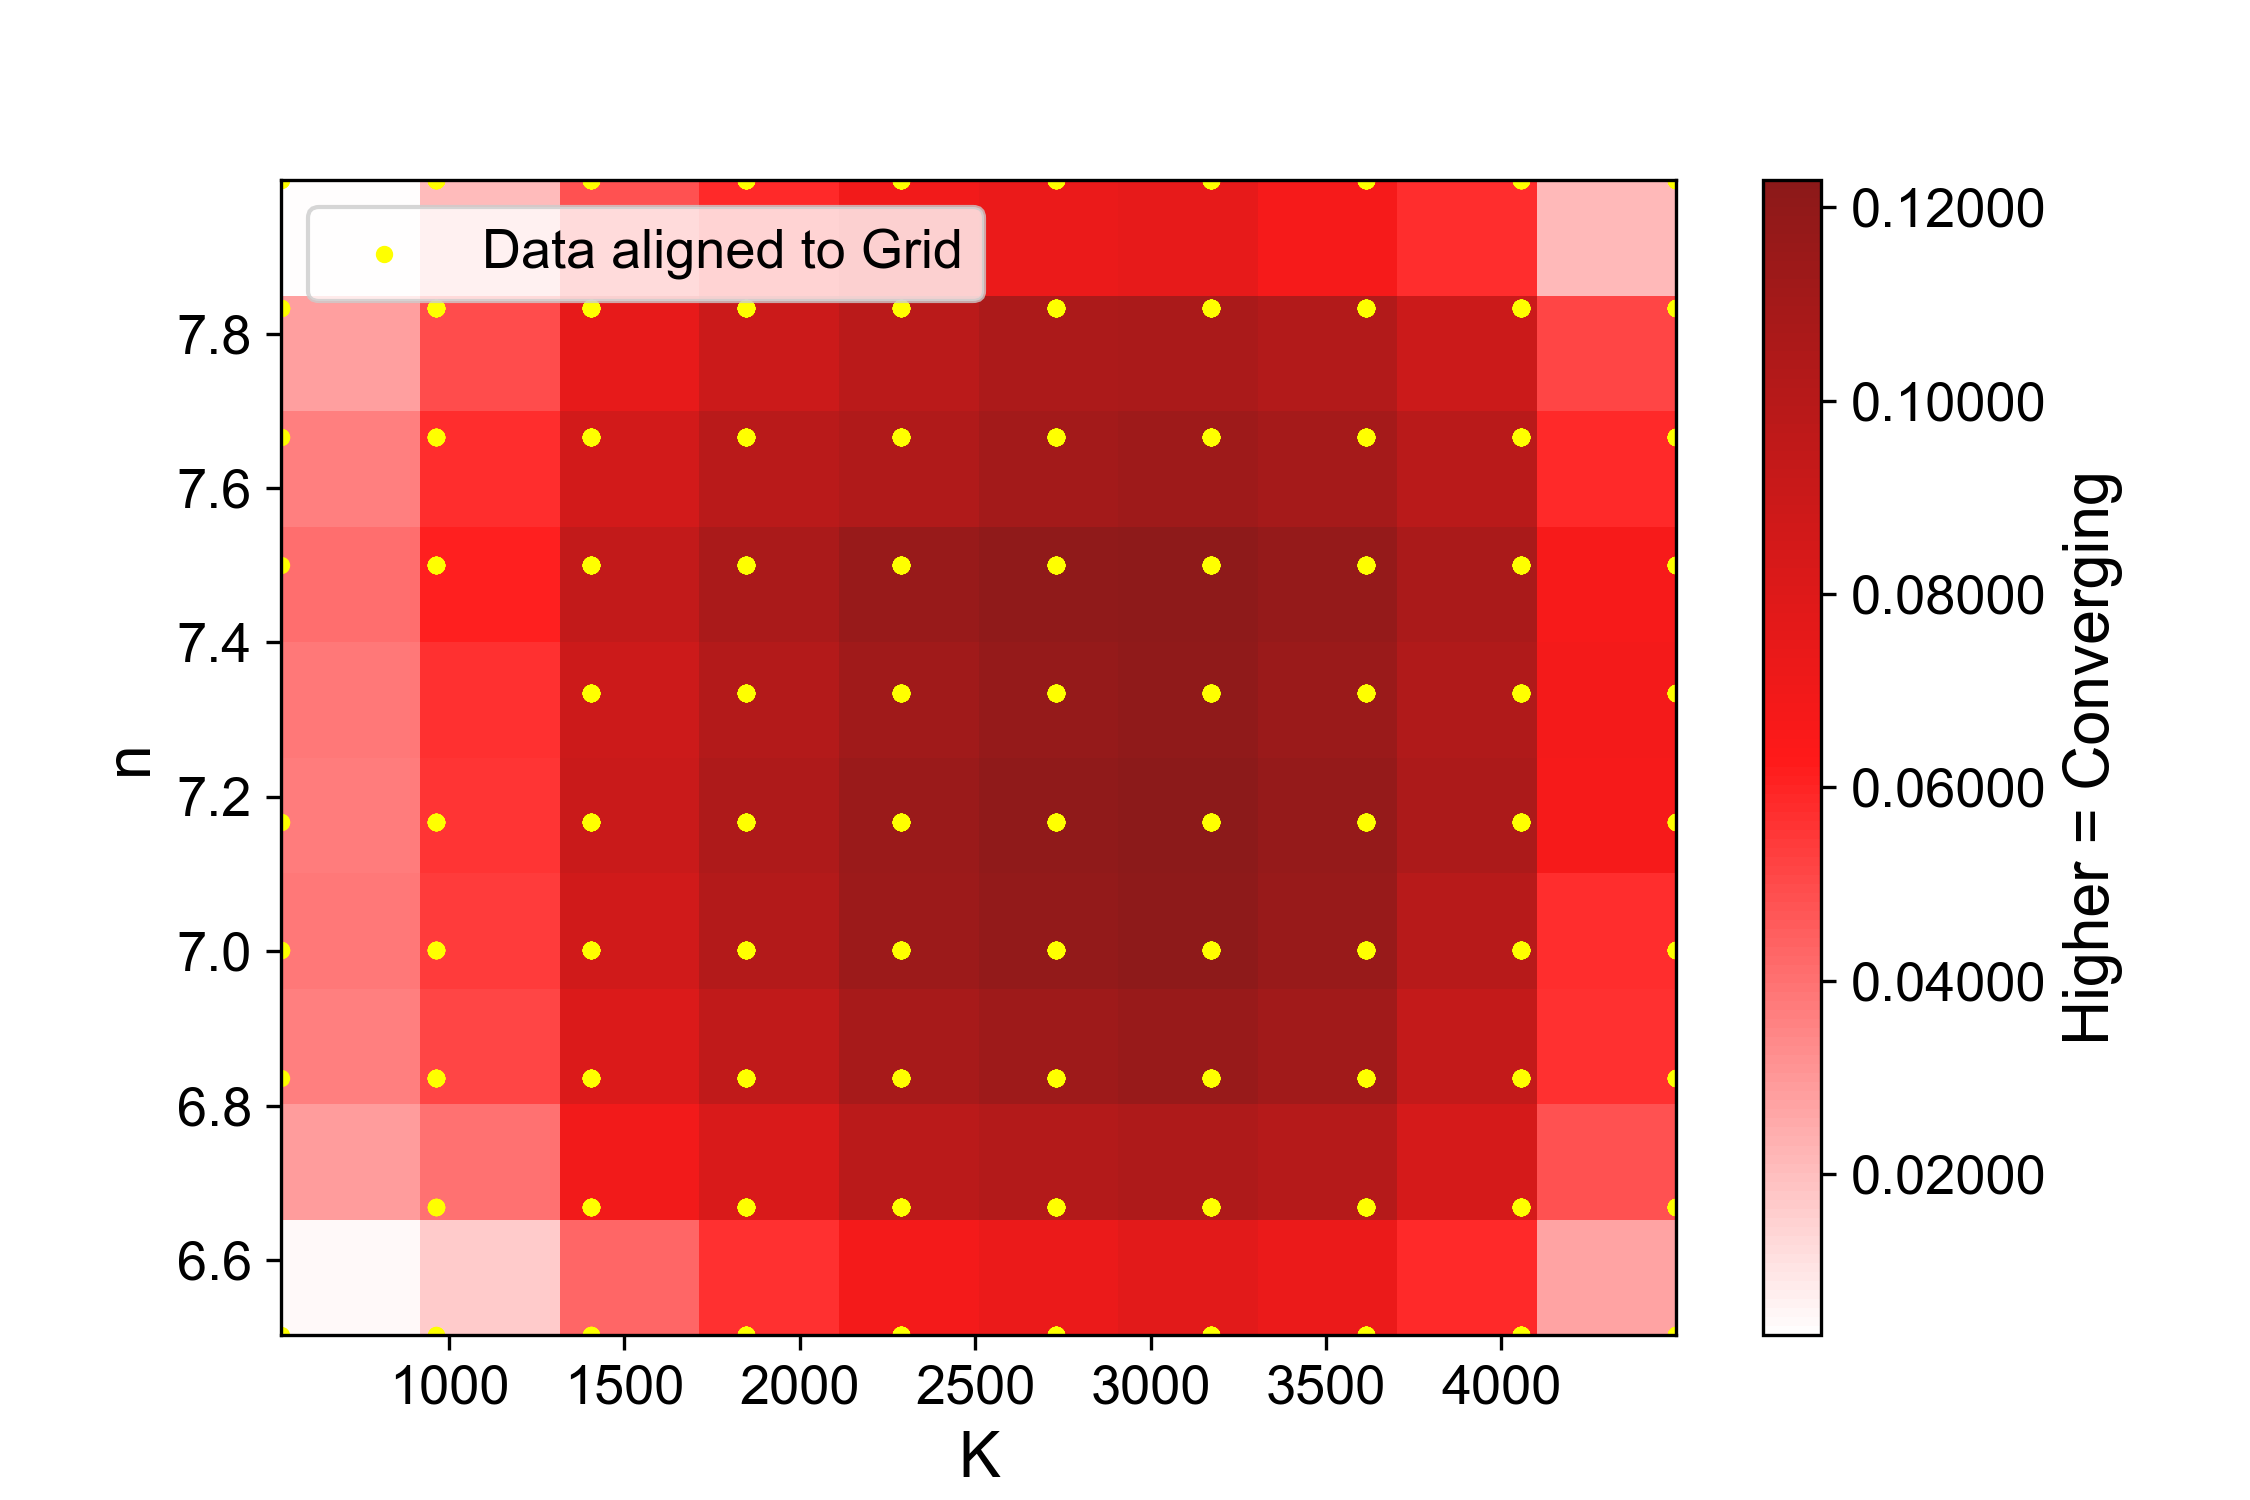
\includegraphics[width=0.32\textwidth]{figures/convergence/pairwise_projections_12.png} \\
			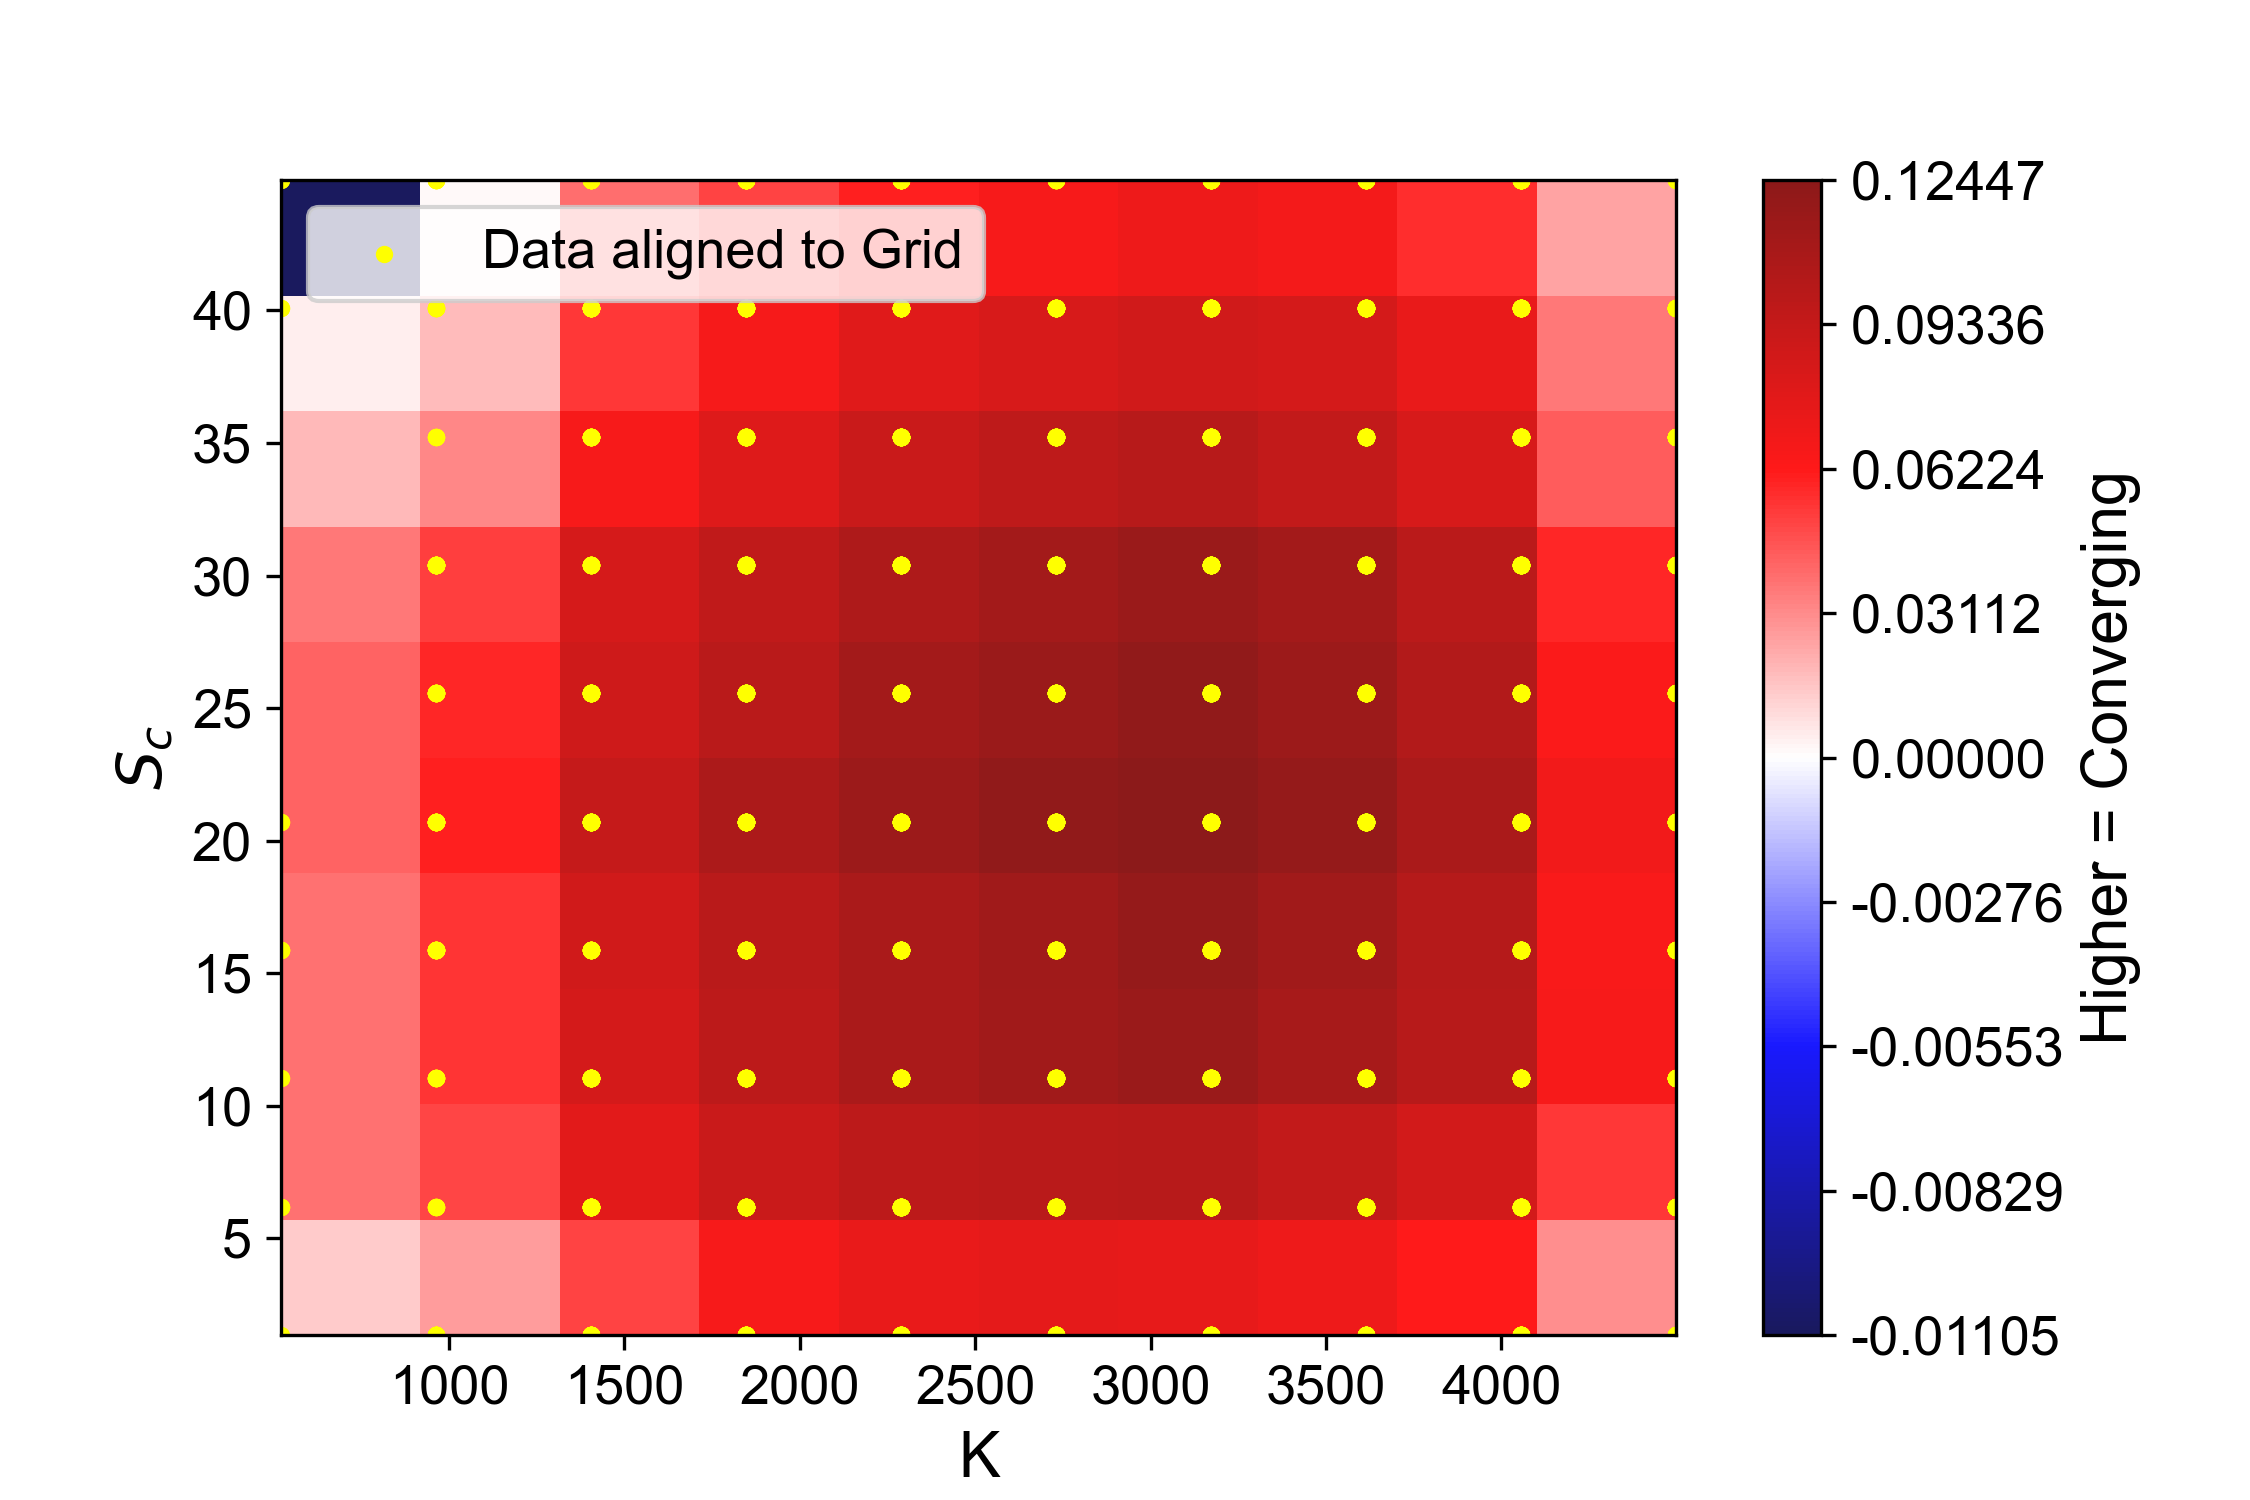
\includegraphics[width=0.32\textwidth]{figures/convergence/pairwise_projections_13.png} &
			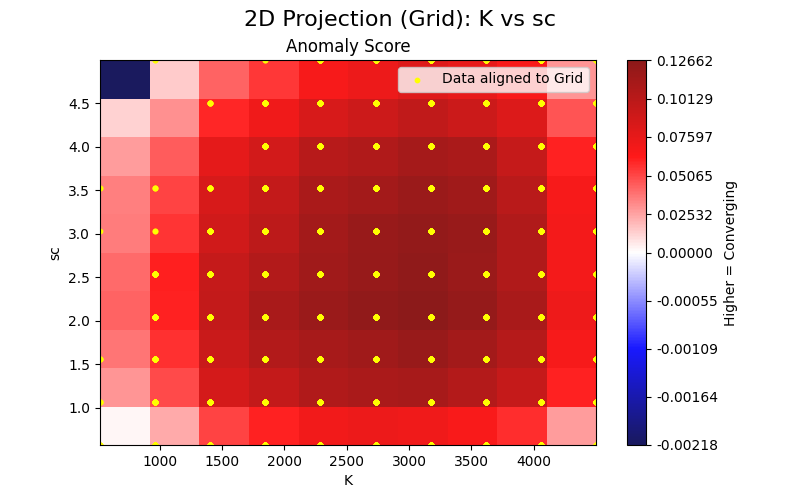
\includegraphics[width=0.32\textwidth]{figures/convergence/pairwise_projections_14.png} &
			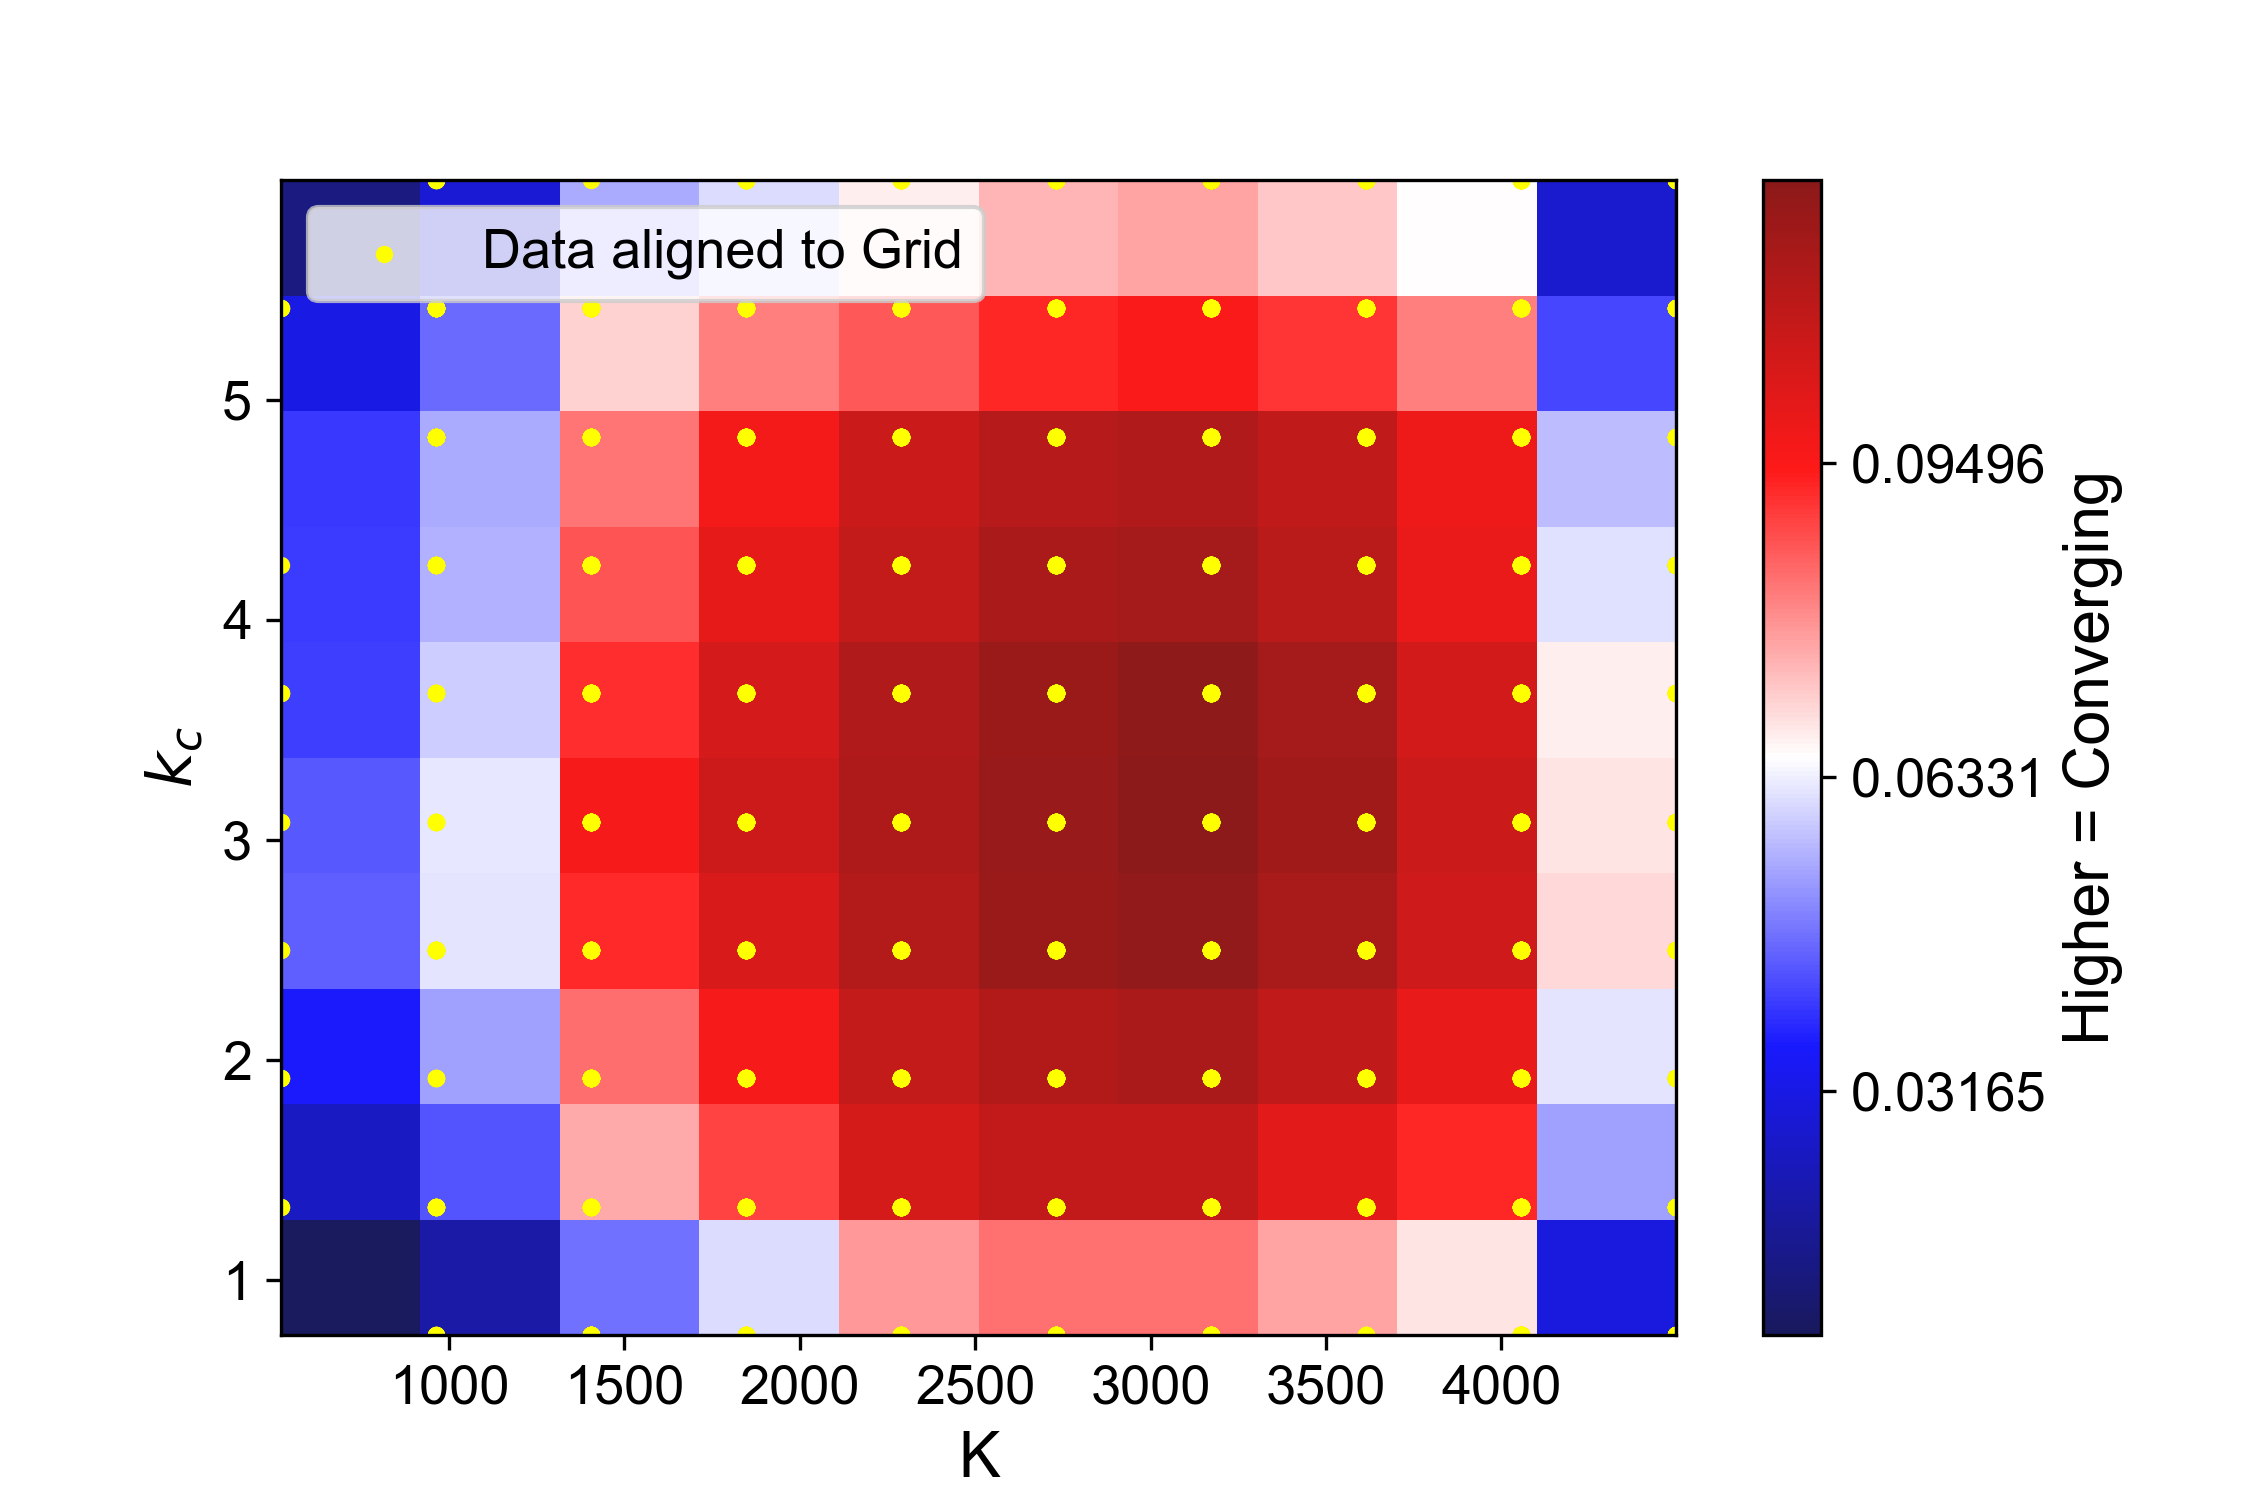
\includegraphics[width=0.32\textwidth]{figures/convergence/pairwise_projections_15.png} \\
			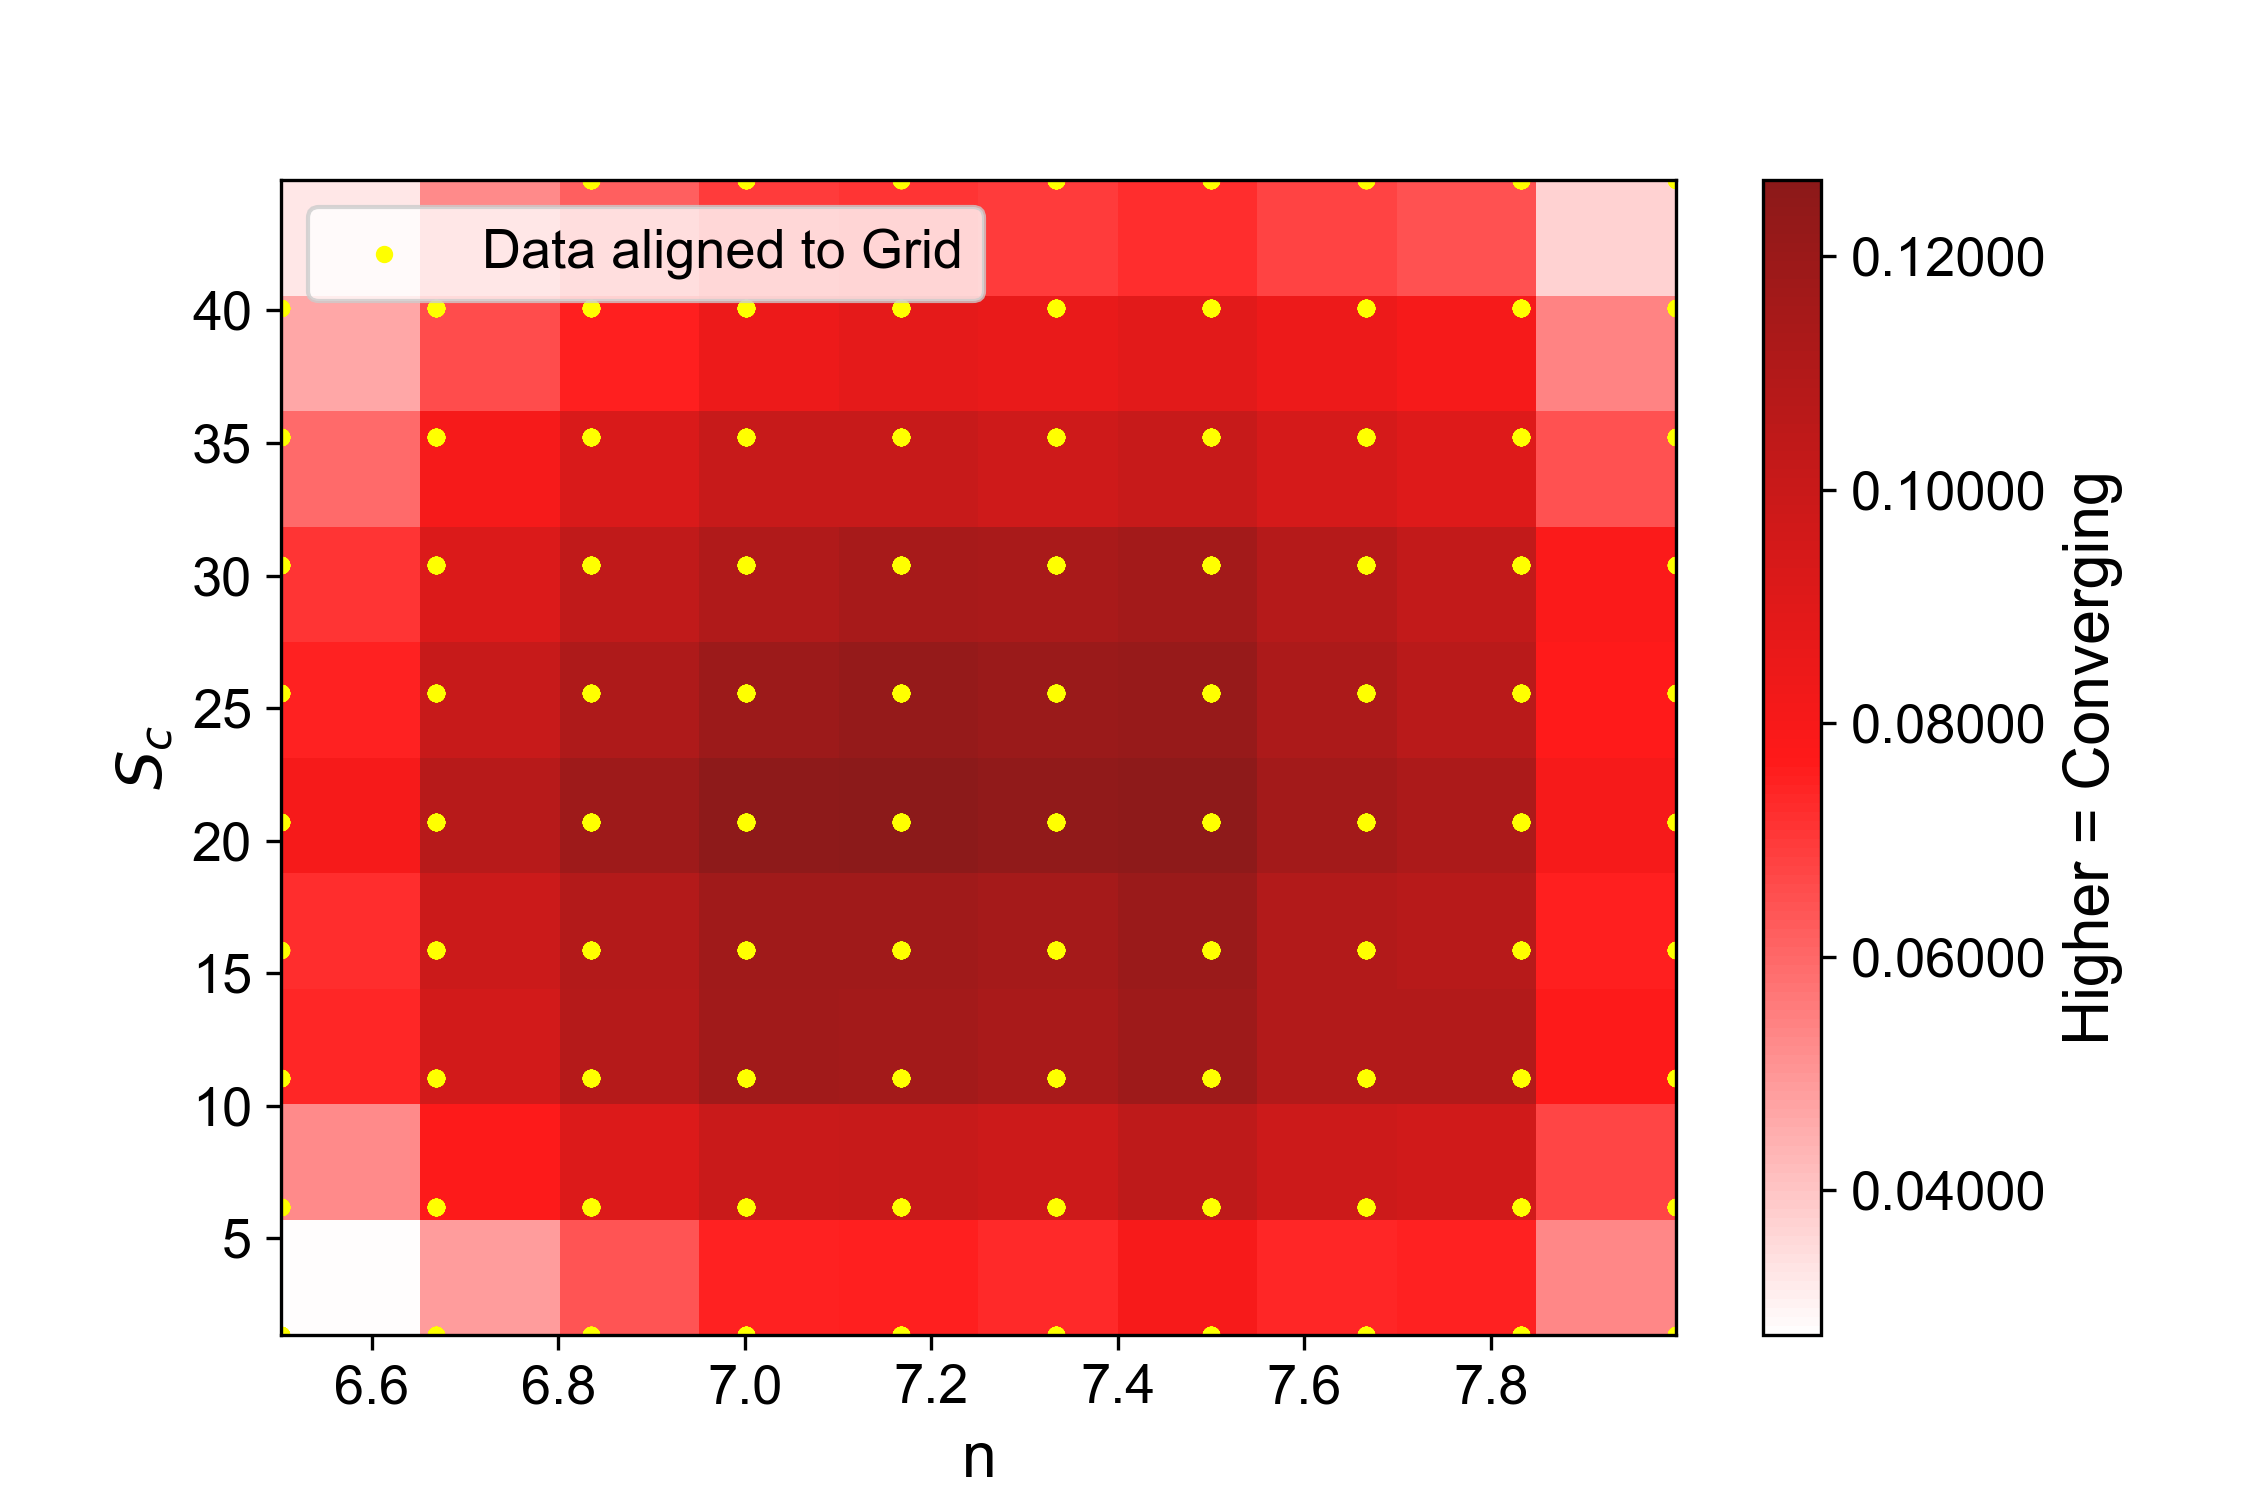
\includegraphics[width=0.32\textwidth]{figures/convergence/pairwise_projections_16.png} &
			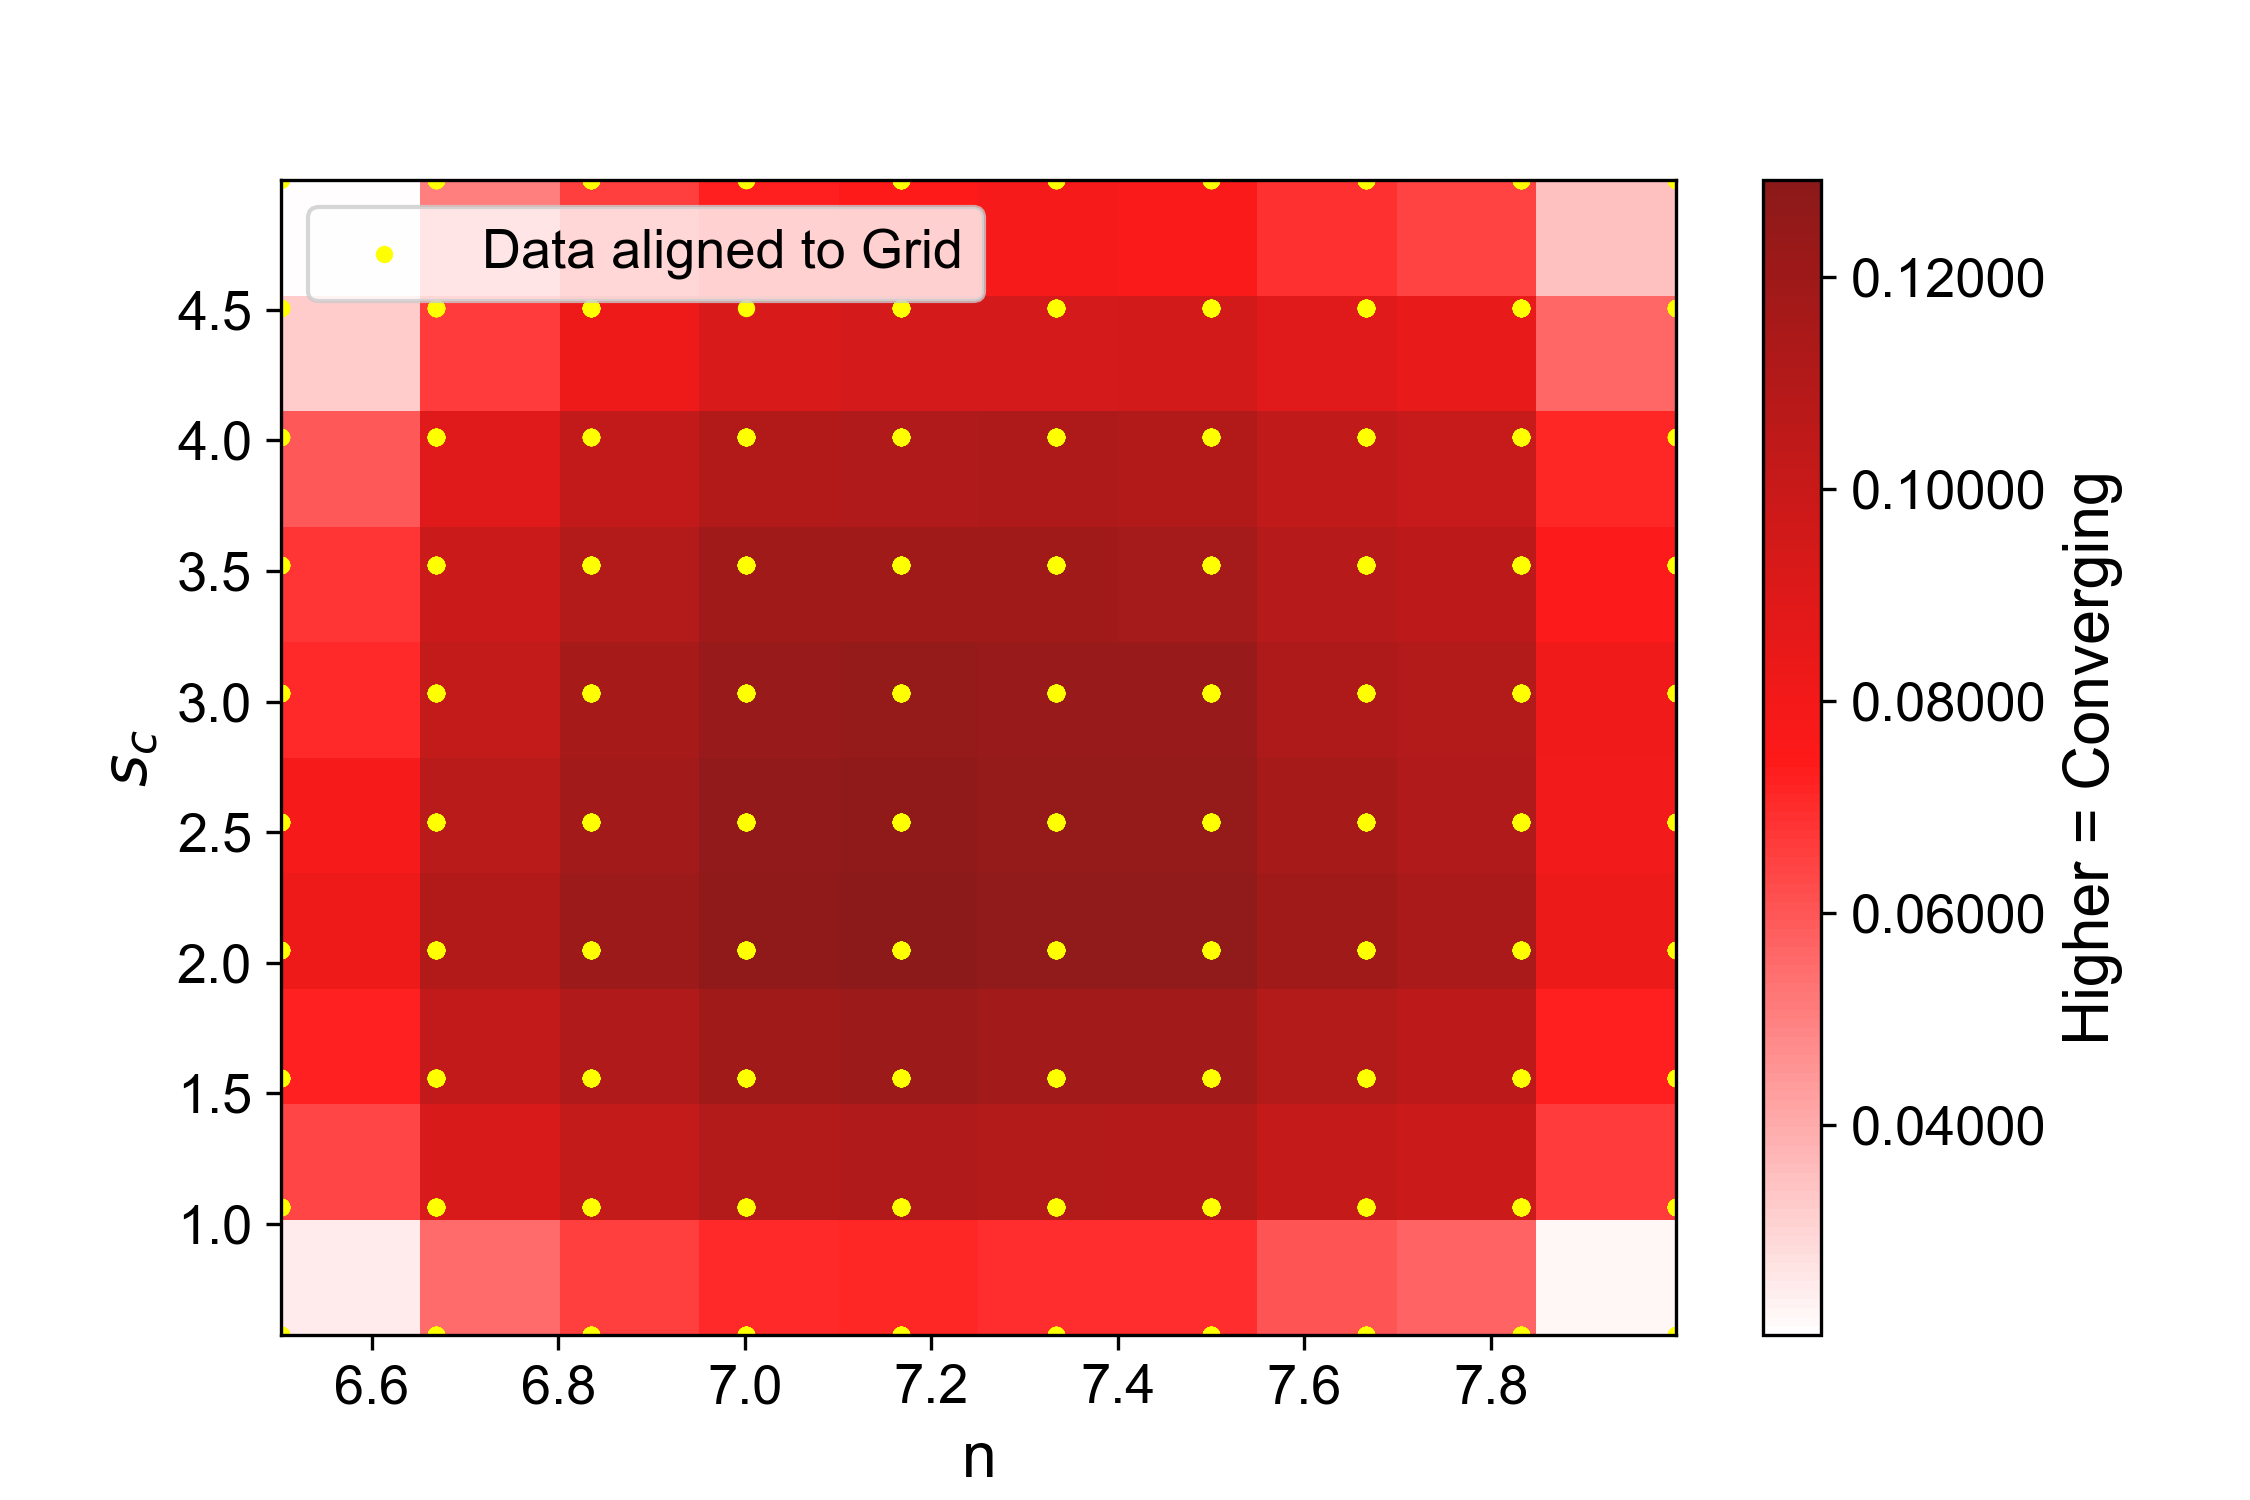
\includegraphics[width=0.32\textwidth]{figures/convergence/pairwise_projections_17.png} &
			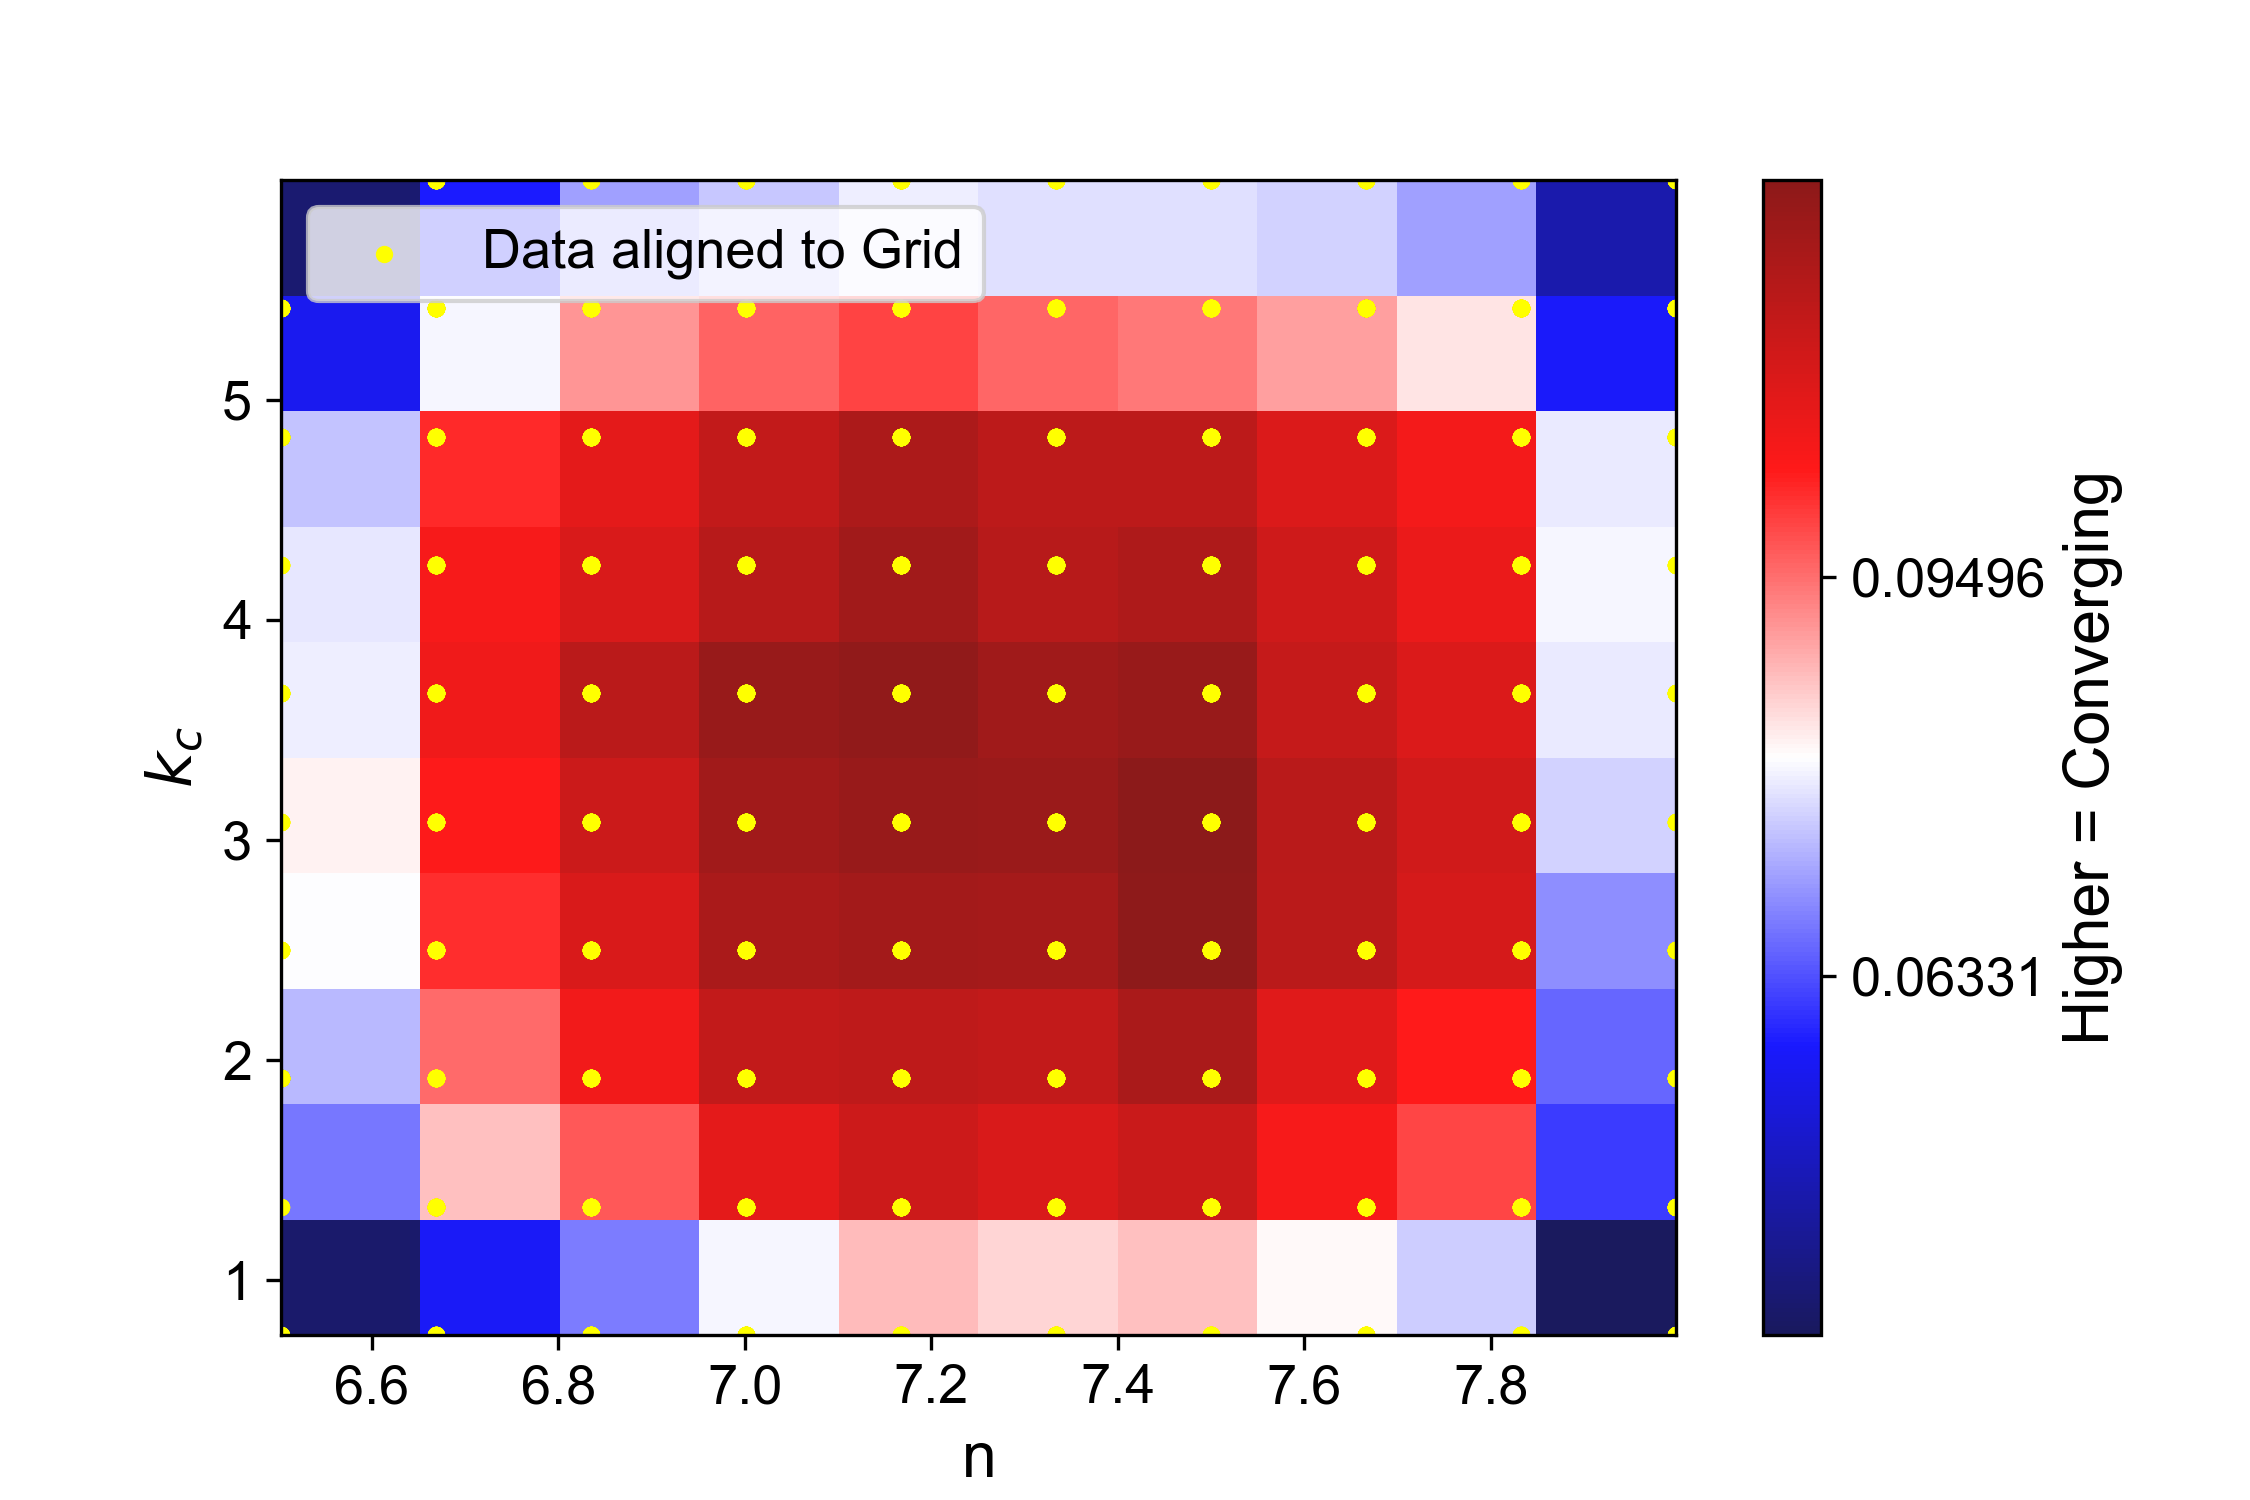
\includegraphics[width=0.32\textwidth]{figures/convergence/pairwise_projections_18.png} \\
			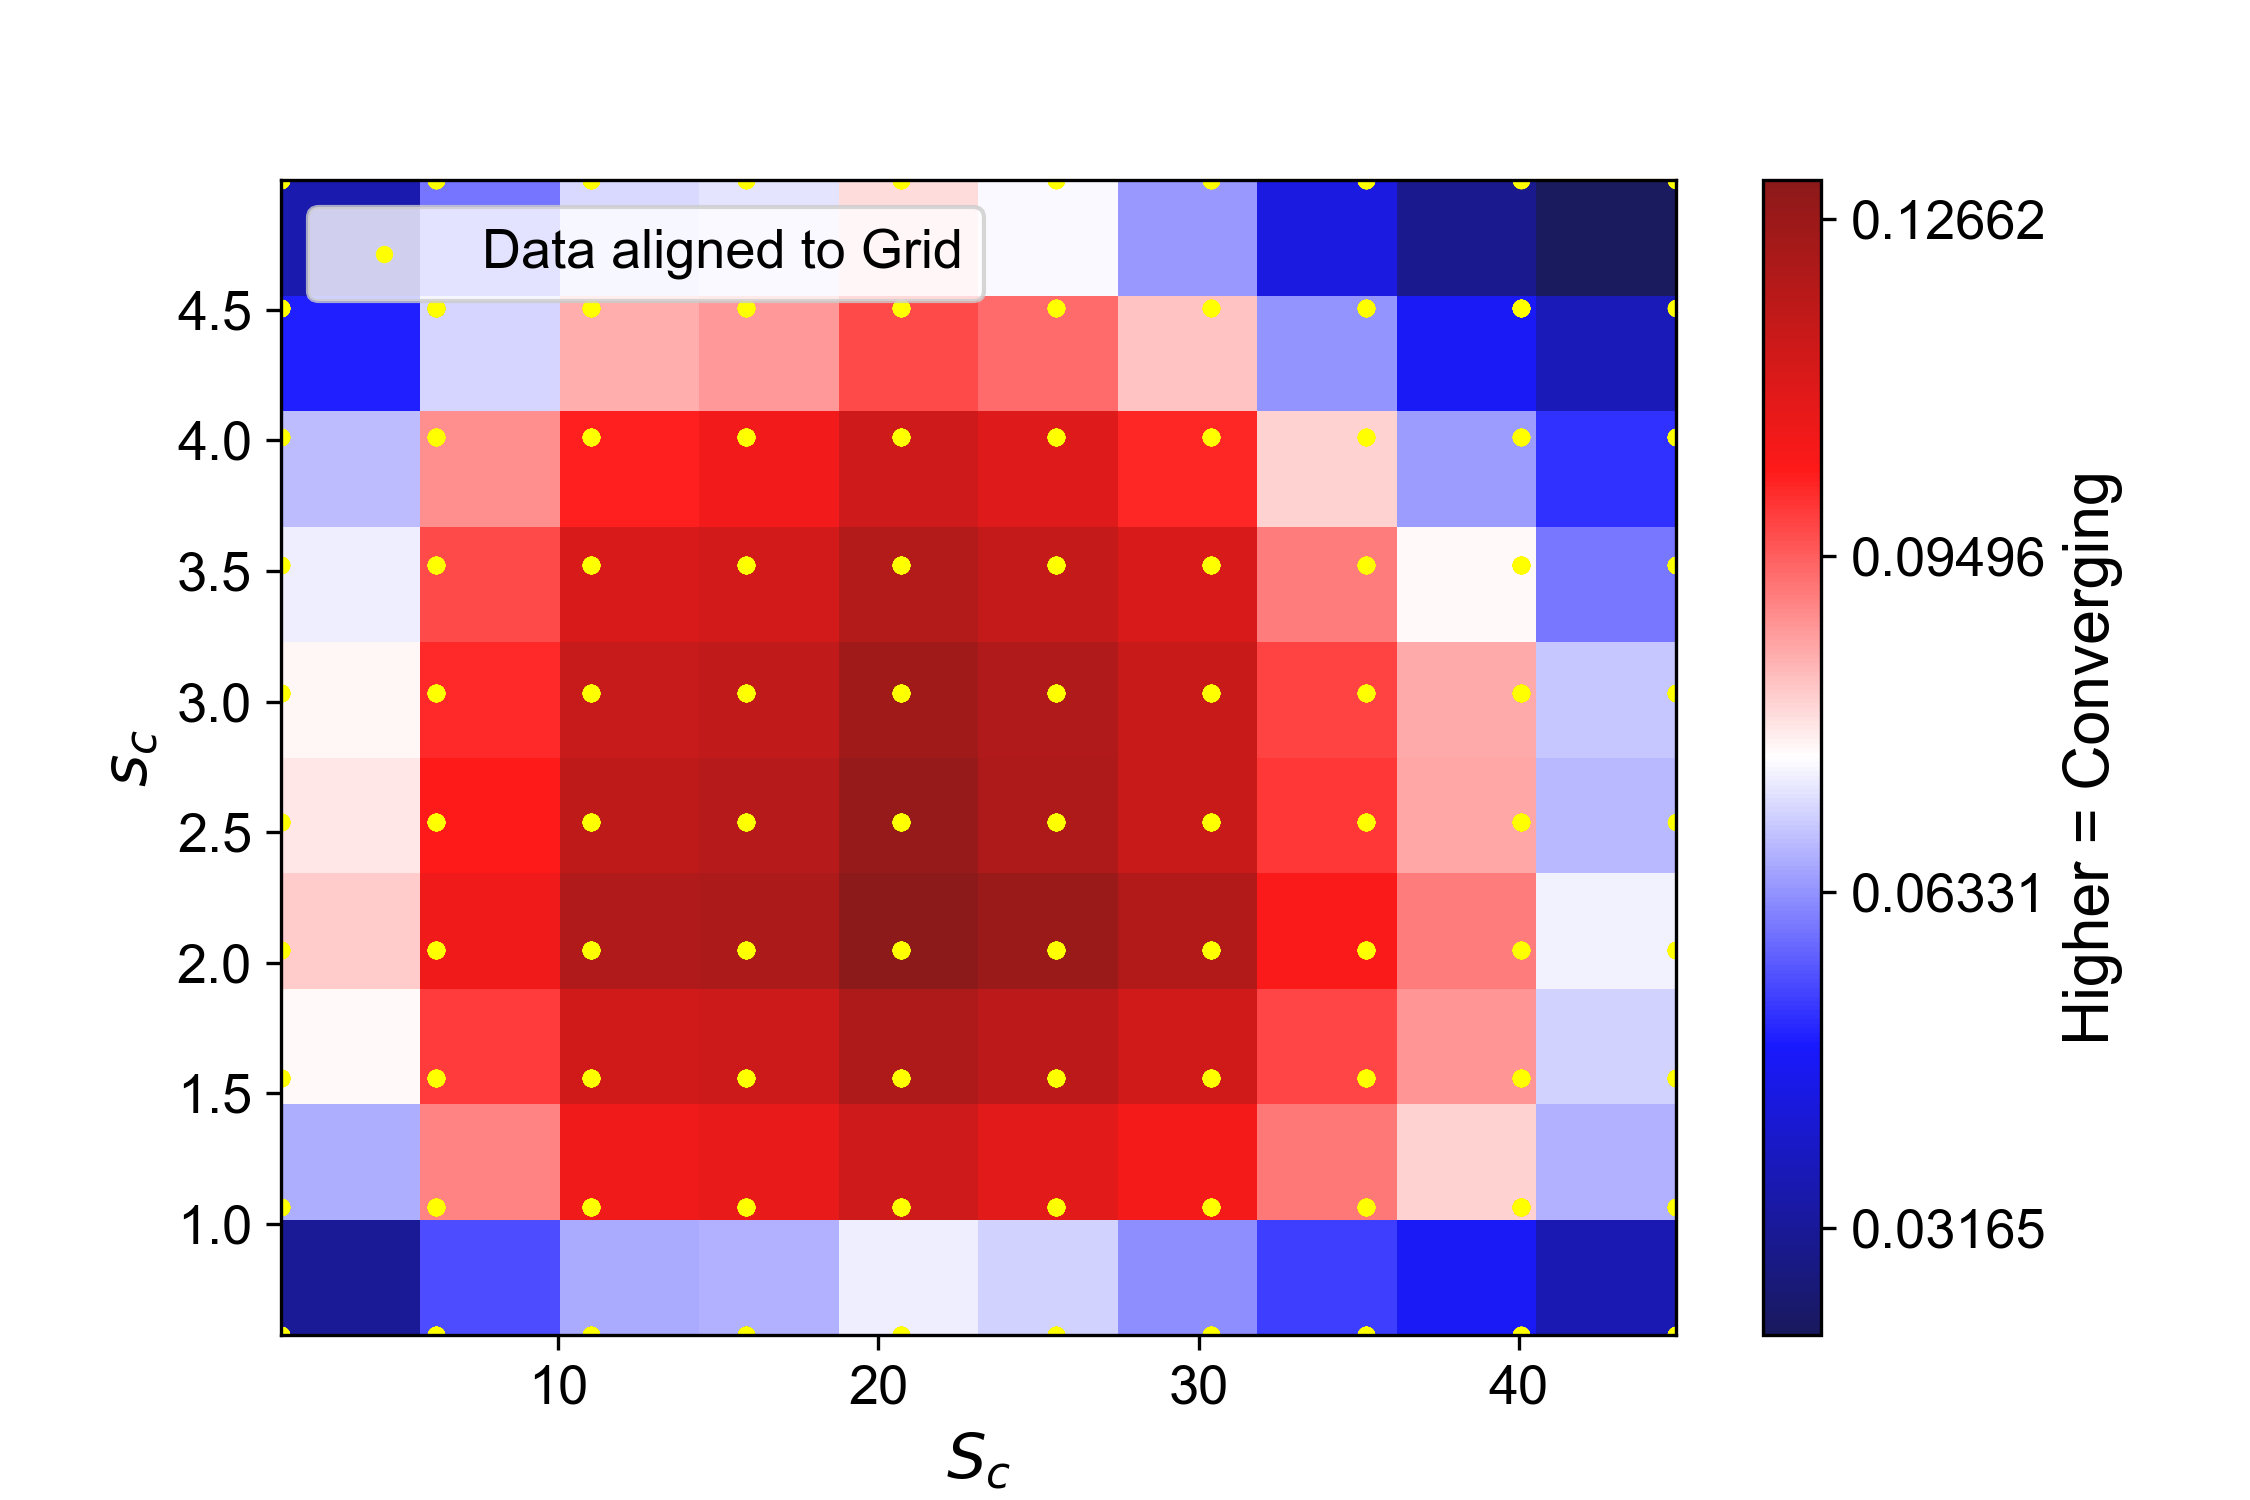
\includegraphics[width=0.32\textwidth]{figures/convergence/pairwise_projections_19.png} &
			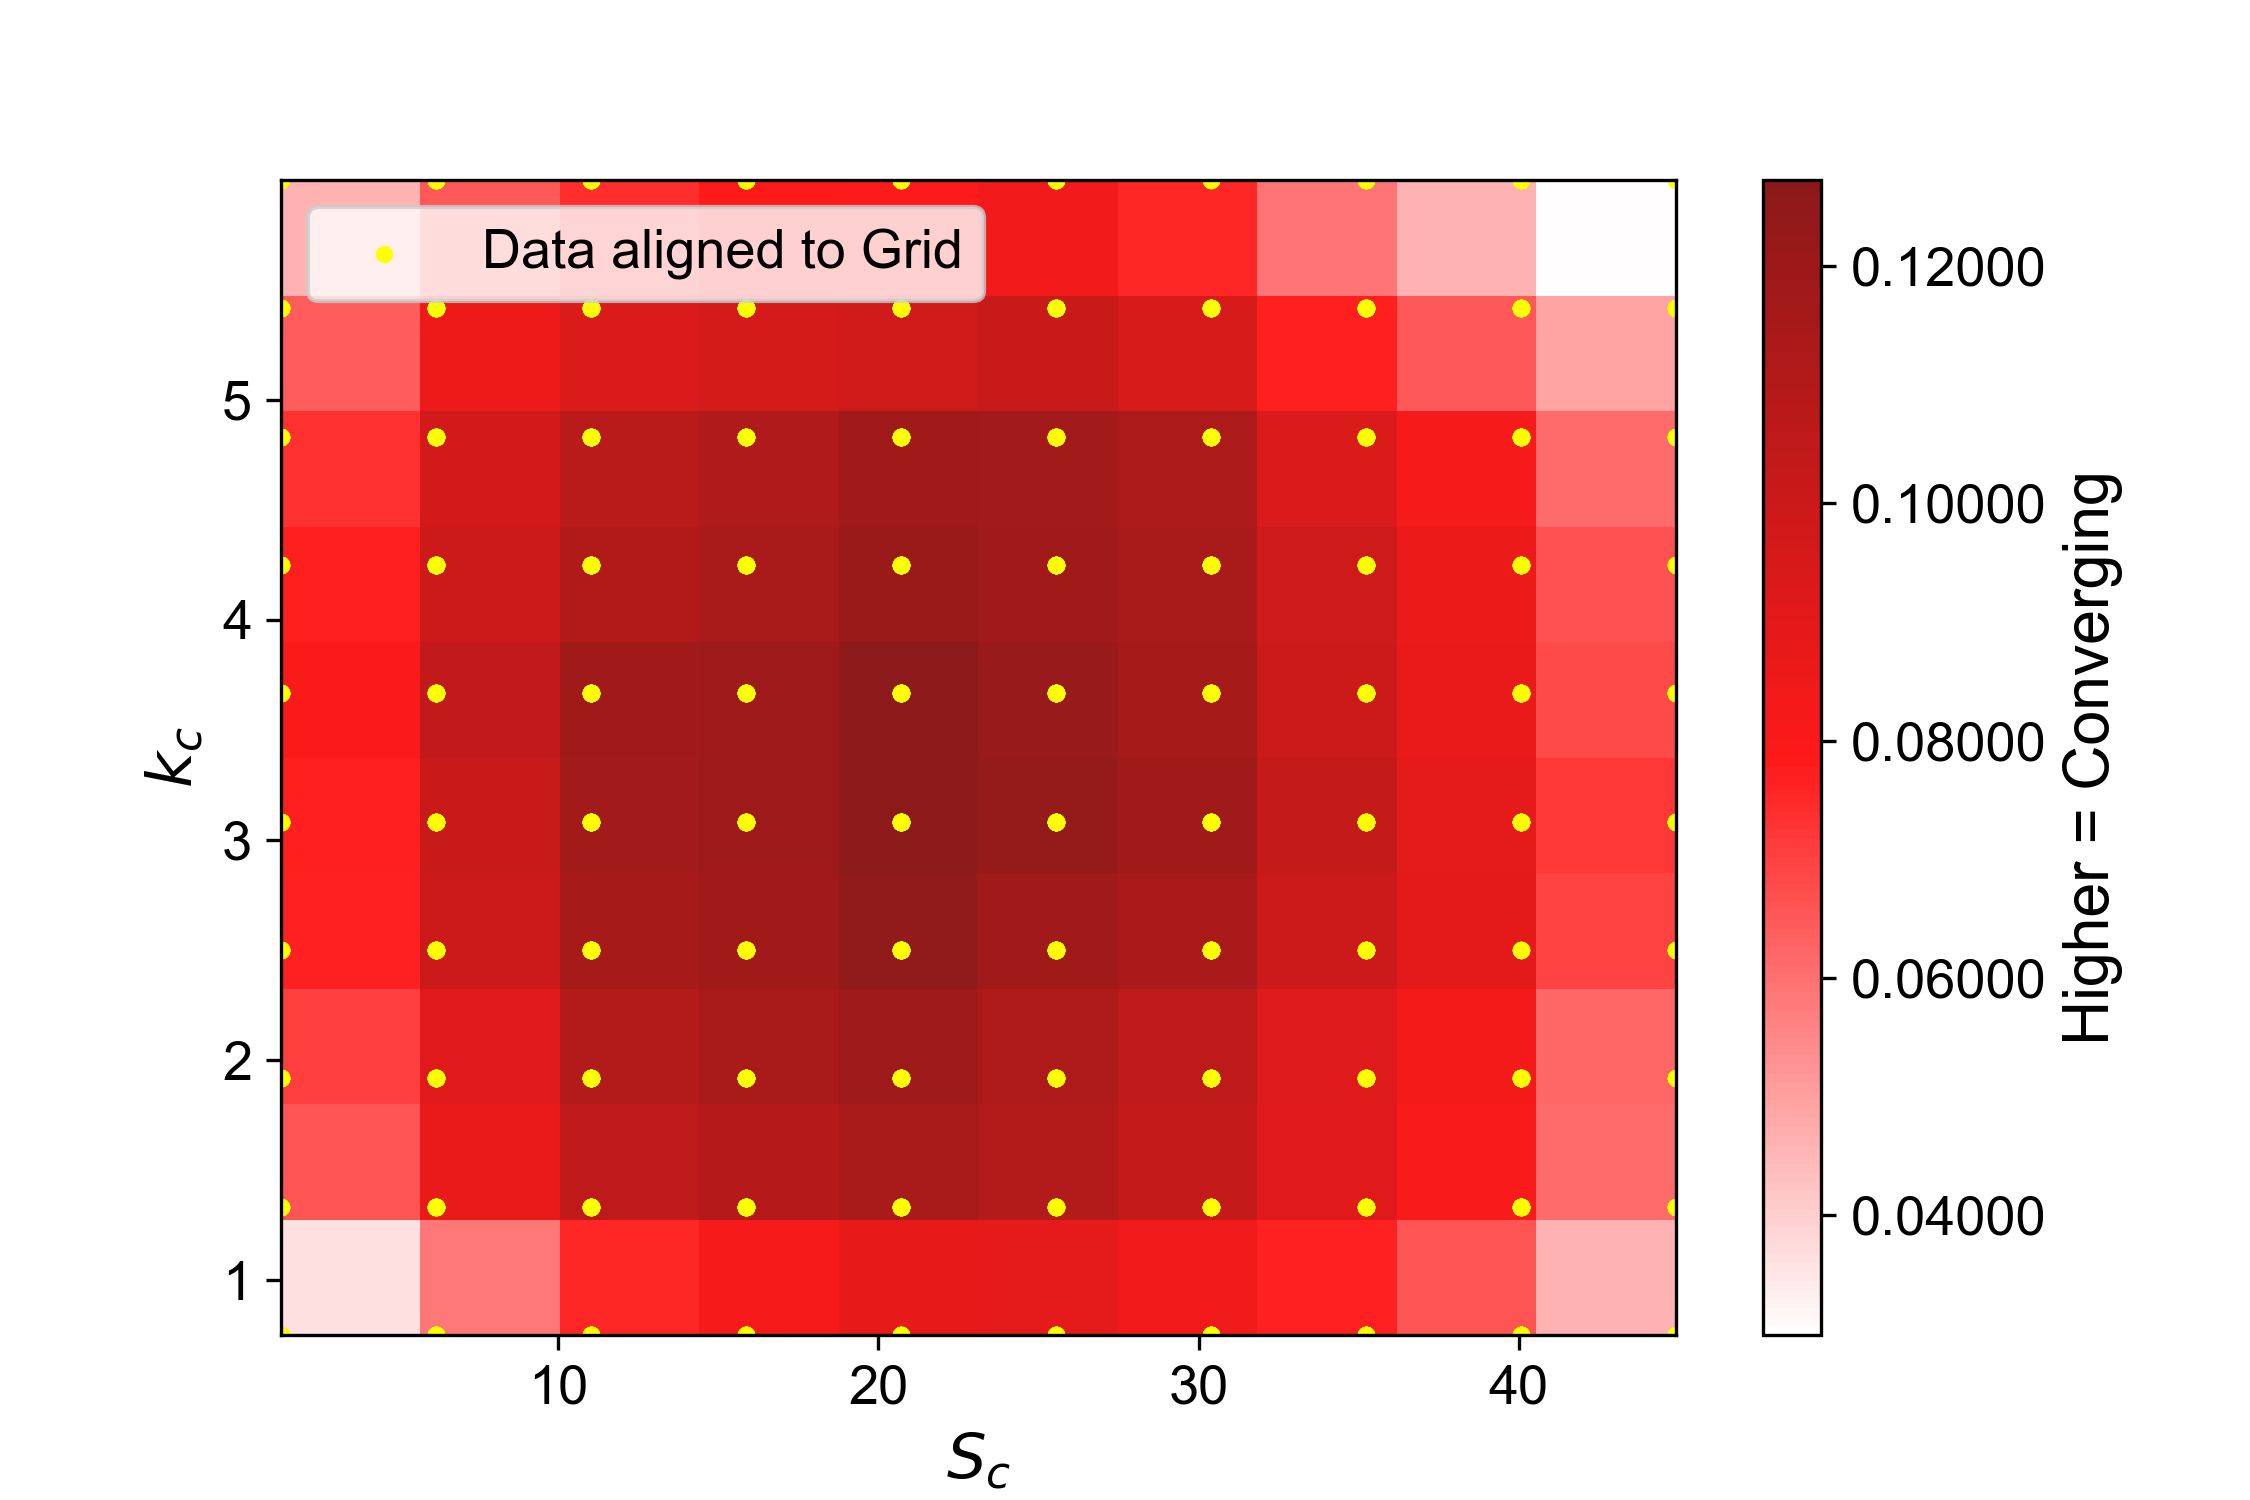
\includegraphics[width=0.32\textwidth]{figures/convergence/pairwise_projections_20.png} &
			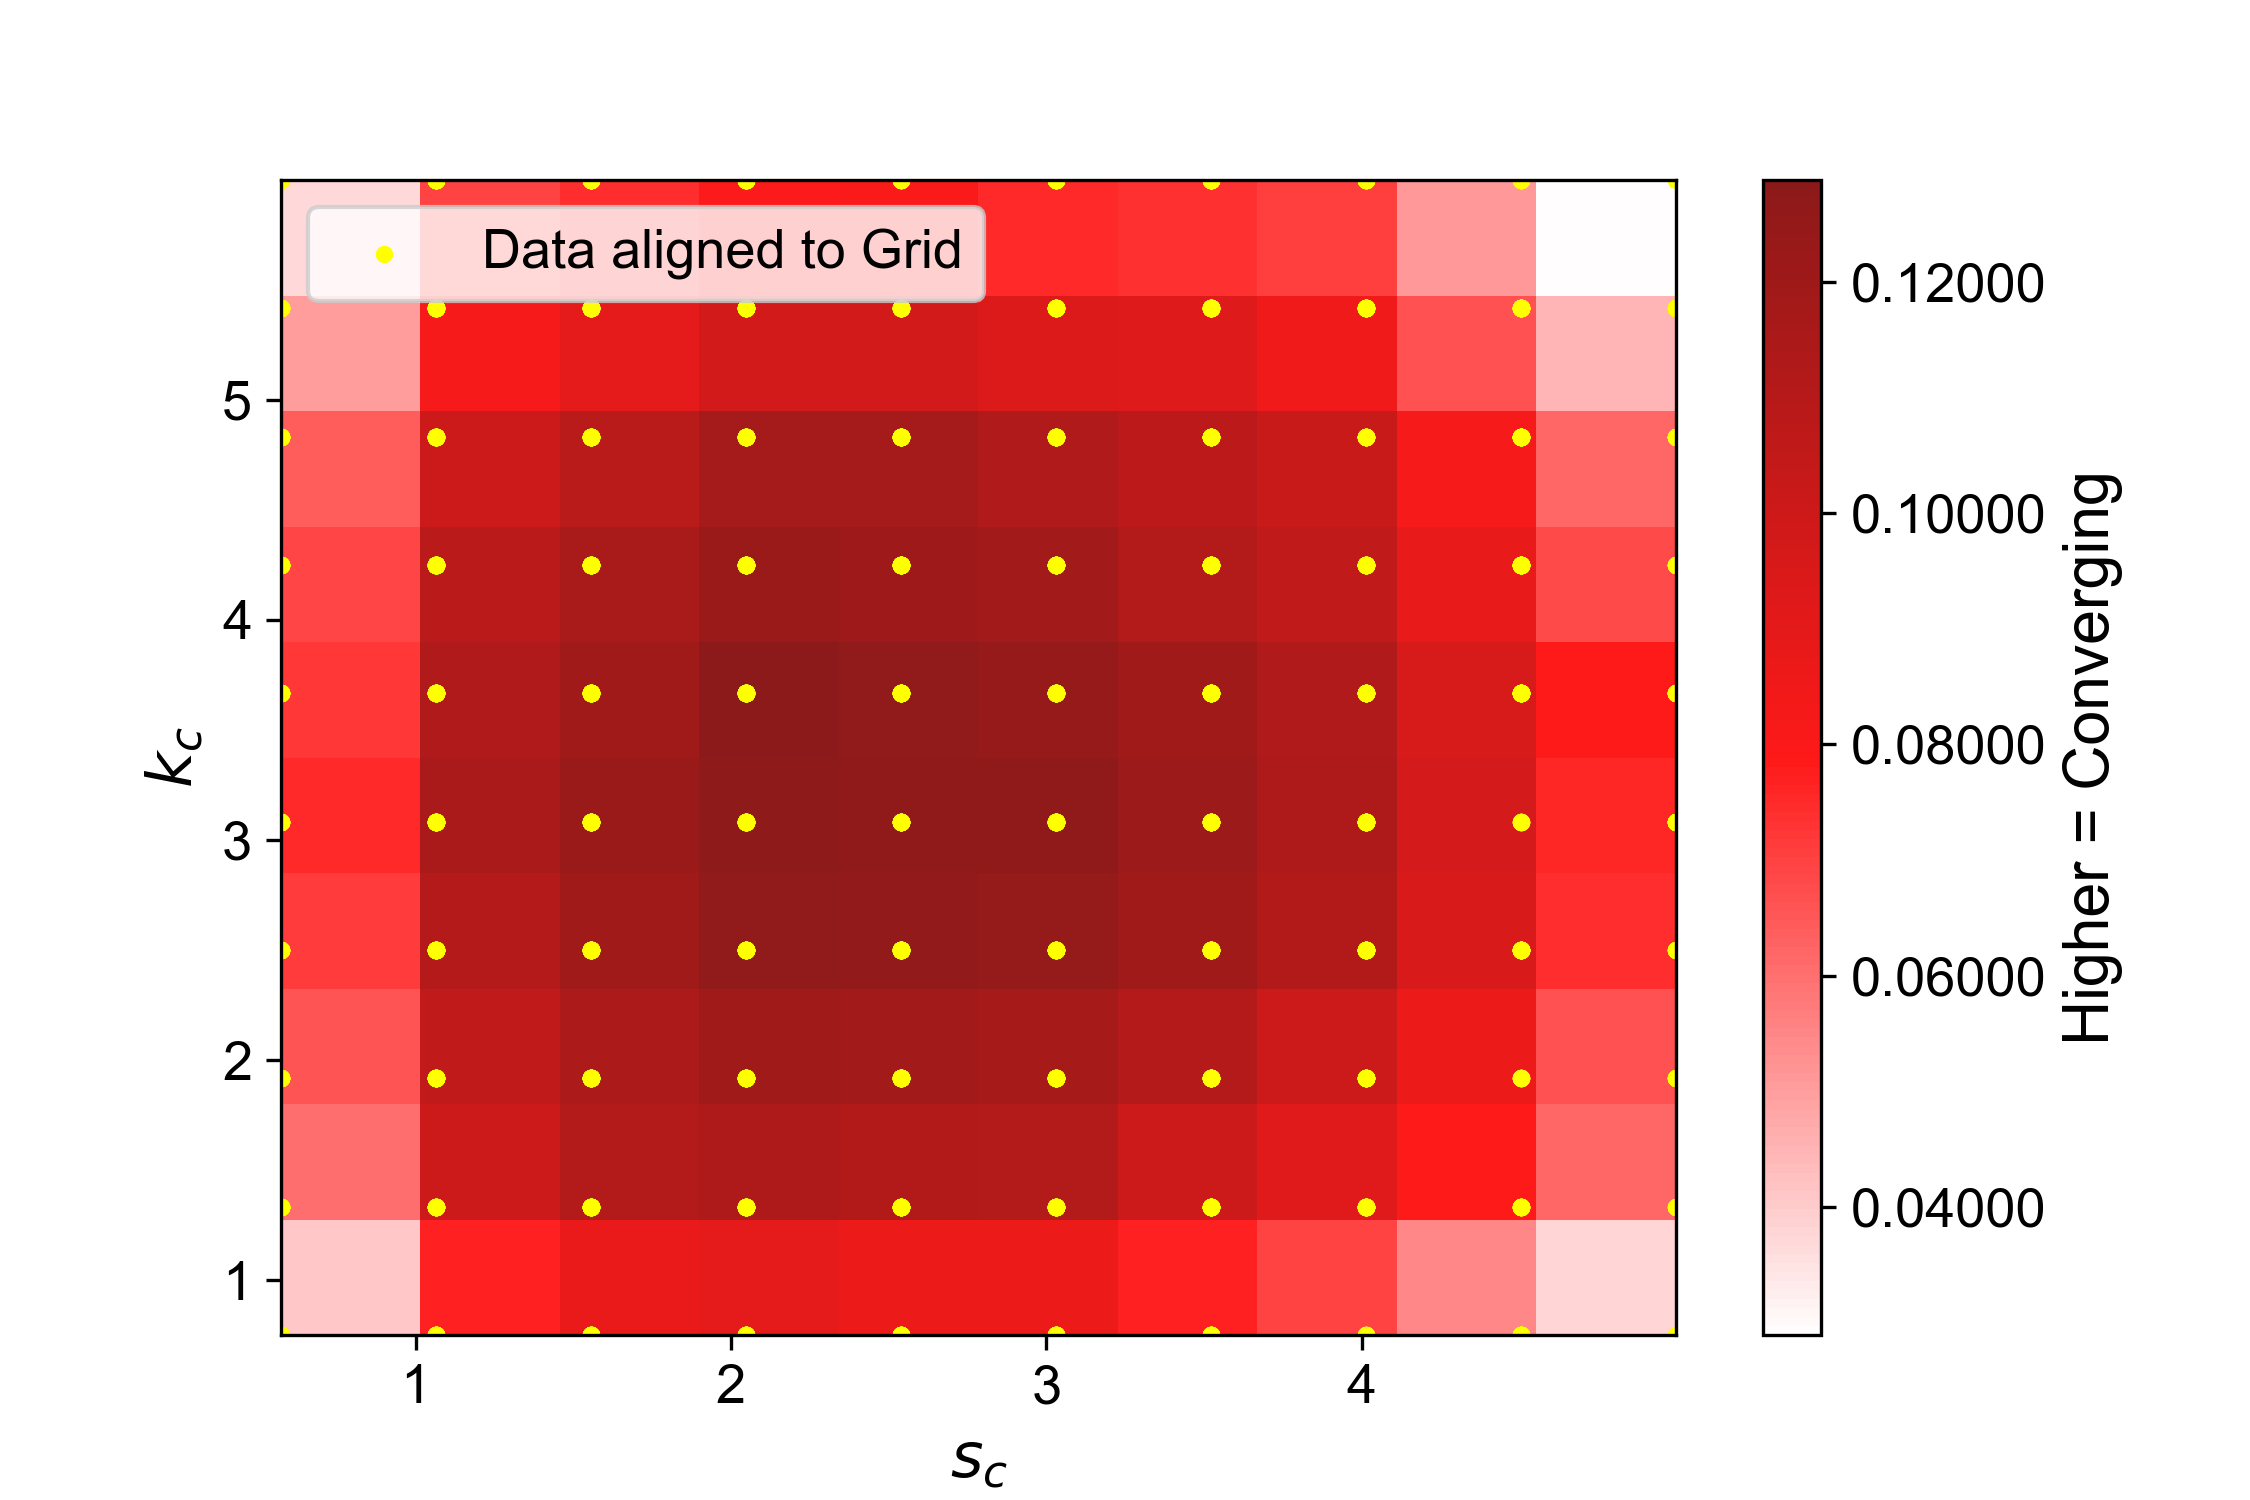
\includegraphics[width=0.32\textwidth]{figures/convergence/pairwise_projections_21.png} 
			% Continue until 21 images
		\end{tabular}
		\caption{Pairwise projections of the material model parameters.}
		\label{fig:pairwise_projections}
	\end{figure}
	
	\noindent
	\begin{minipage}{\textwidth}
		The creep curves sampled from the active learning are shown in the figure~\ref{fig:creep_curves_AL_lagamine}. Only 980 curves converged when the model parameters were input to Lagamine solver.
		
		\vspace{1em}
		\begin{center}
			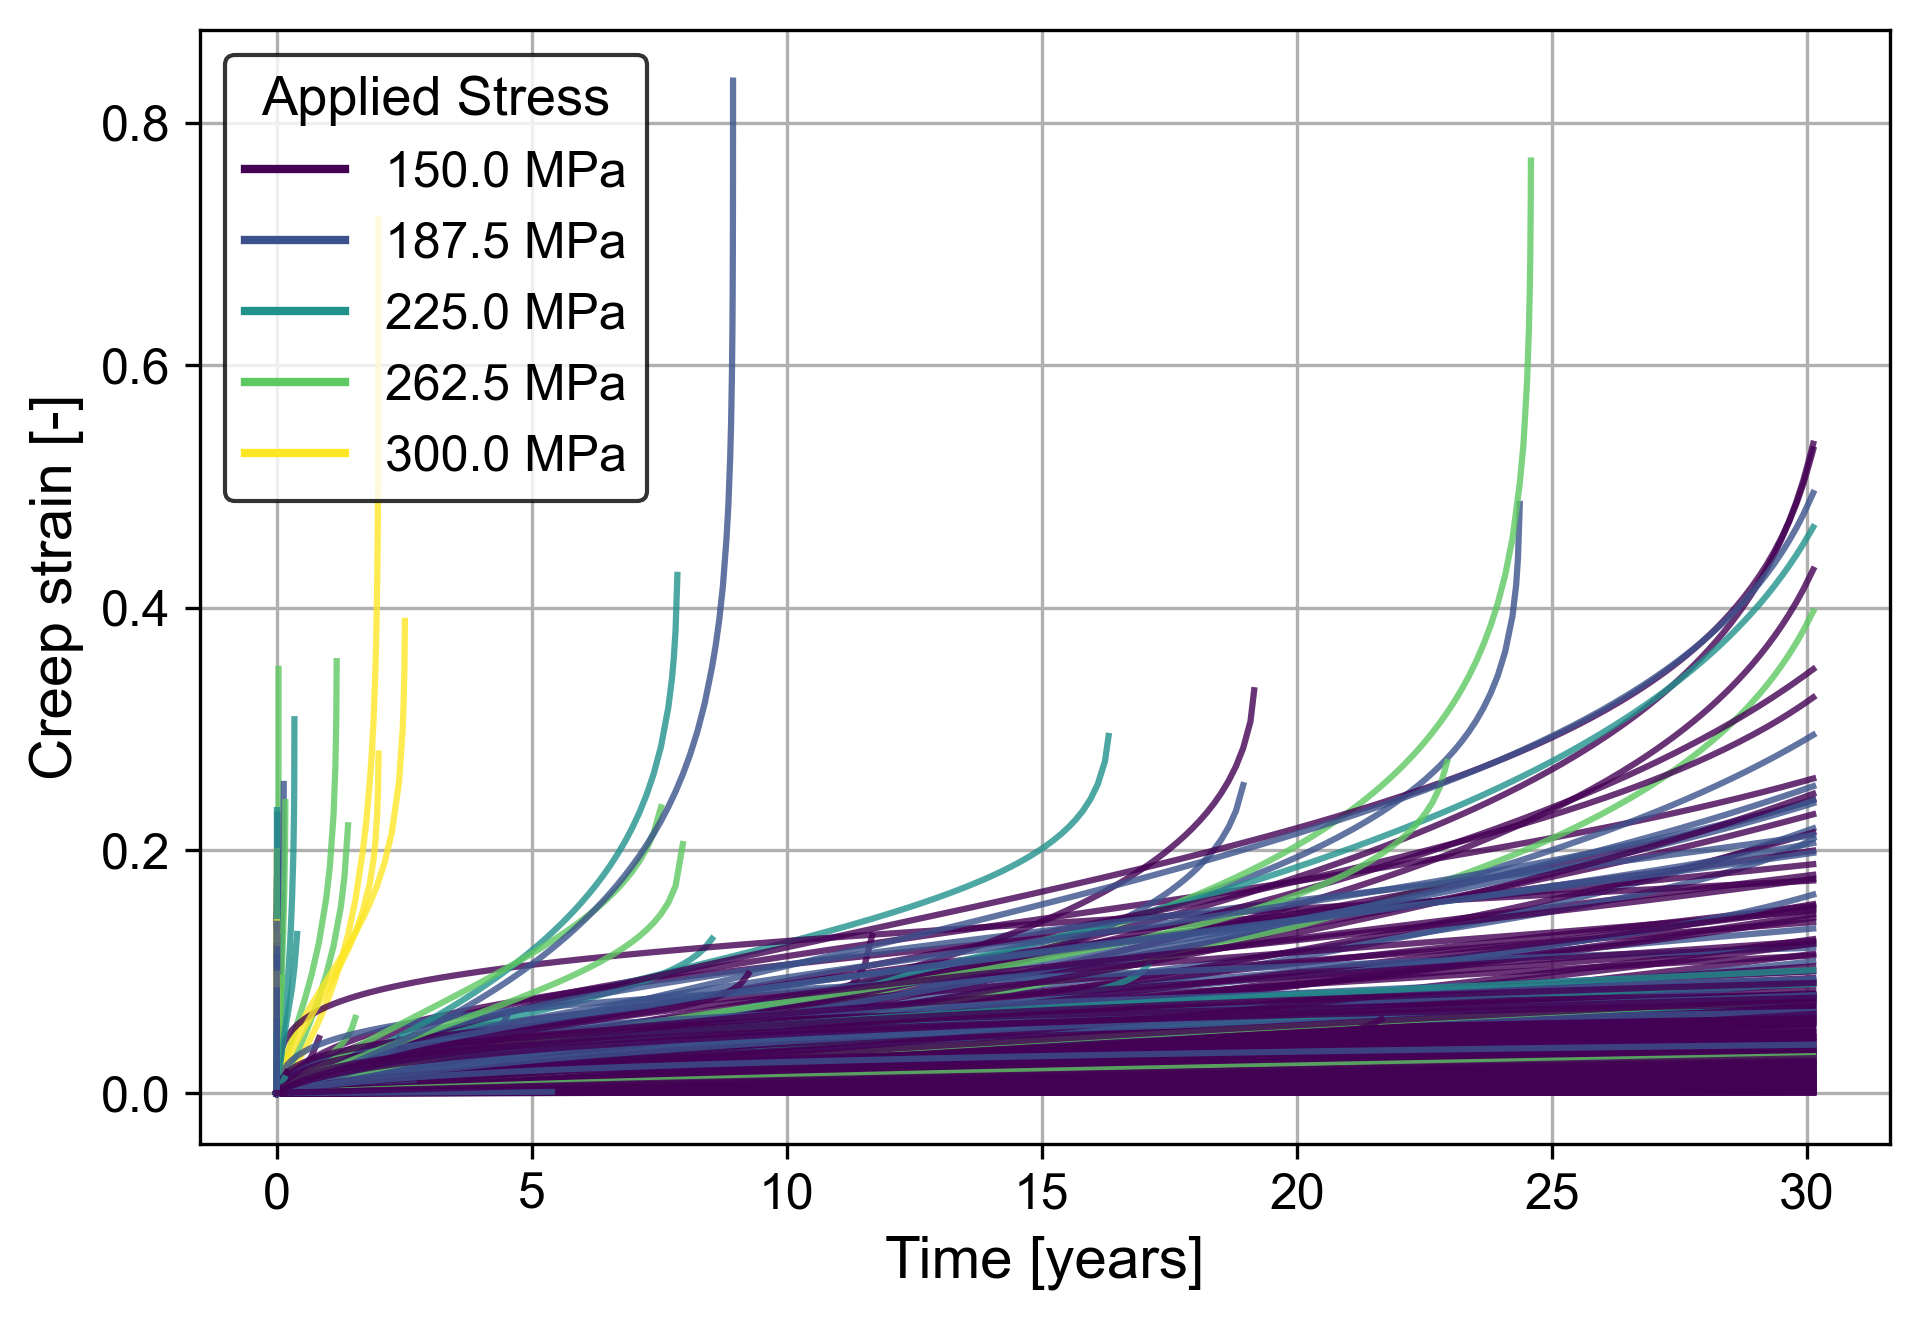
\includegraphics[width=0.9\textwidth]{figures/creep_curves_AL_lagamine.png}
			\captionof{figure}{Creep curves sampled from AL.}
			\label{fig:creep_curves_AL_lagamine}
		\end{center}
	\end{minipage}
	
	\begin{table}[H]
		\centering
		\caption{Summary of Active Learning Results}
		\label{tab:al_summary}
		\begin{tabular}{lc}
			\toprule
			\textbf{Description} & \textbf{Value} \\
			\midrule
			Total queries attempted & 2000 \\
			Converged simulations & 980 \\
			Initial training samples & 100 \\
			Model used in loop & MLP (for $\theta$ projection) \\
			Sampling strategy & Differential Evolution + Feasibility Filter \\
			\bottomrule
		\end{tabular}
	\end{table}
	
	\clearpage
	
	\ifstandalone
		\printglossary
		\printbibliography[heading=bibintoc]
	\fi
	
\end{document}
                                              \clearpage
    \documentclass[class=scrbook, crop=false]{standalone}
\usepackage[subpreambles=true]{standalone}
\ifstandalone
    \input{../settings+/settings}
\fi

% ----------------------------------------------------------------------------
%                               Discussion
% ----------------------------------------------------------------------------
\begin{document}
  
\chapter{Discussion}
\label{Chapter::Discussion}

This chapter presents a critical evaluation of the findings reported in Chapter~\ref{Chapter::Results}. The discussion covers key aspects such as simulation quality, empirical and data-driven creep curve representations, regression model performance, and the effectiveness of active learning. Interpretations are grounded in the context of the modeling goals and limitations inherent to the workflow.

\section{Simulation Quality and Synthetic Data}

The input parameter ranges defined for dataset generation (Table~\ref{tab:param_ranges}) were designed to broadly capture material behavior under varying stress conditions. While 3376 simulations were generated successfully during initial sampling, only 980 of 2000 additional samples converged during the active learning loop. This suggests that certain regions in the parameter space, although mathematically plausible, may lead to numerical instabilities or physically infeasible behaviors when processed by the Lagamine solver.

The discrepancy in convergence rate emphasizes the importance of convergence-aware sampling strategies, particularly in iterative learning frameworks. The use of a feasibility filter in later stages was a step in this direction but may require further refinement to enhance sampling efficiency.

\section{Empirical Model Fits}

Both empirical models, the $\theta$-projection model and the three-parameter exponential model, were evaluated for their ability to represent the simulated creep curves. The $\theta$-projection model achieved superior performance in terms of RMSE and deviation (Figures~\ref{fig:theta_fit_whole_set} and \ref{fig:theta_fit_max_deviation}) from the original creep curves, consistently producing better fits across the dataset.

The three-parameter model, while offering a simplified representation of the creep behavior, showed a slightly higher deviation (Figure~\ref{fig:three_stage_fit_whole_dataset}). This suggests that although both models are capable of capturing the general creep phases, the $\theta$-projection model is more flexible in representing nuanced variations in creep behavior.

The use of empirical models for creep prediction has been explored in earlier studies, though typically in narrower or less integrated settings. For instance, Brown and Korringa~\cite{brown2002extrapolation} established the effectiveness of the $\theta$-projection model in long-term creep extrapolation for power plant steels, showing strong agreement with experimental data. Our findings confirm this flexibility, as the $\theta$-projection model achieved the lowest RMSE across the dataset (see Table~\ref{tab:model_errors}).

In contrast, recent work by Dacol and Caetano~\cite{dacol2022modelling} applied the three-parameter exponential model for unified creep phase modeling. While computationally simple, our results indicate that this model slightly underperformed compared to the $\theta$-model in capturing creep curve shape, especially in the tertiary regimes.

\section{Dimensionality Reduction of Creep Curves}

Principal Component Analysis (PCA) was applied using three different strategies for handling non-uniform input lengths. Zero padding and normalization by rupture time led to high variance capture in fewer components, with the first 2–5 components explaining over 95\% of the total variance (Figures~\ref{fig:pca_variance_zero}, \ref{fig:pca_variance_max}, \ref{fig:pca_variance_norm}). These results suggest that the time-dependent creep behavior can be effectively compressed into low-dimensional representations, especially under standardized input transformations.

Kernel PCA (KPCA), using both RBF and polynomial kernels, showed varying reconstruction quality depending on the kernel parameters and data preprocessing. The polynomial kernel performed better under max strain padding (Figure~\ref{fig:kpca_max_fill}), but the RBF kernel performed slightly better under zero padding and normalization approach (Figures~\ref{fig:kpca_zero_fill}, \ref{fig:kpca_norm_rupture_time}). The reconstruction with normalization by rupture time captured global curve shape better.

Out of the different strategies used for handling the non-uniform input vector lengths, zero padding and the max strain padding tends to capture the artifacts and the actual creep characteristics information gets to be undermined. The normalization approach works better as it doesn't introduce any artifacts during the training stage of the models.

These findings imply that while PCA captures linear variance effectively, KPCA better handles nonlinearity at the cost of interpretability and model complexity. But these data-driven models does not seem to represent the creep curves well when it comes to the teritiary stage of creep.

\section{Supervised Regression of Material Model Parameters}

The inverse modeling task involved predicting seven Morch model parameters from simulated creep curves using four ensemble regression models. Among these, the Voting Regressor achieved the best balance of mean absolute error and $R^2$ score (Table~\ref{tab:model_performance}), indicating robustness across multiple parameter dimensions.

The parity plots (Figures~\ref{fig:RF_regression} to \ref{fig:voting_regression}) doesn't show a good agreement between predicted and true values. Some parameters, particularly those with smaller dynamic ranges, exhibited greater prediction variance, possibly due to reduced signal-to-noise ratios in the training data. The general performance of these models are quite low as is implied in the table~\ref{tab:model_performance}. The reconstructed creep curves (Figure~\ref{fig:curve_recon_model_params}) also does not seem to be well reconstructed.

Overall, ensemble models provided better generalization than individual learners, though performance gains were modest.

\section{Active Learning Efficiency}

The active learning loop aimed to iteratively explore the parameter space for physically meaningful and convergent simulations. The results (Figure~\ref{fig:pairwise_projections}) showed a progressive tightening of the feasible domain, suggesting effective exploitation of the surrogate model. However, only 980 of the 2000 queries resulted in successful simulations, indicating the model's limitations in accurately predicting convergence.

The selection strategy, based on differential evolution combined with a feasibility filter, showed promise but could benefit from integration with uncertainty quantification or probabilistic feasibility modeling to reduce the rate of failed samples. Moreover, while previous studies have used static datasets, our integration of active learning represents a novel hybrid strategy that combines physics-based solvers with intelligent sampling. Although not without convergence challenges, this approach demonstrates potential for data-efficient exploration of high-dimensional material parameter spaces.

\section{Model Performance Comparison}

The final evaluation compared all the creep curve representation methods using RMSE, minimum creep rate error, and time to rupture prediction (Table~\ref{tab:model_errors}). Both empirical models outperformed data-driven methods in terms of RMSE and creep rate error, especially the $\theta$-projection model.

However, time to rupture predictions were not possible using the empirical models, highlighting a tradeoff: empirical models provide accuracy and interpretability, while data-driven models offer generalizability and completeness.

These comparisons underline the importance of choosing representations based on the intended application—whether for interpretability, simulation compatibility, or downstream surrogate modeling.

\section{Limitations of the Approach}
\label{Section::Discussion_Limitations}

While the presented framework demonstrates promising results in creep modeling and surrogate development, several limitations remain that constrain generalizability and reliability:

\begin{itemize}
	\item \textbf{Empirical model dependence:} Both the $\theta$-projection and three-parameter models rely on empirical curve fitting. Although effective for curve compression, they lack physical interpretability with respect to underlying microstructural mechanisms, limiting their value for mechanistic insight.
	
	\item \textbf{Sensitivity to input scaling:} The supervised regression models are sensitive to input scaling and feature ranges. This may affect generalization to unseen loading regimes or materials with different baseline properties.
	
	\item \textbf{Poor inverse model accuracy:} The parity plots and performance metrics (e.g., $R^2 < 0.30$) show that inverse modeling of the full set of Morch material parameters remains inaccurate. This is likely due to parameter non-identifiability, high dimensionality, and limited signal-to-noise ratio in the input data.
	
	\item \textbf{Rupture prediction limitations:} Empirical models, while offering excellent fit, do not natively support time-to-rupture prediction, which limits their applicability for long-term life assessments.
	
	\item \textbf{Active learning convergence challenges:} Although the active learning loop improved sampling efficiency, only 980 out of 2000 queries converged. This indicates that the feasibility filter may not fully capture the solver’s stability domain, leading to wasted queries and computational cost.
	
	\item \textbf{No experimental validation:} The framework is evaluated solely on synthetic FEM-generated data. Without validation against experimental creep data, the true physical accuracy and real-world robustness of the models remain unverified.
	
\end{itemize}

\section{Sensitivity Analysis}
\label{Section::Discussion_Sensitivity}

To better understand the influence of individual input parameters on model outputs, a post hoc sensitivity analysis was performed using the trained surrogate models. This analysis was based on feature importance metrics obtained from tree-based models (e.g., Random Forest and Gradient Boosting), as well as partial dependence plots.

\subsection*{Key Findings}
\begin{itemize}
	\item \textbf{Stress (\(\sigma\)) was the most influential parameter}, consistently showing the highest feature importance across all regressors. This aligns with classical creep theory, where stress is known to exponentially affect creep rate and rupture time.
	
	\item \textbf{Hardening coefficient (\(b\)) showed high non-linear effects}, especially in early creep stages. Its sampling on a logarithmic scale helped capture sharp variations, particularly in primary creep evolution.
	
	\item \textbf{Stress exponent (\(n\)) and creep stiffness (\(K\)) were moderately influential}, primarily affecting the secondary creep rate. However, their individual contributions were often confounded by interaction effects with other parameters.
	
	\item \textbf{Softening parameters (\(S_c, s_c\)) had lower importance}, indicating that tertiary creep behavior was less reliably captured or less variable across the sampled design space.
	
	\item \textbf{Activation energy (\(Q\)) and creep coefficient (\(k_c\)) showed mixed relevance}, depending on the model target. These parameters may require reparameterization or alternative representations for better interpretability.
\end{itemize}

\subsection*{Interpretation}
The analysis reveals that the surrogate models are particularly sensitive to stress and hardening behavior, suggesting that future modeling efforts should focus on these areas for better precision. Additionally, the lower sensitivity to some softening parameters may indicate redundancy or non-identifiability under current data constraints. Incorporating global sensitivity methods such as Sobol or Morris analysis could provide further quantitative insight.




\ifstandalone
	\printglossary
	\printbibliography[heading=bibintoc]
\fi

\end{document}
                                           \clearpage
    \documentclass[class=scrbook, crop=false]{standalone}
\usepackage[subpreambles=true]{standalone}
\ifstandalone
    \input{../settings+/settings}
\fi

% ----------------------------------------------------------------------------
%                               Summary
% ----------------------------------------------------------------------------
\begin{document}

\chapter{Summary and Outlook}
\label{Chapter::Summary_Outlook}

\section{Summary}

This thesis presents a study of applying models for creep curve representations and dataset generation to efficiently model creep behaviour in metallic materials. The approach integrated finite element simulations, empirical curve modelling, dimensionality reduction, supervised learning, and active learning.

Key contributions include:

\begin{itemize}
	\item \textbf{Synthetic Data Generation:} 3376 simulations were performed across a wide parameter space, capturing creep responses under varied loading conditions.
	
	\item \textbf{Empirical modelling:} Creep curves were fitted using the two empirical models. These models showed better accuracy in reconstructing simulation outputs.
	
	\item \textbf{Dimensionality Reduction:} Dimensionality reduction techniques were applied with different padding strategies to solve the problem of having different input vector lengths. Normalization by rupture time enabled effective compression into low-dimensional spaces.
	
	\item \textbf{Regression modelling:} Ensemble regressors predicted material parameters from creep curve features.  This approach did not work due to the ill-posedness of the inverse problem.
	
	\item \textbf{Active Learning:} A feasibility-guided loop using differential evolution added 980 new convergent samples from 2000 queries, enhancing model diversity and coverage.
\end{itemize}

\section{Outlook}

Several opportunities for further work remain:

\begin{itemize}
	\item \textbf{Material and Load Diversity:} Extending the framework to complex loading conditions (e.g., accelerated creep tests, thermal cycling) would enhance applicability.
	
	\item \textbf{Experimental Validation:} Incorporating real creep test data would help benchmark and calibrate the models, improving reliability.
	
	\item \textbf{Uncertainty Quantification:} Future models should include confidence bounds on predictions, e.g., via Gaussian processes or Bayesian ensembles.
	
	\item \textbf{Integration Potential:} The trained models can be embedded in digital twin workflows to enable automation and foster reproducibility of the results by structuring and saving data according to the FAIR data principles.
\end{itemize}

\section{Concluding Remarks}

This thesis presents a first step toward the integration of data-driven modelling with physics-based simulation for the analysis of creep behaviour, particularly in the context of the AID4GREENEST project. The proposed workflow aims to support the correlation of accelerated creep test results with standard long-term indicators, thereby helping industry move toward faster and more cost-effective testing strategies.

Overall, the methodology demonstrates how hybrid approaches can complement existing simulation pipelines and serve as a foundation for future extensions involving real experimental data and varying load conditions.

\end{document}
                                              \clearpage
    \documentclass[class=scrbook, crop=false]{standalone}
\usepackage[subpreambles=true]{standalone}
\ifstandalone
    \input{../settings+/settings}
\fi

% ----------------------------------------------------------------------------
%                               Acknowledgments
% ----------------------------------------------------------------------------
\begin{document}

\chapter{Acknowledgments}
\label{Chapter: Acknowledgments}

I would like to express my sincere gratitude to Prof. Dr. Christoph Eberl for his contributions made as the examiner of this thesis study. I also extend my gratitude to Prof. Dr. Anne Marie Habraken for happily agreeing to be my second examiner and for making significant contributions to this thesis from her ongoing research.
 


\end{document}
                                      \clearpage

    % Bibliography
    \printbibliography[heading=bibintoc]                            \cleardoublepage

    % -------------------------------------------------------------------------------
    % Appendix and Glossary
    % -------------------------------------------------------------------------------
    \pagenumbering{Alph} % A, B, C..

    % Appendix
    \documentclass[class=scrbook, crop=false]{standalone}
\usepackage[subpreambles=true]{standalone}
\ifstandalone
    \input{../settings+/settings}
\fi

% ----------------------------------------------------------------------------
%                                 Appendix
% ----------------------------------------------------------------------------
\begin{document}
\appendix

\chapter{}
\addcontentsline{toc}{chapter}{Appendix A: Full Pairwise Projection Maps}
\label{Appendix::PairwisePlots}

\begin{figure}[H]
	\centering
	\begin{tabular}{cccc}
		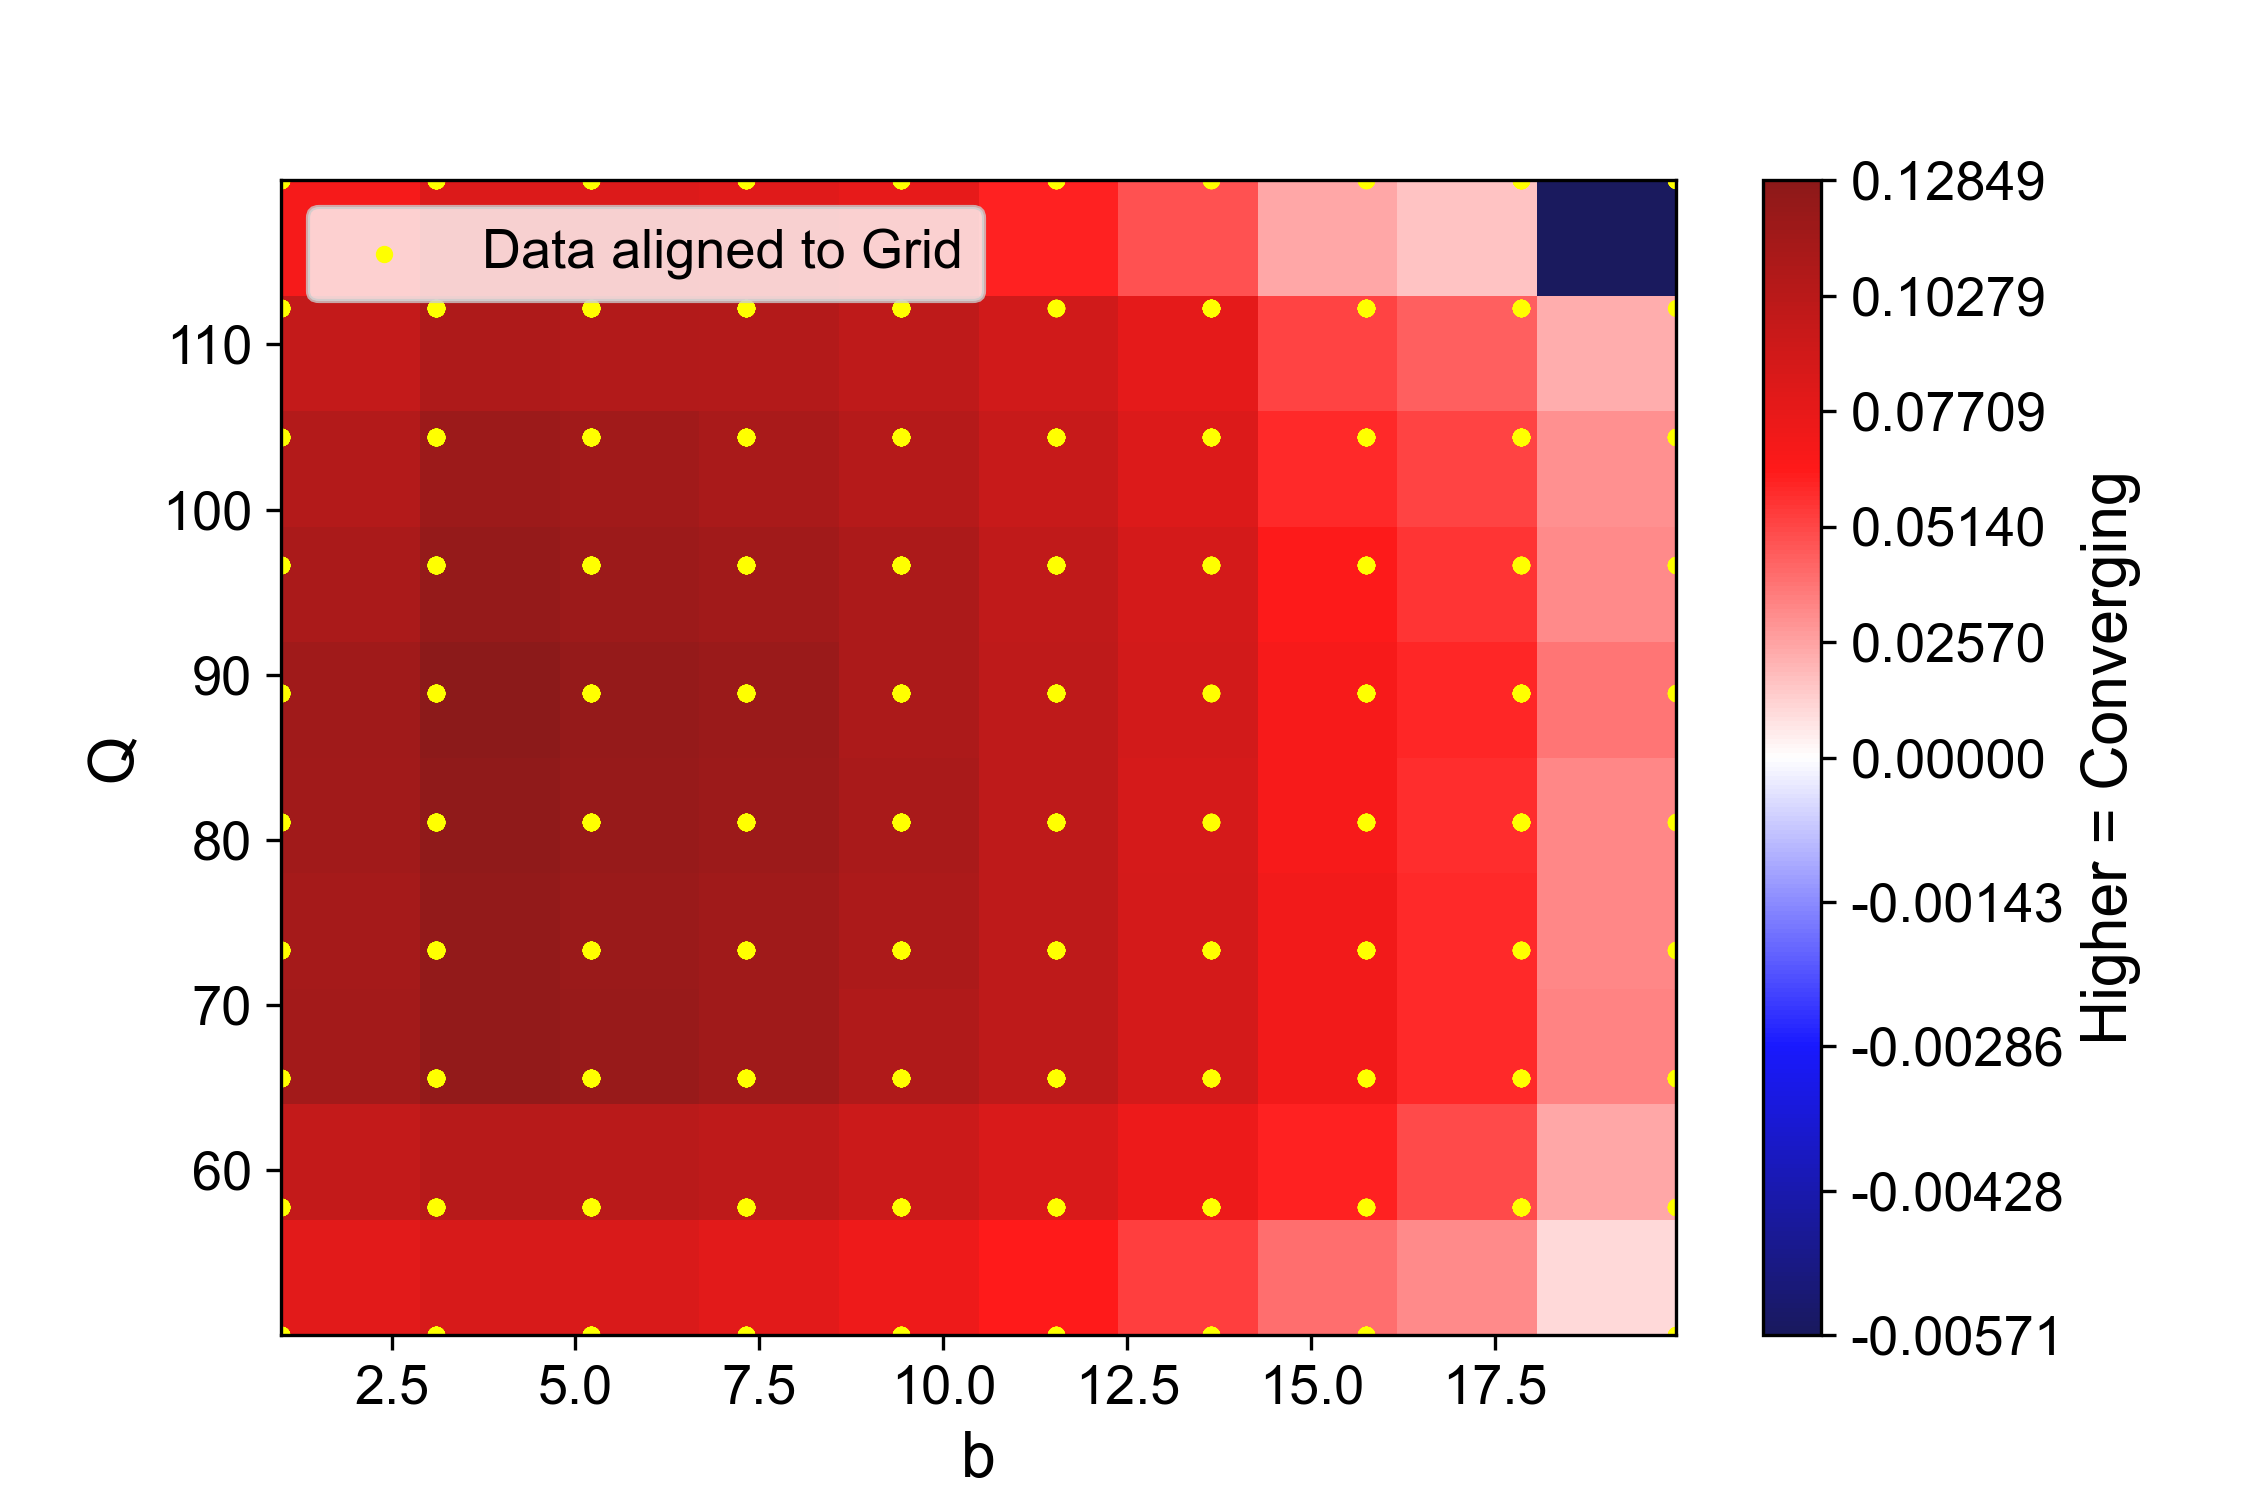
\includegraphics[width=0.32\textwidth]{figures/convergence/pairwise_projections_1.png} &
		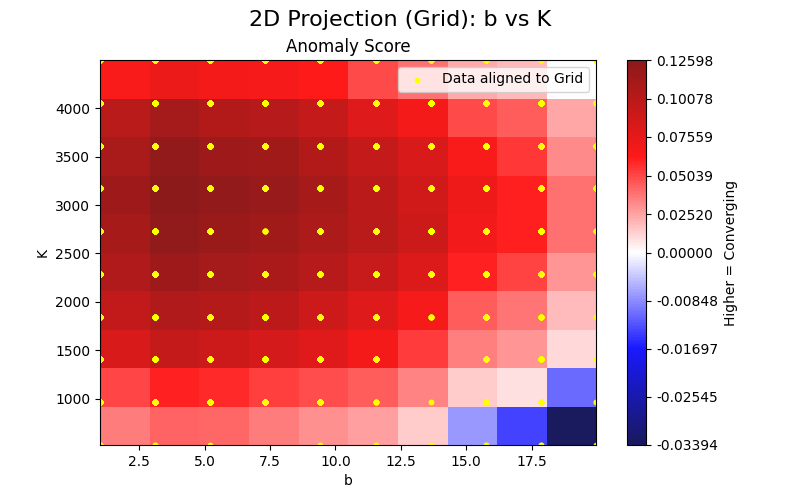
\includegraphics[width=0.32\textwidth]{figures/convergence/pairwise_projections_2.png} &
		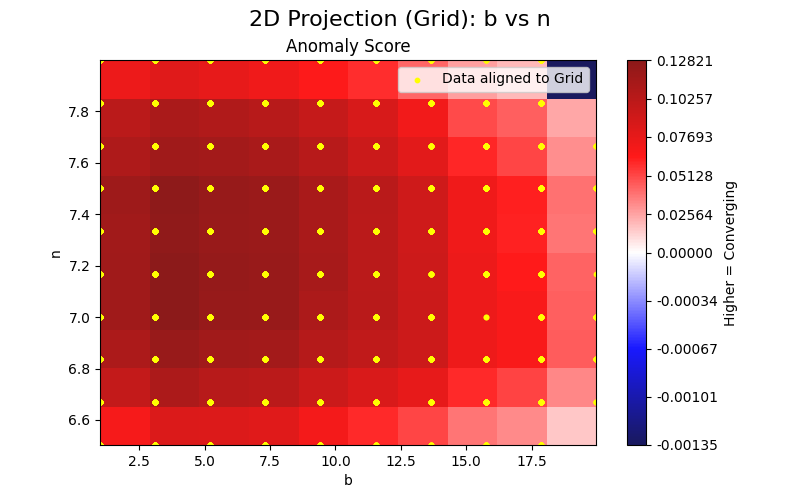
\includegraphics[width=0.32\textwidth]{figures/convergence/pairwise_projections_3.png} \\
		% continue the remaining rows here...
	\end{tabular}
	\caption{Complete set of pairwise scatter plots showing material parameter combinations for the 980 converged simulations in the active learning loop.}
	\label{fig:pairwise_projections_full}
\end{figure}


\section{Section A}
\label{Section::Some Appendix:Section A}

\subsection{Subsection B}
\label{Subsection::Some Appendix:Subsection B}

\Blindtext
\chapter{}
\addcontentsline{toc}{chapter}{Some Appendix2}

\blindtext
\Blindtext

\end{document}
                                             \clearpage

    % print main glossary
    %       type=main           glossary
    %       type=symbolslist    list of symbols
    %       type=acronyms       list of acrononyms
    \printglossary[type=main]

    % Either print all entries or only used entries for all lists
    \glsaddallunused

\end{document}
